%%%%%%%%%%%%%%%%%%%%%%%%%%%%%%%%%%%%%%%%%%%%%%%%%%%
% DOCUMENT CLASS DECLARATION
%%%%%%%%%%%%%%%%%%%%%%%%%%%%%%%%%%%%%%%%%%%%%%%%%%%
%% Use the following options:
% \documentclass[paper type% ("letterpaper" required)
% , one or two sided% ("oneside" or "twoside")%
% , font size% ("12pt" required)%
% , document type% ("these", "memoire", "memoireprojet" or "thesepararticles")%
% , document language ("francais" or "english)%
% , addition options% ("creativecommons" if the document is under the creative commons license, "hyperref", "withAlgo2e" to use algorithm2e package with proper formating)
%]{thETS}

%% Exemple with a Ph.D thesis under creative commons, using hyperref
\documentclass[letterpaper%
, twoside%
, 12pt%
,memoire%
, english%
,creativecommons,hyperref%
]{thETS}

\usepackage[utf8]{inputenc}
\usepackage{graphicx}
\usepackage{amsmath, amsthm, amsfonts, amssymb, amscd, siunitx}
\usepackage{setspace, fancyhdr, float, xfrac, longtable, cite}
\usepackage{wrapfig, lscape, rotating, epstopdf, url}
\usepackage{array, booktabs, listings, latexsym}
\usepackage{tikz, standalone, calc}
\usetikzlibrary{shapes,arrows, decorations.markings}
\usepackage{placeins, multirow}
\usepackage[linesnumbered,plain,vlined]{algorithm2e}
%\usepackage{parskip}
\usepackage{framed, pbox, makecell, caption}
%%%%%%%%%%%%%%%%% For code listings %%%%%%%%%%%%%%%%
\usepackage{listings}
\usepackage{xcolor}
\definecolor{codegreen}{rgb}{0,0.6,0}
\definecolor{codegray}{rgb}{0.5,0.5,0.5}
\definecolor{codepurple}{rgb}{0.58,0,0.82}
\definecolor{backcolour}{rgb}{0.95,0.95,0.92}
\lstdefinestyle{mystyle}{
    backgroundcolor=\color{backcolour},   
    commentstyle=\color{codegreen},
    keywordstyle=\color{magenta},
    numberstyle=\tiny\color{codegray},
    stringstyle=\color{codepurple},
    basicstyle=\ttfamily\footnotesize,
    breakatwhitespace=false,         
    breaklines=true,                 
    captionpos=b,                    
    keepspaces=true,                 
    numbers=left,                    
    numbersep=5pt,                  
    showspaces=false,                
    showstringspaces=false,
    showtabs=false,                  
    tabsize=2
}
\lstset{style=mystyle}
%====================New Thm Declarations====================
% \newcommand{\eop}{\hfill $\sqcap\!\!\!\!\sqcup$} % end of proof
\newtheoremstyle{newThmStyle}% <name>
{3pt}% <Space above>
{3pt}% <Space below>
{}% <Body font>
{}% <Indent amount>
{\itshape \bf}% <Theorem head font>
{:}% <Punctuation after theorem head>
{.5em}% <Space after theorem headi>
{}% <Theorem head spec (can be left empty, meaning `normal')>
%%%%
\theoremstyle{newThmStyle}
\newtheorem{assumption}{Assumption}
\newtheorem{lemma}{Lemma}
\newtheorem{theorem}{Theorem}
\newtheorem{proposition}{Proposition}
\newtheorem{definitionNewStyle}{Definition}

% =========================== For Algorithm =======================================
\let\oldnl\nl% Store \nl in \oldnl
\newcommand{\nonl}{\renewcommand{\nl}{\let\nl\oldnl}}% Remove line number for one line
% New command to remove a certain section from the Table of Contents. 
% Add "\tocless" before "\section{•}" to take it out from the Table of Contents.
\newcommand{\nocontentsline}[3]{}
\newcommand{\tocless}[2]{\bgroup\let\addcontentsline=\nocontentsline#1{#2}\egroup}

%%%%%%%%%%%%%%%%%%%%%%%%%%%%%%%%%%%%%%%%%%%%%%%%%%%
% IMPORTANT: PRINTING WITH THE PROPER MARGINS
%%%%%%%%%%%%%%%%%%%%%%%%%%%%%%%%%%%%%%%%%%%%%%%%%%%
%% If you create a pdf with pdftex, and print it using acrobat reader, set the
%% "scaling" option to "none" to print with the proper margins.
%%%%%%%%%%%%%%%%%%%%%%%%%%%%%%%%%%%%%%%%%%%%%%%%%%%


%%%%%%%%%%%%%%%%%%%%%%%%%%%%%%%%%%%%%%%%%%%%%%%%%%%
% DECLARATION OF AN ADDITION LIST OF REFERENCES
%%%%%%%%%%%%%%%%%%%%%%%%%%%%%%%%%%%%%%%%%%%%%%%%%%%
%% Exemple of an additional list of references called "refs"
% "refs" is used as a suffix to all bibliography related commands
\newcites{refs}{LIST OF REFERENCES}

%%%%%%%%%%%%%%%%%%%%%%%%%%%%%%%%%%%%%%%%%%%%%%%%%%%
% TITLE PAGE OPTIONS
%%%%%%%%%%%%%%%%%%%%%%%%%%%%%%%%%%%%%%%%%%%%%%%%%%%

\title{Development of Output Signal Differentiator for Nonlinear Observer based Trajectory Tracking of a Quadcopter}

\author{Mohammed Basharnavaz KHAN}
\authorcopyright{Mohammed Basharnavaz Khan}

\datesoutenance{April 15, 2020}

\datedepot{April 20, 2020}

\directeur{Mr. }{Maarouf Saad}{Departement of Electrical Engineering, École de technologie supérieure}

\president{Mr. }{Guy Gauthier}{Departement of Electrical Engineering, École de technologie supérieure}

\jury{Mr. }{Jean-Pierre Kenné}{Departement of Mechanical Engineering, École de technologie supérieure}

\juryB{Mrs. }{Hannah Michalska}{Department of Electrical and Computer Engineering, McGill University}

%%%%%%%%%%%%%%%%%%%%%%%%%%%%%%%%%%%%%%%%%%%%%%%%%%%
% CHANGING THE NAME OF THE DIPLOMA
%%%%%%%%%%%%%%%%%%%%%%%%%%%%%%%%%%%%%%%%%%%%%%%%%%%
%% It is possible to change the name of the diploma by redefining
% the command \lediplome, as follows:
%\renewcommand{\lediplome}{OF A MASTER’S DEGREE\\WITH THESIS IN ELECTRICAL ENGINEERING\\M.A.Sc.}

\listfiles

%%%%%%%%%%%%%%%%%%%%%%%%%%%%%%%%%%%%%%%%%%%%%%%%%%%
% ACTUAL DOCUMENT
%%%%%%%%%%%%%%%%%%%%%%%%%%%%%%%%%%%%%%%%%%%%%%%%%%%
\begin{document}

\pagenumbering{Roman}
%%- Title page -%%
\maketitle
%%- Jury presentation -%%
\presentjury
%%- Foreword -%%
%\begin{foreword}
%\lipsum[1] 
%\end{foreword}


%%- Acknowledgements -%%
\begin{acknowledgements}
I want to express my gratitude to several people who have helped me constantly throughout my academic endeavour to produce this thesis.

I would like to thank Professor Hannah Michalska who patiently helped me develop my mathematical understanding to engage in the development of kernel methods of estimation in RKHS. I learnt a great deal on conducting research under constraints of time and resources.

I would also like to thank Professor Maarouf Saad without whom this thesis would not be possible. He has been instrumental in the developments which made it possible to implement the methods on a practical application. Working under his supervision has taught me a great deal on the effective ways of executing a practical research project.

I convey my gratefulness to my peers namely Nuradeen, who guided me though the implementation of algorithms on the quadcopter and Shaunak, Debarshi and Abhishek who helped me understand their work on which the KDO is based. 

Lastly I would like to thank Claire. 
\end{acknowledgements}

%%- Summary -%%
\begin{summary}{Dévelopement d'un différentiateur de signal de sortie pour un observateur non linéaire pour la poursuite de trajectoire d’un quadricoptère }{Quadrotor UAV; Backstepping control; Sliding mode control(SMC); Nonlinear disturbance observer(NDO); Super-twisting Observer(STO); Kernal Differential Observer(KDO)}
Une approche non asymptotique pour l'estimation de l'état complet pour la construction d'un observateur de perturbations externes non linéaire est présentée dans ce mémoire. L'observateur développé est nommé Kernel Differential Observer (KDO). Il est envisagé que le KDO fonctionnerait en conjugaison avec des algorithmes de contrôle pour obtenir un suivi robuste d'un quadrirotor sous des perturbations externes. Le quadrirotor est un système sous-actionné non linéaire à entrées multiples et sorties multiples avec un haut degré de couplage dynamique. Le contrôleur de suivi basé sur l'observateur vise à suivre une trajectoire de sortie de référence donnée en termes de position et de lacet du quadrirotor.

Le KDO utilise une structure locale de modèle LTI de quatrième ordre sur la sortie de position et d'attitude du quadrirotor, dans une fenêtre mobile de longueur fixe qui avance à mesure que le temps avance. La structure du modèle s'adapte également au fil du temps pour s'adapter au mieux à la mesure de la position et de l'attitude tout en dérivant simultanément la position et l'attitude pour obtenir les vitesses et accélérations respectives, estimant ainsi l'état complet du quadrirotor. Pour ce faire, l'observateur, à chaque itération, estime les paramètres du noyau qui décriraient le mieux la dynamique sous-jacente des quadrirotors non linéaires. Il existe quelques approches présentées pour estimer les paramètres, l'algorithme de régression dynamique par crête (ridge) ou la méthode des moindres carrés d'erreur de sortie résiduelle de la reproduction de l'expression du noyau (Kernel). L'algorithme de régression par crête dynamique est coûteux en calcul car il utilise l'optimisation par recherche itérative, tandis que la méthode des moindres carrés donne une solution exacte au problème d'optimisation. Le choix de la méthode dépend des ressources de calcul et des contraintes de temps de l'application.

Une fois que l'état complet du quadrirotor est disponible, le KDO estime les perturbations externes afin de poursuivre le suivi. Pour évaluer l'efficacité du suivi, l'observateur et le contrôleur sont testés en simulation et en temps réel sur un quadrirotor PIXHAWK S500. La simulation et les résultats en temps réel confirment que la méthodologie adaptative et l'estimation de l'état complet par différenciation du signal de la sortie présentée ici sont supérieures aux méthodes asymptotiques trouvées dans la litérature.

\end{summary}

%%- Abstract -%%
\begin{abstract}{Quadrotor UAV; Backstepping control; Sliding mode control(SMC); Nonlinear
disturbance observer(NDO); Super-twisting Observer(STO); Kernal Differential Observer(KDO)}
A non-asymptotic approach for full state estimation for the construction of a nonlinear external disturbance observer is presented in this thesis. The developed observer is named, Kernel Differential Observer (KDO). It is envisioned that the KDO would work in conjugation with control algorithms to achieve robust tracking of a quadcopter under external disturbances. The quadcopter is a nonlinear multiple-input multiple-output underactuated system with a high degree of coupling between its component states. The observer-based tracking controller aims to track a given reference output trajectory in terms of the position and the yaw of the quadcopter.

The KDO employs a local fourth-order LTI model structure on the position and attitude output of the quadcopter, within a fixed-length sliding window which moves ahead as time progresses. The model structure also adapts over time to best fit the measurement of the position and attitude while simultaneously also differentiating the position and attitude to obtain the respective velocities and accelerations, thereby estimating the full state of the quadcopter. In order to do this, the observer, in each iteration, estimates the parameters of the kernel that would best describe the underlying nonlinear quadcopter dynamics. There are a couple of approaches presented to estimate the parameters, dynamic ridge regression algorithm or least square method of residual output error from reproducing kernel expression. The dynamic ridge regression algorithm is computationally expensive as it employs optimization by iterative search, while the least square method gives an exact solution to the optimization problem. The choice of method depends on the computational resources and time constraints of the application.

Once the full state of the quadcopter is available the KDO estimates the external disturbances in order to achieve continued tracking. To evaluate the effectiveness of tracking the observer and controller are tested out in simulation and in real-time on a PIXHAWK S500 quadcopter. The simulation and real-time results confirm that the adaptive methodology and full state estimation by signal differentiation of the output presented here are superior to the asymptotic methods found in the literature.


\end{abstract}

%%- Table of contents -%%
\tableofcontents

%%- List of tables -%%
\listoftables

%%- List of figures -%%
\listoffigures

%%- List of abbreviations -%%
\begin{listofabbr}[3cm]
\item[MAV]    Micro Aerial Vehicle
\item[UAV]    Unmanned Aerial Vehicle
\item[NDO]    Non-Linear Disturbance Observer
\item[STO]    Super Twisting Observer
\item[KDO]    Kernel Differential Observer
\item[KDS]    Kernel Double Sided
\item[RKHS]   Reproducing Kernel Hilbert Space
\item[SISO]   Single Input Single Output
\item[MIMO]   Multiple Input Multiple Output
\item[LTI]    Linear Time Invariant
\item[PID]    Proportional Integral Derivative 
\item[LQR]    Linear Quadratic Regulator
\item[SMC]    Sliding Mode Controller
\item[ROS]    Robot Operating System
\item[PWM]    Pulse Width Modulation

\end{listofabbr}


%%- List of symbols -%%
\begin{listofsymbols}[3cm]
\item [$p$] Position vector of quadcopter
\item [$\Theta$] Attitude vector of quadcopter
\item [$\mathcal{B}$] Body Frame of the quadcopter
\item [$\mathcal{I}$] Earth frame
\item [$\phi$] Roll angle
\item [$\theta$] Pitch Angle
\item [$\psi$] Yaw angle
\item [$s(.)$] sine function
\item [$c(.)$] cosine function
\item [$F_{prop}$] Force vector acting on the quadcopter in body frame
\item [$T_{prop}$] Thrust vector acting on the quadcopter in body frame
\item [$m$] Mass of quadcopter
\item [$I_i$] Moment of inertia along an axis
\item [$r_i$] Ratio of inertia parameter of the quadcopter
\item [$q_i$] Ratio of inertia parameter of the quadcopter
\item [$U_i$] Control input to the quadcopter
\item [$d_i$] Disturbance to a quadcopter subsystem
\item [$\hat{d_i}$] Estimated disturbance by an observer 
\item [$t_k$] Time instant of estimation using KDO
\item [$\zeta$] General flat output variable
\item [$\mathbf{w_{\zeta_k}}$] Kernel parameters for the $\zeta$ estimation at the $i$th window
\end{listofsymbols}


\cleardoublepage
\pagenumbering{arabic}
% Marginpar to the left of the document
\reversemarginpar
%%%%%%%%%%%%%%%%%%%%%%%%%%%%%%%%%%%%%%%%%%%%%%%%%%%
% THESIS 
%%%%%%%%%%%%%%%%%%%%%%%%%%%%%%%%%%%%%%%%%%%%%%%%%%%

\begin{introduction} \label{Chap:Intro}
Engineers are often interested in controlling the behaviour of their surroundings or a part of it, often referred to as a "system" in order to provide desirable results in domains such as transportation, manufacturing etc. In order to do so, engineers develop control systems which are interconnected components forming a system configuration that will provide a desired system response  \citep{bishop1996modern}. These components are usually actuators, micro-controllers and power electronics that drive the actuators and software, which contains the logic or algorithms which determine the actuation signals.

As time progressed, the systems have become increasingly complicated, with multiple interrelated variables that are needed to exhibit the behaviour. To control these systems,  maybe more than one actuator used in an attempt to make the system or plant have the desired behaviour. These types of control, such systems are called Multiple-input control systems. Most advanced control systems use the output of the plant or the system to be controlled as an essential criterion to compute the subsequent control signals to the system. These types of control systems are called Closed Loop Control systems. Usually, there is an error in the measurement of the plant output, known as measurement noise, which is attempted to minimize by using filtering algorithms that aid the control systems by providing more accurate information compute the intended control signal. In some cases, control systems employ the use of observers, which estimate the state of the system or external disturbances that affect it. This thesis aims at developing an observer based on an algebraic estimator to observe external aerodynamic disturbances and compare it with a couple of other observers in the literature. 

\tocless \section{Literature Review}
For a long time now, quadcopters have been of interest to control engineers as they present interesting challenges in several domains of control theory. It is a Multiple Input Multiple Output system with six degrees of freedom and twelve components that describe its complete state. Since it is an unmanned aerial vehicle with just four inputs in the form of rotor speeds to the four individual rotors (that act as actuators to this system), it is also classified as an under-actuated system \citep{wang2016dynamics}. These complexities have led to substantial research in different control strategies for quadcopters. 

\tocless \subsection{Quadcopter Modeling and Control}
The mechanical construction of a quadcopter is quite simple and inexpensive. It consists of placing two sets of rotating propellers on opposite ends of beams placed rigidly at right angles to each other. The mechanical system is considered as a rigid body in 3-dimensional space with six degrees of freedom, three rotational and three translational. The orientation of the quadcopter is usually expressed as a set of Euler angles or quaternions. Euler angle representation poses the problem of gimble lock \citep{RN85}, \citep{RN84}. The gimble lock phenomenon presents singularities where one degree of freedom is lost, resulting in singularities, which restricts trajectory tracking capabilities of the quadcopter. 
The dynamics of the quadcopter has been described in detail in multiple sources in literature, \citep{RN86}, \citep{RN87} and \citep{RN88}. Considering the dynamical model as two subsystems, angular and positional subsystem, it can be seen that the angular kinematics is independent of the linear motions, although the linear kinematics are dependent on the orientation of the quadcopter, \citep{RN89}. Therefore most souces of literature consider the quadcopter to have two subsystems, position and attitude subsystems and a control loop to control these individual subsystems. The outer loop controls the position \citep{RN90}, \citep{RN91} and the inner loop controls the attitude \citep{RN92}, \citep{RN93}. Most of the times, having accurate dynamic models is not enough to have robust control of a quadcopter as the dynamics are affected by factors such as model uncertainties, measurement inaccuracies and external disturbances. Model uncertainties arise due to model linearizations, inaccurate system parameters and assumptions in motor dynamics. One way of addressing model inaccuracies is through experimental identification of system parameters such as moments of inertia, mass, motor dynamics etc., suggested through  \citep{RN94}, \citep{RN95}, \citep{alexis2011model}. Another approach towards model uncertainties is to consider them as external disturbances and try to mitigate them with appropriate observer-controller strategies. External disturbances can be in the form of wind gusts \citep{RN97}, unstable payloads \citep{RN98}, actuator failure or irregular battery voltages.


There has been extensive research conducted in various control methods for quadcopters. Linear controllers are efficient in maintaining the quadcopter in the hovering position due to linearization around the setpoint (desired hover position). The classical approaches of proportional-integral-derivative (PID) control and linear quadratic regulator and their combination were presented in \citep{RN99}. \citep{RN100} uses the backstepping controller with an Extended Kalman Filter (EKF) to control a quadcopter for indoor flights. \citep{RN102} uses sliding mode control for robust tracking control of a quadcopter subjected to wind disturbances. \citep{RN103} uses both backstepping and SMC to control the rotation and the position subsystems of the quadcopter and concludes that the backstepping controller provides controllability of the orientation angles under relatively high perturbations. Model predictive control methods \citep{RN104}, \citep{RN105}, \citep{RN106} are suitable for control of multivariate systems, such as quadcopters, that are governed by constrained dynamics as compared to the classical methods such as the PID or LQR mentioned earlier.


To improve the controllability under external disturbances, robust controllers such as the nonlinear H$_\infty$ control algorithm \citep{RN108} are used for path tracking where the MPC controller tracks the path and the H$\infty$ stabilizes the rotational subsystem. This method is susceptible to additional disturbances through the linearization of the nonlinear dynamics. \citep{RN109} proposes a similar solution but is still susceptible to additional disturbances. To overcome this problem, observer-based control algorithms  have been proposed in \citep{RN110}, \citep{RN111}, \citep{RN112}, \citep{RN113}. Recent advancements in this approach have been done by \citep{RN114}, \citep{RN116}, \citep{RN117}. \citep{RN114} proposes backstepping and sliding mode controller in conjugation with the nonlinear disturbance observer (NDO) for trajectory tracking. The NDO is an asymptotic observer which requires an initial estimate to initialize the observer. \citep{RN117} proposes an alternate observer, super-twisting observer (STO), with a faster convergence rate than the NDO, but again requires an initial estimate to initialize the state of the observer. Both \citep{RN114} and \citep{RN117} conduct simulations with smooth sinusoidal external disturbances with information about the initial conditions known to the observers. 
Algebraic estimators provide an estimate of systems without requiring the need for initializers. The literature on this will be discussed later in this section.\\ 
\tocless \subsection{Differentially Flat Systems} \label{subsec:diffflatnessquad}
Differential flatness was introduced in a series of papers by Fliess in the context of differential algebra and Lie-Backland transformations \citep{RN78}, \citep{RN79}, \citep{RN80}. It is a structural property of a system that allows an engineer to parameterize every system variable in terms of set "free" variables of the system \citep{RN77}. 
The differential flatness property of a system provides the possibility of differentially parameterizing system variables in terms of "free variables." In other words, the system variables are functions of the "free variables" and a finite number of derivatives of some or all of them.
Differentially flat systems are systems where the full state of the system and the input to the system can be determined from a set of outputs, which is equal to the number elements in the set of inputs to the system \citep{RN73}. 
\citep{RN81} mentions the quadcopter system to be a differentially flat system.  The relations between thrust, $T$ and torques along  $x$, $y$ and $z$ axes are given as functions of the states of the system but omits the derivation of these relationships. \citep{mellinger2011minimum} can be considered to be the first paper that proves the differential flatness of the quadcopter system without considering the rotor drag. \citep{faessler2017differential} extends upon this work but points out a couple of incorrectness found out in \citep{mellinger2011minimum}. It provides the correct approach to prove the differential flatness property, while also assuming rotor drag in the derivation. It is recommended that for the exhaustive proof, one refer to the corrected and extended version in \citep{faessler2017differential}. Having established the property of flatness of a quadcopter system allows us to implement algebraic estimation techniques on the output of the quadcopter. 

\tocless \subsection{Algebraic Differentiation and the Double Sided Kernel}
The Double-Sided Kernel method was developed for state estimation of differentially flat second order systems in \citep{RN76}. The double-sided kernel does not exhibit any singularities, as did the previous algebraic estimators in \citep{RN75}. The method expresses the system states as a function of output and/or its time derivatives using the properties of differentially flat systems. The method simultaneously computes the parameters and uses them to find higher derivatives of the system.


Although the algebraic estimators prove to be superior to their asymptotic counterparts, they have not yet been implemented on a real-time application that is subjected to several constraints of time, computational power and available memory. 

\tocless \section{In This Thesis}
Autonomous control systems rely on observers to estimate external disturbances in the system being controlled. Signal differentiation plays a crucial role in the construction of nonlinear disturbance observers. In the light of the introduction of algebraic estimation of SISO differentially flat systems, the general objective of this thesis is to develop an algebraic observer for the purpose of constructing nonlinear controllers for dynamical systems. Specifically, the nonlinear disturbance observers (Non-linear Disturbance Observer, Supertwisting Observer and Kernel Differential Observer) will be employed to estimate aerodynamic forces during quadcopter flights, in simulation and practice.

The kernel-based algebraic differentiators will employ a fourth-order LTI structure over a moving window in conjunction with dynamic ridge regression. 
The performance of three different observers will be compared in closed-loop with a tracking control of a quadcopter. The other observers in the study are:
\begin{itemize}
\item The nonlinear disturbance observer presented in \citep{RN114} 
\item The super-twisting sliding mode observer \citep{RN117}
\end{itemize}
As mentioned above, based on the literature survey and preliminary simulations, the bottleneck in implementing algebraic estimators in practical systems is the computational effort, which several microcontrollers are not able to provide.
The following steps are made towards achieving the general objective of this project: 

\begin{itemize}
\item Develop signal differentiators based on algebraic differentiation. Extend methods presented in \citep{RN83} to a MIMO system and apply full state observation on a quadcopter. Develop an observer to estimate external disturbances using full state estimation of the quadcopter while using only the translational angles and positional coordinates. 
\item Investigate the stochastic properties of the double-sided kernel when the output measurements have white noise. Explore the computational aspects of the double-sided kernel to implement the Kernel Differential Observer in real-time.
\item Test the effectiveness of the developed KDO against observers found in the literature in simulation using chaotic and other types of disturbances while the asymptotic observer has no information on the initial state of the system. 
\item Develop a distributed computing framework in Robot Operating System (ROS) to implement the KDO in real-time on the quadcopter and compare it against existing observers.
\end{itemize}

The thesis will focus on the development of kernel-based algebraic differentiators of signals for estimation of disturbances from observation of the system inputs and outputs. A comparison of existing methods for
disturbance estimation will be carried out by way of simulations.
The project will focus on the development and implementation of algebraic observers on quadcopters with limited processing abilities. To achieve the above objectives the following tools will be used:
\begin{itemize} [label={}]
\item {\bf MATLAB/Simulink:} Primarily intended for simulations. The quadcopter models will be developed in Simulink, while Simulink offers multiple solvers depending on the specific constraints of the problem
\item {\bf ROS, PX4:} This would be the practical framework on which estimation algorithms would be evaluated
\item {\bf C++:} Implementation of algorithms will be done as ROS nodes coded in C++ \\Editors for the above languages are: Eclipse, Atom
\end{itemize}


	 
\tocless \section{Thesis Organization}
\begin{itemize} [label={}]
\item {\bf Introduction:} This chapter introduces control systems while giving a brief background into the different types of techniques in control available in the literature. It presents the literature reviewed on quadcopter modelling and control, while also presenting the concept of differential flatness. The supporting literature on algebraic differentiation is presented, which is used to develop the Kernel Disturbance Observer. 
\item {\bf Chapter \ref{Chap:Quad}:} This chapter focuses entirely on presenting the dynamical model of the quadcopter and its differential flatness property. Mathematical definitions of differential flatness is provided along with an example to illustrate this property. The chapter concludes by presenting the simulation and practical methods used at GREPCI Robotics Lab to identify the parameters of the quadcopter.
\item {\bf Chapter \ref{Chap:Observers}:} This chapter presents the two observers, Nonlinear Disturbance Observer and Super-Twisting Observer, from the literature that will be compared against the Kernel Disturbance Observer. The chapter also presents the observer based control tracking scheme that is used. 
\item {\bf Chapter \ref{Chap:KDO}:} This chapter presents the Kernel Disturbance Observer that is developed in this thesis. The KDO is developed using the algebraic differentiators presented previously in the Introduction chapter. Section \ref{Sec:ThmKdo} develops closed-form expressions for parameter estimation using repeated integration and kernel reproducing property. The chapter concludes by presenting an example of using Kernel Estimation techniques on a non-linear system with white Gaussian noise. 
\item {\bf Chapter \ref{Chap:ResultsSim}:} This chapter presents the results of simulation of the observer based controller on the quadcopter. The simulations are conducted in SIMULINK and the disturbances are chaotic unlike the sinusoidal disturbances used in the simulations in literature. 

\item {\bf Chapter \ref{Chap:ResultsPrac}:} The algorithms are validated on an the Pixhawk S500 experimental setup. The chapter details the different components in setting up the distributed computing setup using ROS. The external disturbances are generated using a CONAIR 1600 air blower. The chapter concludes by presenting the root mean square error in tracking in both cases. 

\item {\bf Conclusion:} This chapter provides a conclusion of the work presented in the previous chapters, reiterates the results and suggests future work.
\end{itemize}


\end{introduction}

%%- First demo chapter -%% 
\chapter{Quadcopter Model} \label{Chap:Quad}
The flight principles of a quadcopter have been described in \citep{RN71} and many other works.
A quadcopter has four rotors positioned on its arms of equal lengths. The motors are numbered as No. 1 to No. 4, with opposite motors rotating in the same direction, i.e. No. 1 and No.3 rotate counter-clockwise direction, and No. 2 and No.4 rotate in a clockwise direction. The rotation of the motors provides the upward thrust against the gravity to keep the quadcopter in air. Rotation around an axis is obtained by the rotational speed difference between the motors that are placed perpendicular to it. For instance, rotation around the X-axis is caused by the moment around the X-axis generated by the difference of rotational speed between motors No. 2 and No. 4. which are placed perpendicular to the X-axis. A similar action causes rotation around the Y-axis. The rotation of the rotors exerts a torque on the quadcopter frame due to setting the airflow in rotation. The opposing direction of rotation of the motors maintain yaw stability, and a difference in rotation of motor causes yaw or rotation around the Z-axis.

\begin{figure}[H]
	\centering
	\resizebox{0.75\textwidth}{!}{\fbox{\documentclass{standalone}

\usepackage{tikz}
\usetikzlibrary{shapes,arrows, decorations.markings}

\begin{document}
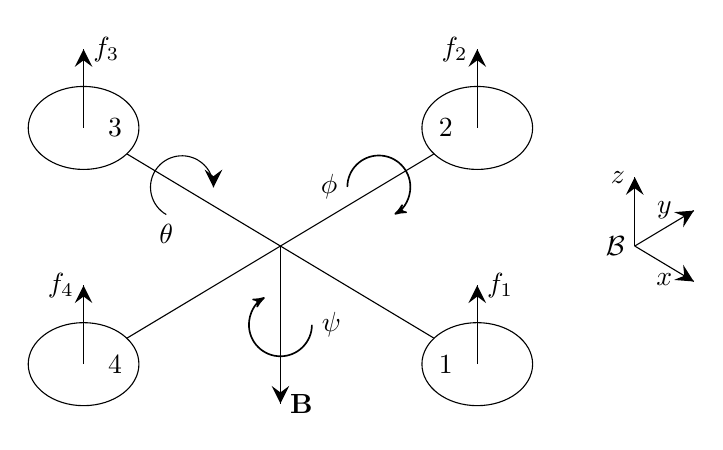
\begin{tikzpicture}
	\tikzstyle{prop} = [draw, ellipse, align=center, minimum width=4em, minimum height=3em]
	\tikzstyle{big_arrow} = [decoration={markings,mark=at position 1 with {\arrow[scale=2,>=stealth]{>}}},postaction={decorate}]
	% Prop nodes
	\node[prop, align=right] (1) at (0,0) {};
	\node[prop, align=left] (2) at (5,0) {};
	\node[prop, align=left] (3) at (5,3) {};
	\node[prop, align=right] (4) at (0,3) {};
	% Label props
	\node[draw=white, rectangle] at (4.6,0) {1};
	\node[draw=white, rectangle] at (4.6,3) {2};
	\node[draw=white, rectangle] at (0.4,3) {3};
	\node[draw=white, rectangle] at (0.4,0) {4};
	
	% Draw 
	% Connect props
	\draw [-] (1) -- node [midway, above] {} (3);
	\draw [-] (2) -- node [midway, above] {} (4);
		
	%Body Weight arrow 
	\draw [big_arrow] (2.5,1.5) -- node [at end, right] {\textbf{B}} (2.5,-0.5);
	% Prop thrust arrows
	\draw [big_arrow] (5,0) -- node [at end, right] {$f_1$}(5,1);
	\draw [big_arrow] (5,3) -- node [at end, left] {$f_2$} (5,4);
	\draw [big_arrow] (0,3) -- node [at end, right] {$f_3$}(0,4);
	\draw [big_arrow] (0,0) -- node [at end, left] {$f_4$} (0,1);
	
	% Draw arcs	
	\draw[big_arrow] (1.05,1.9) arc[radius=0.4, start angle=240, end angle=0] node[at start, below]{$\theta$};
	\draw[->,>=stealth',semithick] (3.35,2.25) arc[radius=0.4, start angle=180, end angle=-60] node[at start, left]{$\phi$};
	\draw[->,>=stealth',semithick] (2.9,0.5) arc[radius=0.4, start angle=0, end angle=-240] node[at start, right]{$\psi$};
	
	% Draw axes
	\draw [big_arrow] (7,1.5) -- node [midway, below] {$x$} (7.75,1.05);	
	\draw [big_arrow] (7,1.5) -- node [midway, above] {$y$} (7.75,1.95);
	\draw [big_arrow] (7,1.5) -- node [at end, left] {$z$} node [at start, left] {$\mathcal{B}$} (7,2.375);
	
\end{tikzpicture}

\end{document}}}
	\parbox{0.75\textwidth}{\caption{Quadcopter model\label{Fig:quadSchematic}}}
\end{figure}



\section{Dynamic Model}
The dynamic model has been described in previous works like \citep{hoffmann2007quadrotor}, \citep{zheng2014second} and \citep{alexis2012model}. The notation is similar to the one in previous work, \citep{RN114}, to maintain consistency. 
The dynamics are considered in two frames, the body frame $(\mathcal{B})$ and the earth frame $(\mathcal{I})$. The position of the quadcopter in the inertial frame $(\mathcal{I})$ is the position of the center of the quadcoptor's center of mass denoted by the vector $p=[x,y,z]^{T}$. The linear velocities and accelerations in the earth-frame are given by $\dot{p}=[\dot{x},\dot{y},\dot{z}]$, and $\ddot{p}=[\ddot{x},\ddot{y},\ddot{z}]$. 


Similarly, the attitude of the quadcopter in the inertial frame $(\mathcal{I})$, also known as the attitude of the quadcopter $(\Theta)$ is denoted by the vector, $\Theta=[\phi,\theta,\psi]$. The three components of this vector are Euler angles yaw ($-\pi<\psi<\pi$), pitch ($-\frac{\pi}{2}<\theta<\frac{\pi}{2}$), and roll ($-\frac{\pi}{2}<\phi<\frac{\pi}{2}$). The angular velocity of roll, pitch and yaw is defined as $\Omega=[\Omega_p,\Omega_q,\Omega_r]^T$ with respect to the body-fixed frame $(\mathcal{B})$, and $\dot{\Theta}=[\dot{\phi},\dot{\theta},\dot{\psi}]$ with respect to the inertia reference frame $\mathcal{I}$. The relation between $\dot{\Theta}$ and $\Omega$ is, 
\begin{equation}
\Omega=M(\Theta)\dot{\Theta}
\end{equation}
Where $M$ is given by, 
\begin{equation*}
M(\Theta)=
\left[\begin{array}{ccc}
1 & 0 & -S_{\theta} \\
0 & C_{\phi} & S_{\phi}C_{\theta}  \\
0 & -S_{\phi} & C_{\phi}S_{\theta}
\end{array}\right]
\end{equation*}
The functions $S_{(.)}$ and $C_{(.)}$ denote the $sin(.)$ and $cos(.)$ functions respectively. The rotation matrix which gives the kinematic relation for transformation between the body-fixed reference frame $\mathcal{B}$ and the inertial reference $\mathcal{I}$ This is denoted by $R$,
\begin{equation}
R(\Theta)=
\left[\begin{array}{ccc}
C_{\theta}C_{\psi} & S_{\phi}S_{\theta}C_{\psi}-C_{\phi}S_{\psi} & C_{\phi}S_{\theta}C_{\psi}+S_{\phi}S_{\psi} \\
C_{\theta}S_{\psi} & S_{\phi}S_{\theta}S_{\psi}+C_{\phi}C_{\psi} & C_{\phi}S_{\theta}S_{\psi}-S_{\phi}c_{\psi}  \\
-S_{\theta}  & S_{\phi}C_{\theta}  & C_{\phi}C_{\theta}
\end{array}\right]
\end{equation} 
For the purpose of estimation and control, the quadcopter system is viewed as two separate subsystems: translational, the linear motion of the center of mass of the quadcopter, and, rotational, the attitude of the quadcopter. The equations of motion in the inertial frame $\mathcal{I}$ are expressed as,
\begin{subequations} \label{eq:dynamic_basic}
\begin{align} 
\ddot{p} &=\frac{1}{m}R(\Theta)F_{prop}-G+d_{p}(t)\nonumber \\ \label{eq:dynamic_basic_translation} \\
\ddot{\Theta} &=(IM(\Theta))^{-1}[T_{prop}-IN(\Theta,\dot{\Theta}) \nonumber \\
& \ \ -\Omega\times I\Omega-T_g]+d_{\Theta}(t)\nonumber\\ \nonumber \\
&=\Phi(\Theta,\dot{\Theta})+\Psi(\Theta) T_{prop}+d_{\Theta}(t)
 \label{eq:dynamic_basic_rotation}
\end{align}
\end{subequations}
where, $d_p$ $d_\Theta$ are disturbances in the translational and rotational systems. $F_{prop}$ and $T_{prop}$ are the force and torques exerted on the quadcopter and $N(\Theta,\dot{\Theta})$ is given by
\begin{equation*}
N(\Theta,\dot{\Theta})=
\left[\begin{array}{c}
-C_{\theta}\dot{\theta}\dot{\psi} \\
-S_{\phi}\dot{\phi}\dot{\theta}+C_{\phi}\dot{\phi}\dot{\psi} -S_{\phi}S_{\theta}\dot{\theta}\dot{\psi}\\
-C_{\phi}\dot{\phi}\dot{\theta}-S_{\phi}C_{\theta}\dot{\phi}\dot{\psi}-C_{\phi}S_{\theta}
\end{array}\right]
\end{equation*}
The resultant torque due to gyroscopic effects is given by, 
\begin{align}
T_d=\sum_{i=1}^{4}\Omega\times J_r[0,0,(-1)^{i+1}\omega_i]^T
\end{align}
where $J_r$ is the moment of inertia of each rotor and $\omega_i, i=1,2,3,4$ is the rotary speed of each motor.\\
$\Psi(\Theta)$ and $\Phi(\Theta,\dot{\Theta})$ are defined as
\begin{align*}
\Psi(\Theta)&=(IM(\Theta))^{-1}\\
\Phi(\Theta,\dot{\Theta})&=
-(IM(\Theta))^{-1}[IN(\Theta,\dot{\Theta}) -\Omega\times I\Omega-T_g]
\end{align*}

The rotation of the propellers generates the thrust necessary to keep the quadcopter in air, this is accompanied by a corresponding drag force. This drag force is induced due to several reasons, a couple of reasons being, the tilting of the frame as thrust is generated and flapping or the blades. Assuming the thrust and drag force is proportional to the square of the motor speed the force vector is given by, 
\begin{align}
F_{prop}=
\begin{bmatrix}
0\\
0\\
T
\end{bmatrix}
\end{align}
where $T$ is the total thrust given by the summation of the individual thrust generated by each motor-propeller combination, $T=\sum_{i=1}^{4}f_i$. The torque vector is given by,
\begin{align}
T_{prop}=
\begin{bmatrix}
h(f_4-f_2)\\
h(f_3-f_1)\\
c \sum_{i=1}^{4}(-1)^if_i
\end{bmatrix}
\end{align}
where $h$ is the distance between the rotor and the center of mass of the quadcopter, and $c$ is the drag factor coefficient. The drag factor coefficient can be found experimentally which has been explained later in detail in Section \ref{parameter_identification}. The equations \eqref{eq:dynamic_basic_translation} and \eqref{eq:dynamic_basic_rotation} can be written as,

\begin{align}\label{eq:quad_dynamics}
\begin{aligned}
\ddot{\phi}&=r_1\dot{\theta}\dot{\psi}-r_2\dot{\theta}w+q_1U_2+d_\phi\\
\ddot{\theta}&=r_3\dot{\phi}\dot{\psi}+r_4\dot{\phi}w+
q_2U_3+d_\theta\\
\ddot{\psi}&=r_5\dot{\theta}\dot{\phi}+q_3U_4+d_\psi\\
\ddot{x}&=(C_{\phi}S_{\theta}C_{\psi}+S_{\phi}S_{\psi})\frac{1}{m}U_1+d_x\\
\ddot{y}&=(C_{\phi}S_{\theta}S_{\psi}-S_{\phi}C_{\psi})\frac{1}{m}U_1+d_y\\
\ddot{z}&=-g+(C_{\phi}C_{\theta})\frac{1}{m}U_1+d_z
\end{aligned}
\end{align}
%form as $\dot{X}=f(X,U)$ 
where $[U_{1},U_{2},U_{3},U_{4}]^{T}$= $[T, T_{prop}]^T$ is the input vector.
\begin{align}\label{eq:quad_dynamics_2}
\begin{aligned}
r_{1}&=\frac{I_{y}-I_{z}}{I_{x}},
r_{2}=-\frac{J_{r}}{I_{x}},
r_{3}=\frac{I_{z}-I_{x}}{I_{y}},
r_{4}=\frac{J_{r}}{I_{y}},\\
r_{5}&=\frac{I_{x}-I_{y}}{I_{z}},
q_{1}=\frac{h}{I_{x}},
q_{2}=\frac{h}{I_{y}},
q_{3}=\frac{1}{I_{z}}
\end{aligned}
\end{align}\\
The equations \eqref{eq:quad_dynamics} and \eqref{eq:quad_dynamics_2} effectively describe the dynamics of the quadcopter which are used to model it in simulations in Chapter \ref{Chap:ResultsSim}

\section{Differential Flatness of the quadcopter system}
Differential flatness is a structural property of a system that allows an engineer to parameterize every system variable in terms of set "free" variables of the system. In this section, we give a more detailed insight into the differential flatness property and how it relates to the quadcopter.

\section{Differential Flatness Definitions}
To state the precise definitions, let us first begin with considering SISO nonlinear systems in a general state space form
\begin{equation} \label{eqn:state_space}
	\dot{x}=f(x,u),\quad x\in \mathbb{R}^{n}\quad u \in \mathbb{R}
\end{equation}
where $f=(f_1,\cdots,f_n)$ is a smooth function of $x$ and $u$ and the rank of the Jacobian matrix, with respect to $u$, $\frac{\partial f}{\partial u}$ is maximal, i.e., it is $1$. 

\begin{definitionNewStyle}
	From \citep{teschl2012ordinary}, we say, in general, that $\phi$ is a differential function of, $x$, if\\
	\begin{equation*}
		\phi=\phi(x,\dot{x},\ddot{x},...,x^{(\beta)})
	\end{equation*}
	where $\beta$ is a finite integer.
\end{definitionNewStyle}
Differential function of a the state of a system is essentially a function of the state, $x$, and the finite number of the derivatives of the input. 
\begin{equation*}
	\phi=\phi(x,u,\dot{u},\ddot{u},\cdots,u^{(\beta-1)})
\end{equation*}
With this SISO nonlinear system in mind, we present the mathematical definition of the differential flatness property, see chapter 7 of \citep{RN77}. 
\begin{definitionNewStyle} \label{def:diffFlat}
A system of the form \eqref{eqn:state_space} is said to be differentially flat if there exists a differential function of the state $x$, denoted by $y$, given by\\
	\begin{equation} \label{eqn:diffflat}
	y=h(x,u,\dot{u},\ddot{u},\cdots,u^{(\alpha)})
	\end{equation}
	such that the inverse system of, $\dot{x}=f(x,u)$, with, $y$ as input and, $u$ as output does not have any dynamics. 
\end{definitionNewStyle}
\citep{RN120} provides a similar approach towards showing the differential flatness property of the synchronous generator along with a couple of other examples that can be read for clarity of this concept. 
\subsection{Example}
To provide better clarity on the concept of differential flatness, we take the example of a simple mass spring system provided in \citep{levine2009differential}. The practical setup can be seen in Figure \ref{difflin}.
\begin{figure}
	\centering 
	\fbox{
		\includegraphics[width=0.60\textwidth]{Figures/quad/linearmotor.png} 
	}
	\parbox{0.75\textwidth}{
		\begin{center}
		\setlength{\belowcaptionskip}{0pt}
		\caption{Mass Spring system\label{difflin}}Taken from Levine (2009, p. 131)
		\end{center}	
	} 
\end{figure}

The system can be described by the system differential equations, 
\begin{align}
\begin{aligned} \label{eqn:diffex1}
m_1\ddot{p_1} + k_1p_1 + \gamma_1(\dot{p_1})&= k_2(p_2-p_1)\\
m_2\ddot{p_2} +k_2(p_2-p_1) + \gamma(\dot{p_2})&= u
\end{aligned}
\end{align} 
with the flat output of the form, 
\begin{align}
y = p_1
\end{align}
where the stiffness of the two springs are $k_1$ and $k_2$; mass of the two bodies is $m_1$ and $m_2$ respectively. $p_1$ and $p_2$ are the distances from the equilibrium points as shown in the figure. There is a viscous friction on the bodies is a function of the velocity of the blocks, given by of $\gamma_1(p_1)$ and $\gamma_2(p_2)$. Force applied to the system through the second block is $u$. We would now like to express the system variables $p_1$, $p_2$ and $u$ in terms of a "free output variable". We represent equation \eqref{eqn:diffex1} by eliminating the last equation and writing as 
\begin{align} \label{eqn:diffex2}
m_1 \ddot{p_1} + k_1p_1 + \gamma_1(\dot{p_1}) - k_2(p_2-p_1) = 0
\end{align}
From first equation in \eqref{eqn:diffex1}, expressing $p_2$ as a function of $p_1$,  
\begin{align} \label{eqn:diffex3}
p_2 = \frac{1}{k_2} \big( m_1 \ddot{p_1} + (k_1+k_2)p_1 + \gamma_1(\dot{p_1})\big)
\end{align}
differentiating the above expression,
\begin{align} \label{eqn:diffex4}
\dot{p_2} = \frac{1}{k_2} \big( m_1 p_1^{(3)} + (k_1+k_2)\dot{p_1} + \gamma'_1(\dot{p_1})\ddot{p_1}\big)
\end{align}
Using the above expressions of $p_2$, $\dot{p_2}$ and the last equation in \eqref{eqn:diffex1}, 
\begin{align} \label{eqn:diffex5}
\begin{aligned}
u = \frac{m_1m_2}{k_2} p_1^{(4)} &+ \bigg(\frac{k_1m_2}{k_2} + m_1 + m_2\bigg)\ddot{p_1} + k_1p_1 + \gamma_1(\dot{p_1}) \\
&+ \frac{m_2}{k_2} \bigg(\gamma''_1(\dot{p_1})(\ddot{p_1})^2 + \gamma'_1(\dot{p_1}) + p_1^{(3)}   \bigg) \\
&+ \gamma_2 \bigg(\frac{m_1}{k_2}p_1^{(3)} + \frac{1}{k_2} \big((k_1+k_2)\dot{p_1} + \gamma'_1(\dot{p_1})\ddot{p_1} \big)   \bigg)
\end{aligned}
\end{align}
Using \eqref{eqn:diffex4} and \eqref{eqn:diffex5}, $p_2$ and $u$ can be expressed as functions of $p_1$ and a finite number of its derivatives and thus the system \eqref{eqn:diffex1} is flat with the flat output given by $y=p_1$. 

\subsection{In the context of the quadcopter system}
Section \ref{subsec:diffflatnessquad} reviews the literature on the differential flatness property and the works that have proved the differential flatness of a quadcopter system. For the purposes of brevity we will not include the derivation of the proof but mention the relationship between the free variables and system variables. The expressions are mentioned in \citep{RN81}, and the detail derivation while assuming rotor drag can be found in the technical report accompanying \citep{faessler2017differential}. Both these sources use a different coordinate system for the body vector. While this thesis assumes the rotors to be placed on the axes of the body frame, the literature pertaining to differential flatness of the quadcopter places the rotors 45 degrees ofset from the $x$ and $y$ axes of the body frame. With that in mind, and using the quadcopter model of the form, 
\begin{align}
m\ddot{p} &=\ -u\sin\beta, \\
m\ddot{q} &=u\cos\beta\sin\alpha, \\
m\ddot{r} &=\ u\cos\beta\cos\alpha-mg, \\
\ddot{\gamma} &=\ \tau_{\gamma},\ \ \ddot{\beta}=\tau_{\beta}, \ \ \ddot{\alpha}=\tau_{\alpha}
\end{align}
where the position is $[p,q,r]$ and the orientation is $[\alpha, \beta,\gamma]$ we attempt to express the system variables in terms of free variables, $p$, $q$, $r$ and $\gamma$. A different notation for the attitude system to avoid confusion with the notation used in this thesis as the dynamic relationships are different due to different configuration. The state variables, $\alpha$ and $\beta$ are differentially parameterized by, 
\begin{align*}
\alpha &= {\rm arctan} \left({\ddot{q}\over \ddot{r}+g}\right),\\
\beta &= -{\rm arctan} \left({\ddot{p}\over \sqrt{\ddot{q}^{2}+(\ddot{r}+g)^{2}}}\right)
\end{align*} and the control variables in terms of the free variables are given by,
\begin{align} \label{eqn:taupsi}
\tau_{\gamma}=\ddot{\gamma}
\end{align} 
\begin{align} 
\ddot{u} =& {(p^{(3)})^{2}+\ddot{p}p^{(4)}+(q^{(3)})^{2}+\ddot{q}q^{(4)}+(r^{(3)})^{2}+(\ddot{r}+g)r^{(4)}\over \sqrt{\ddot{p}^{2}+\ddot{q}^{2}+(\ddot{r}+g)^{2}}}\cr &-{(\ddot{p}p^{(3)}+\ddot{q}q^{(3)}+(\ddot{r}+g)r^{(3)})^{2}\over (\ddot{p}^{{2}}+\ddot{q}^{{2}}+(\ddot{r}+g)^{2})^{{3\over 2}}}
\end{align}
\begin{align} 
T_{\alpha} &= {q^{(4)}(\ddot{r}+g)-\ddot{q}\ddot{r}^{(4)}\over \ddot{q}^{2}+(\ddot{r}+g)^{2}}\cr &-2{(q^{(3)}(\ddot{r}+g)-\ddot{q}r^{(3)})(\ddot{q}q^{(3)}+(\ddot{r}+g)r^{(3)})\over (\ddot{q}^{2}+(\ddot{r}+g)^{2})^{2}}
\end{align}
The ability to express the control variables in terms of the output vector reference trajectories that contain, $p$, $q$, $r$ and $\gamma$ could be used to compute the control signal. Although, it should be noted that the highly non-linear coupled nature of these expressions makes it difficult for online implementation of exact feedback linearization control approach using these expressions. At the same time, the expressions contain higher order derivatives of the fourth order of the flat output vector trajectories which would require online differentiation. This can be seen as another motivating factor to develop output signal differentiators which is addressed in the subsequent chapters. 
\begin{align} \label{eqn:tautheta}
\tau_{\beta}&\ =\ -\left\{{\eta(\ddot{p},\ddot{q},{\ddot{r}},p^{(3)},q^{(3)},r^{(3)}p^{(4)},q^{(4)},r^{(4)})\over (\dot{p}^{2}+\ddot{q}^{2}+(\ddot{r}+g)^{2})(\ddot{q}^{{2}}+(\ddot{r}+g)^{2})^{{3\over 2}}}\right\}\cr &+\left\{{(p^{(3)}(\ddot{q}^{2}+(\ddot{r}+g)^{2})-\ddot{p}(q^{(3)}+(\ddot{r}+g)r^{(3)}))\over (\ddot{p}^{2}+\ddot{q}^{2}+(\ddot{r}+g)^{2})^{2}(\ddot{q}^{2}+(\ddot{r}+g)^{2})^{3}}\right\}\times\cr &\left[2(\ddot{p}p^{(3)}+\ddot{q}q^{(3)}+(\ddot{r}+g)r^{(3)})(\ddot{q}^{2}+(\ddot{r}+g)^{2})^{{3\over 2}}\right.\cr &\left.+6(\ddot{p}^{2}+\ddot{q}^{2}+(\ddot{r}+g)^{2})(\ddot{q}^{2}+(\ddot{r}+g)^{2})^{{1\over 2}}(q^{(3)}+(\ddot{r}+g)r^{(3)})\right]
\end{align}
where, 
\begin{align*}
&\eta(\ddot{p},\ddot{q},\ddot{r},p^{(3)},q^{(3)}, r^{(3)},p^{(4)},q^{(4)}, r^{(4)},q^{(4)})=\cr &\qquad\qquad \ p^{(4)}(\ddot{q}+\ddot{r}+g)+2p^{(3)}q^{(3)}q^{(4)}\cr &\qquad\qquad \ +2p^{(3)}(\ddot{r}+g)r^{(3)}-p^{(3)}(q^{(3)}+(\ddot{r}+g)r^{(3)})\cr &\qquad\qquad \ -\ddot{p}(q^{(4)}+(r^{(3)})^{2}+(\ddot{r}+g)r^{(4)})
\end{align*}
Equations \eqref{eqn:taupsi}-\eqref{eqn:tautheta} can be used to express the system as a differentially flat system according to the Definition \ref{def:diffFlat} in the form, 
\begin{align}
F=(p, q, r, \gamma)^{T}.
\end{align}
This shows that the quadcopter system is a differentially flat system. Even though the derivation is based on a different configuration the property still holds. To get the expressions in the configuration that is used in this thesis one can use rotation matrices to get the coordinates$[x,y,z]$, $[\phi, \theta, \psi]$ from $[p,q,r]$, $[\alpha,\beta,\gamma]$.
\section{Parameter Identification} \label{parameter_identification}
Computing the control signals of the quadcopter usually requires a knowledge of the current state of the system and how the system will react to given control inputs. Equations \eqref{eq:quad_dynamics} describe how the quadcopter will behave to the control inputs $U_1$, $U_2$, $U_3$ and $U_4$ which depends on the physical parameters, $m$, $r_1$, $r_2$, $r_3$, $r_4$, $r_5$, $q_1$, $q_2$, $q_3$ of the quadcopter. Identifying these parameters allows the controller to have better predictions about the dynamics of the quadcopter. These parameters depend on the moment of inertia of the quadcopter about the $x$, $y$, and $z$ axes and the polar moment of inertia. 
Thus parameter identification of the quadcopter essentially boils down to identifying the different moments of inertia and mass. The practical identification of quadcopter parameters is done before in \citep{nuradeen2019thesis}, and the methods have been summarized here for completeness. The parameters obtained in this work are used in simulations and practical implementation of the algorithms, which is discussed in the Chapters \ref{Chap:ResultsSim} and \ref{Chap:ResultsPrac}.\\
\begin{figure}
	\centering 
	\fbox{
		\includegraphics[width=0.60\textwidth,height=0.50\textwidth]{Figures/quad/sss_c2.png} 
	}
	 \parbox{0.75\textwidth}{
		\begin{center}
		\setlength{\belowcaptionskip}{0pt}
		\caption{Wired Triangle Pendulum Method\label{swm_c2}}Taken from Fethalla et al. (2019) %\citep{nuradeen2019thesis}
		\end{center}	
	} 
\end{figure}

Finding the mass of the quadcopter is straightforward, which can be done by placing the quadcopter on a weighing scale. The moment of inertia is calculated by the trifilar suspension method \citep{harris2002harris}. The method is based on measuring the period of natural oscillations of the quadcopter about a particular axis to slight external perturbations. The moment of inertia along an axis is given by, 
\begin{equation}\label{ixyz}
I_{xx,yy,zz}=\frac{Mr^2_{disc}T_{x,y,z}}{4\pi^2l_\textrm{w}}
\end{equation}
where the moment of inertia along the $x$ axis is given by the computation done with the value $T_x$ and similarly for $y$ and $z$. $T_x$ corresponds to one period of oscillation in seconds. $M$ is the quadcopter mass, and $r_{disc}$ is the disc radius and $l_w$ is the wire length from the point where it attaches to the disc to the point of suspension on the ceiling. All parameters are measured in SI units. To eliminate measurement errors, the quadcopter is allowed to swing for 10 oscillations, and the average is used. The quadcopter is suspended through strings attached to a ring that firmly holds the quadcopter in place during these oscillations. The results of the above experimental method are summarized in Table \ref{tim}. 
\begin{table}
	\parbox{0.65\textwidth}{
		\begin{center}
		\captionsetup{belowskip=12pt,aboveskip=4pt}
		\caption{Inertia moments of quadcopter S500 using experimental method\label{tim}}Taken from Fethalla et al. (2019) %\citep{nuradeen2019thesis}
		\end{center}	
	}
	\begin{tabular}{|c|c|c|c|c|c|}
		\hline
		{\bf } & {\bf Reference} & {\bf Disc} & \multicolumn{3}{|c|}{\bf Quadrotor} \\
		\cline{4-6}
		& & & \bf I$_{xx}$ & \bf I$_{yy}$ & \bf I$_{zz}$\\
		\hline
		\bf Mass (Kg) & 0,2408 & 0,0908 & 1,354 & 1,354 & 1,354\\
		\hline
		\bf Period,T (s)& 2,708 & 2,68 & 1,856 & 1,85 & 2,452\\
	    \hline
		\bf Inertia (Kg.m$^2$)& 0,0052 & unknown & 0,0126 & 0,0125 & 0,0235 \\
		\hline
	\end{tabular}
\end{table}

The physical parameters obtained in Table \ref{tim} can be used to obtain the physical constants mentioned in equation \eqref{eq:quad_dynamics_2} as
\begin{align}
\begin{aligned}
%\sisetup{tight-spacing=true}
&r_{1}=-0.8651, 
&r_{2}=\num{-5.30e-05}, \quad
&r_{3}= 0.8650, 
&r_{4}= \num{5.30e-05} ,\\
&r_{5}=0, 
&q_{1}= 3.1532, \quad \quad \quad
&q_{2}= 3.1532, 
&q_{3}= 42.5532
\end{aligned}
\end{align}
At the same time the controller needs to know the precise Pulse Width Modulating (PWM) signal that would generate the required force to keep the quadcopter in control. This correlation between PWM signal and lifting force is found out experimentally for each motor. The motor is attached to a dynamometer that measures the speed of the meter and the force exerted. 
\begin{figure}
	\centering
	\fbox{\includegraphics[width=0.75\textwidth,height=0.50\textwidth]{Figures/quad/rcd_c2.png}}
	\parbox{0.75\textwidth}{
		\begin{center}
		\setlength{\belowcaptionskip}{0pt}
		\caption{Motor force measuring device\label{rcd_c2}}Taken from Fethalla et al. (2019) %\citep{nuradeen2019thesis}
		\end{center}	
	}
\end{figure}

The PWM signal is as a quadratic polynomial of the lift force $f_i$. For example the relation of one motor is of the form, 
\begin{equation} \label{eqn:pwmforce}
\texttt{PWM} (\mu s)= -13.0701f_i^2+227.6249f_i +1036.3
\end{equation}

This expression is used in calculating the PWM signal needed to generate the required force. The controller also needs to compute the torque that is exerted due to the rotation of the rotors. The same device is used find the relation between the torque generated and the force generated by the motor. The relationship is approximated to be linear of the form, 
\begin{equation} \label{eqn:forcetau}
f_i=72.17\tau_i-0.047
\end{equation}
Equations \eqref{eqn:pwmforce} and \eqref{eqn:forcetau} can be combined to give the expression that is used to compute the pwm value for a required amount of torque needed from the rotation of the propeller. 
\begin{equation} \label{eqn:pwmtau}
\texttt{PWM} (\mu s)= 16338.543\tau_i -68,075.732\tau_i^2 +1036.2
\end{equation}
It should be noted that the motor PWM obtained from the expressions \eqref{eqn:pwmforce} and \eqref{eqn:pwmtau} cannot be less than or equal to zero, hence there is an upper bound torque and the force that the motor can generate. 
\begin{align}
\tau_i \leq 0.2921\texttt{N-m} \qquad \textsc{or}\qquad f_i \leq  21.1623\texttt{N}
\end{align}

It should be noted that the simulations and the control algorithms should respect these constraints to avoid damage to the motor coils and the supporting hardware. Although this limit is obtained from the mathematical expressions of \eqref{eqn:pwmforce} and \eqref{eqn:pwmtau}, the realistic limits are much lesser and found to be around $f_{max}=7.2\texttt{N}$ and $\tau_{max}=0.1\texttt{N-m}$.\\ 
The inertial parameters of the quadcopter can also be found out by modelling the quadcopter in a mechanical modelling software to compute the parameters by numerical methods. The method of the simulation was done in \citep{RN114} using Solidworks and found to be of similar values found by the practical method mentioned before in Table \ref{tim}.

%%- Second chapter -%%
\chapter{Observer based Controller Tracking} \label{Chap:Observers}
During a flight, a quadcopter goes through uncertainties not only due to modelling errors but also due to aerodynamic disturbances. To achieve the best flight performances, and improve the overall robustness and stability of the control system, observers are employed to estimate the matched and unmatched disturbances. This is done so that the control system, if aware of the magnitude and nature of these disturbances would be able to eliminate the effect of these disturbances on the quadcopter system.

The objective of this chapter is to design an observer for an observer-based control structure to track the center of mass and yaw angle of the quadcopter. It is aimed for the quadcopter to track the reference trajectory $p_r(t)$, $\psi_r(t)$; $t\geq 0$. The unknown force and torque disturbances on the system are denoted by $d_p$ and $d_\Theta$. The torque inputs match the torque disturbances, $d_\Theta$ that act on the quadcopter attitude subsystem. Whereas, the only one component of the force subsystem is matched by the control input. On the other hand, the disturbances $d_x$ and $d_y$ are unmatched by thrust control. The observer-based control techniques used in \citep{RN114} and \citep{RN117} that will also be used in this thesis rely on accurate estimation of these disturbances. 

In this thesis, the author develops a novel observer based on the algebraic differentiation of signals and thereby implementing full state estimation and compares it with observers found in the literature. The observer developed is called, Kernel Differential Observer, and compared against Nonlinear Disturbance Observer (NDO) and Supertwisting Observer (STO).

\section{Estimation Objective}
Assume that the position, $p$, and the attitude, $\Theta$, of the quadcopter with respect to the inertial reference frame $\mathcal{I}$ are accessible for measurement with measured trajectories $p_{M}$ and $\Theta_{M}$. With the measured system output and no information on the initial estimate of the system, methods from the literature, \citep{RN114}, \citep{RN117} and \citep{RN83} are employed on the quadcopter system to develop external disturbance observers.

Considering the quadcopter dynamic equations \eqref{eq:quad_dynamics}, the objective is to design an observer for each subsystem (positional and rotational). The observer gives the best estimate of the external disturbances acting on the quadcopter so that the controller can track the desired reference trajectory [$p_d,\psi_d$] determined by the user. This is also known as \textit{Observer based tracking control}. The observer and the controller work under the following assumptions:
\begin{itemize}
\item The disturbance estimates $\hat{d}$ is known to the controller and the disturbance acting on the system $d(t)$ is an unknown but bounded function of time,
\begin{align}
||d(t)|| \leq D \quad \quad \forall t\in[0,\infty)
\end{align}
\item The reference trajectory is a twice differentiable function of time.
\item The full state of the quadcopter system is available to compute the feedback control input
\end{itemize}

\section{Nonlinear Disturbance Observer} \label{Sec:NDO}
Nonlinear Disturbance Observer (NDO) is an asymptotic observer which was described and analyzed in \citep{bash2019analysis} and applied to the quadcopter system. The translational disturbances which affect the position of the quadcopter is is described by the following equations: 
\begin{equation}
\begin{split}
\label{eqn:NDO1}
\dot{z}_p &= -L_pz_p - L_p[L_p\dot{p}+G+\frac{1}{m}U_p ]\\
\hat{d}_p&=z_p + L_p\dot{p}
\end{split}
\end{equation}
where $U_p=R(\Theta) e_3 U_1$, $\widehat{d}_p$ is the estimate of translational disturbance,  $z_p$ is the state vector of the observer and $L_p=l_p I_{3 \times 3}, l_p >0$ are the gains of the observer which need to be tuned. 
The rotational disturbances which affect the orientation of the quadcopter is described by equations which have a similar form, 
\begin{equation}
\begin{split}
\label{eqn:NDO2}
\dot{z}_\Theta &= -L_\Theta z_\Theta - L_\Theta[L_\Theta\dot{\Theta}+\Phi(\Theta,\dot{\Theta}) - U_\Theta] \\
\hat{d}_\Theta&=z_\Theta + L_\Theta\dot{\Theta}
\end{split}
\end{equation}
where $U_\Theta=[U_2\ \ U_3\ \ U_4]^T$, and $\widehat{d}_\Theta$ is the estimate of the rotational disturbance. The variable $z_\Theta$ is the state vector of the observer, and $L_\Theta=l_\Theta I_{3 \times 3}$,  $l_\Theta >0$, are the observer gain matrices to be tuned.

For brevity, only the main results are mentioned here without their proofs. \citep{RN114}] gives the proof to the proposition that with sufficiently high positive gains, $l_p>0$ and $l_\Theta>0$, any given accuracy can be achieved after a certain time such that the subsequent time instances have the disturbance estimation accuracy greater than the required accuracy, $\epsilon$. In other words, for a sufficiently large time $T^*$, the subsequent time instances will have an estimation error less than a given threshold.
\begin{align} \label{eqn:NDO3}
e_{d_p} &:=\hat{d_p} - d_p \\ \nonumber\\
e_{d_\Theta} &:=\hat{d_\Theta}-d_\Theta
\end{align}
This proposition essentially highlights the asymptotic behaviour of the Nonlinear Disturbance Observer
\section{Supertwisting Observer} \label{Sec:STO}
Similar to the NDO, the Super-Twisting Observer (STO) is an asymptotic observer. It works under the assumptions mentioned earlier, specifically the bounded nature of the disturbances in each component of the system state. The objective is to find these bounded disturbances found in the dynamics equations in \eqref{eq:quad_dynamics}.
The STO uses the full state estimate of the system and the second order derivatives of the position and attitude. The position and attitude are denoted as, $p$ and $\Theta$ respectively. The full state estimate is given by $[\hat{p}, \hat{\dot{p}}, \hat{\Theta}, \hat{\dot{\Theta}}]$. We define the STO structure as, 
\begin{align} \label{eqn:STO1}
\begin{aligned}
\hat{\ddot{p}}&=f_p(X,U_p)+v_p \\
\hat{\ddot{\Theta}}&=f_\Theta(X,U_\Theta)+v_\Theta 
\end{aligned}
\end{align}
The terms $v_p$ and $v_\Theta$ are known as injection terms. These terms are used to stabilize the error in estimation of the second order derivatives of position and attitude to zero. This error is also known as the observer error dynamics is the difference between the estimated accelerations and the true accelerations of the position and attitude which can be expressed mathematically as, 
\begin{align}\label{eqn:STO2}
\begin{aligned}
\dot{e}_p&=\ddot{p}-\ddot{\hat{p}}, \\
\dot{e}_\Theta&=\ddot{\hat{\Theta}}-\ddot{\Theta}
\end{aligned}
\end{align}
Comparing \eqref{eqn:STO2} and \eqref{eq:quad_dynamics} we can also write the observer error dynamics as, 
\begin{align}\label{eqn:STO3} 
\begin{aligned}
\dot{e}_p&=d_p-v_p, \\
\dot{e}_\Theta&=d_\Theta-v_\Theta
\end{aligned}
\end{align}
By stabilizing the observer error dynamics to zero, it can be said that the disturbance estimates would be the observer injection terms, from \eqref{eqn:STO3}, 
\begin{align}\label{eqn:STO4} 
\begin{aligned}
\hat{d_p}&=v_p, \\
\hat{d_\Theta}&=v_\Theta
\end{aligned}
\end{align}
To stabilize the observer error \citep{bash2019analysis} uses second order sliding mode differentiators to compute the injection terms \citep{levant1998robust} according to the following expressions, 
\begin{subequations}
\label{sto}
\begin{align}
\begin{split}\label{eqn:STO5}
v_p&=-\lambda_p \vert e_p \vert ^{1/2}\text{sign}(e_p)+u_p \\
\dot{u}_p&=-\alpha_p \text{sign}(e_p)
\end{split}\\ \nonumber\\
\begin{split}\label{eqn:STO6} 
v_\Theta&=-\lambda_\Theta \vert e_\Theta \vert ^{1/2}\text{sign}(e_\Theta)+u_\Theta \\
\dot{u}_\Theta&=-\alpha_\Theta \text{sign}(e_\Theta)
\end{split}
\end{align}
\end{subequations}
where sign(.) is the signum function extended to a vector. $\lambda_p$, $\alpha_p$, $\lambda_\Theta$, and $\alpha_\Theta$ are the gains of the observer that the user needs to tune. It is suggested in \citep{levant1998robust} that the observer gains be chosen sufficiently large enough for the observer error dynamics to converge to zero. 

\section{Position and Attitude Control} \label{Sec:Control}
This thesis treats the position and attitude subsystems separately and controls them using different controllers. The backstepping controller is used to control the position subsystem and the sliding mode controller is used to control the attitude subsystem since it is more robust than the backstepping controller. The backstepping controller is similar to the PID controller and is much easy to tune. This scheme was also used in \citep{RN114} and \citep{RN117} where the complete development and analysis were also presented. For the purposes of brevity we state the developed expressions that were used in the thesis. \\
\textbf{Position Controller:} The control input vector is given by,
\begin{align}\label{eqn:posCon}
U_p&=m[e_1+K_1\dot{e}_1-ge_3+\ddot{p}_{1r}-K_2e_2-\hat{d}_p]
\end{align}
where $U_p=[U_x,U_y,U_z]$, $e_1$, $e_2$, and $e_3$ are the position, translational velocity and attitude tracking error vectors respectively. $K_1$ and $K_2$ are the controller gain matrices that are strictly positive such that, $K_1=\mbox{diag}[k_x,k_y,k_z]$, $K_2=\mbox{diag}[k_{xx},k_{yy},k_{zz}]$. The total thrust is given by,
\begin{align}
U_1=\frac{U_z}{C_\phi C_\theta} \label{eqn:posCon2}
\end{align}
and 
\begin{align}\label{eqn:posCon3}
U_x=\frac{C_\phi S_\theta C_\psi+S_\phi S_\psi}{C_\phi C_\theta}U_1
\end{align}
\begin{align}\label{eqn:posCon4}
U_y=\frac{C_\phi S_\theta S_\psi-S_\phi C_\psi}{C_\phi C_\theta}U_1
\end{align}



\textbf{Attitude Controller:}
The control input vector for the attitude system is given by,
\begin{align}\label{eqn:attCon}
U_\Theta=[e_3+K_3\dot{e}_3-\Phi(\Theta,\dot{\Theta})+\ddot{\Theta}_{r}+K_4e_4+A \text{sign}(e_4)- \hat{d}_\Theta]
\end{align}
where $e_3$ and $e_4$ are the attitude and angular velocity tracking error vectors respectively. $\Theta_r$ is the reference trajectory. The roll and pitch are coupled with the position subsystem in such a way that they can be found out though kinematic equations. More details on this can be found out in \citep{RN114}. $K_3$, $K_4$ and $A$ are 3x3 positive definite controller gain matrices given by, $K_3=\mbox{diag}[k_{\phi},k_{\theta},k_{\psi}]$, $K_4=\mbox{diag}[k_{\phi \phi},k_{\theta \theta},k_{\psi \psi}]$, and $A=\mbox{diag}[A_\phi,A_\theta,A_\psi]$, and sign(.) is the signum function. The vector $U_\Theta$ has three components $U_1$, $U_2$ and $U_3$ that are in \eqref{eq:quad_dynamics}.

\chapter{Kernel Disturbance Observer} \label{Chap:KDO}
The Kernel Disturbance Observer (KDO) is a multi-step algorithm, as outlined in Algorithm 3.1 and uses the double-sided kernel estimation approach. The Double-sided Kernel approach was developed in \citep{RN119} and \citep{RN76}, and further developed for fourth-order kernel representation in \citep{RN83} and \citep{RN120} and will be produced here for completeness. We start by presenting the details of the different steps in Algorithm 3.1. 

The steps 2-7 present the procedure in obtaining the disturbance estimates, $\hat{d_p}(t_k)$ and $\hat{d_\Theta}(t_k)$, at the time instant $t_k$, for the positional and rotational systems respectively. The input is the complete attitude between the time instants $t_k-\delta$ and $t_k$. This is represented by the vectors $[p_M(t_k-\delta) : p_{M}(t_k)]$ and $[\Theta_M(t_k-\delta) : \Theta_M(t_k)]$. The variable $\zeta_M$ refers to the flat measured output from a system that is being observed, $\hat{\zeta}$ refers to the estimated output. ${\zeta}^{(2)}$ is the higher order derivative. The expressions for higher order derivatives, \eqref{eqn:A1}-\eqref{eqn:A6}, are in Section \ref{Sec:App1} of the Appendix and omitted from the main text for the purposes of brevity. The algorithm uses a sliding window approach to take input for the algorithm; this is explained in Section \ref{Sec:MovWin}. Step 3 of the algorithm is parameter estimation; the different approaches are explained in Section \ref{Sec:ParEst}. Steps 4-7 estimate the full state of the quadcopter and thereby observe the disturbances using methods explained in Section \ref{Sec:FullStateEst}.
\newpage
%%%%%%%%%%%%%%%%%%%%%%%%%%%%%%%%%%
%%%%%%%% Algorithm %%%%%%%%%%%%%%%
\begin{tabular}{c}
\textbf{Algorithm 3.1} Kernel Disturbance Observer using dynamic regression for parameter estimation  \vspace{0.1 in}
\\
\setlength\fboxsep{0.4cm}
\fbox{
\parbox[c][][t]{\textwidth}{ 
\begin{algorithm} [H] %add [H] for Here
\SetAlgoLined
\KwIn{$\mathbf{p_M}=[p_M(t_k-\delta) : p_{M}(t_k)]$, $\Theta_\mathbf{M}=[\Theta_M(t_k-\delta) : \Theta_M(t_k)]$}
\KwOut{$\hat{d_p}(t_k)$, $\hat{d_\Theta}(t_k)$}
%\KwResult{Write here the result }
Set $\mathbf{w}_{1}^{0}= [1, 1, 1, 1]$, $k=1$ \\
Obtain Full State Estimate \\
\nonl \For{$\zeta\in[x,y,z,\phi,\theta,\psi]$}{
\textbf{Parameter Estimate for Local Surrogate Model:} Compute $\hat{\mathbf{w}}_{\zeta_k}$ 
	\[
		\hat{\mathbf{w}}_{\zeta_k}=\underset{\mathbf{w}_{\zeta_k}}{\text{argmin}} 	\big\{\gamma||\mathbf{w}_{\zeta_k}-\mathbf{\hat{w}}_{\zeta_{k-1}}||^{2}_{2} + \lambda||\mathbf{w}_{\zeta_k}||^{2}_{2} + ||\mathbf{\zeta}_M-\mathbf{\zeta}_{est}||^{2}_{2}\big\}
	\]\\

\textbf{State Estimation:} Compute state estimate $\hat{\zeta}(t_k)$ 
	\[
		\hat{\zeta}(t_k) = \frac{1}{((t_k)-(t_k-\delta))^4}\int_{t_k-\delta}^{t_k} K_{DS}(t_k,\tau)\zeta_M(\tau)\mathrm{d}\tau
	\]

\textbf{Higher Order Derivatives:} Compute the higher order derivatives $\hat{\dot{\zeta}}(t_k)$ and $\hat{\ddot{\zeta}}(t_k)$ using equations \eqref{eqn:A1}-\eqref{eqn:A6} in Section \ref{Sec:App1} of Appendix. 
}
Compute External Disturbances $\hat{d_p}(t_k)=[\hat{d_x},\hat{d_y},\hat{d_z}]$ and $\hat{d_\Theta}(t_k)=[\hat{d_\phi},\hat{d_\theta},\hat{d_\psi}]$: 
	\[
		\begin{aligned}
    \hat{d_\phi}&=\hat{\ddot{\phi}}-(r_1\hat{\dot{\theta}}\hat{\dot{\psi}}-r_2\hat{\dot{\theta}}w+q_1U_2); &\hat{d_x}=\hat{\ddot{x}}-\Big((C_{\hat{\phi}}S_{\hat{\theta}}C_{\hat{\psi}}+S_{\hat{\phi}}S_{\hat{\psi}})\frac{1}{m}U_1\Big)\\
    \hat{d_\theta}&=\hat{\ddot{\theta}}-(r_3\hat{\dot{\phi}}\hat{\dot{\psi}}+r_4\hat{\dot{\phi}}w+q_2U_3);  &\hat{d_y}=\hat{\ddot{y}}-\Big((C_{\hat{\phi}}S_{\hat{\theta}}S_{\hat{\psi}}-S_{\hat{\phi}}C_{\hat{\psi}})\frac{1}{m}U_1\Big)\\
    \hat{d_\psi}&=\hat{\ddot{\psi}}-(r_5\hat{\dot{\theta}}\hat{\dot{\phi}}+q_3U_4); &\hat{d_z}=\hat{\ddot{z}}-\Big(-g+(C_{\hat{\phi}}C_{\hat{\theta}})\frac{1}{m}U_1\Big)
    \end{aligned}
	\]

Set $k \gets k+1$ and go to Step 2.
%\caption{Kernel Disturbance Observer algorithm using dynamic regression for parameter estimation \label{algo:1}}
\end{algorithm} 
} }
\end{tabular}
%%%%%%%%%%%%%%%% END ALGORITHM %%%%%%%%%%%%%%%%

\section{Moving Window Regime and Local Surrogate Model} \label{Sec:MovWin}
The Kernel Disturbance Observer employs the moving window regime to estimate the complete state of the quadcopter while using only the translational positions and the rotational angles of the quadcopter from the inertial frame and estimating the velocities and the accelerations. To obtain the estimate at the time instant $t_k$, the measurements of the translational positions and rotational angles in a window before $t_k$, known as the observation window, say $[t_k-\delta, t_k]$ are considered. These measurements are used to compute the parameters of a local surrogate fourth-order LTI model for each position and angle.  The local surrogate model is of the form,
\begin{equation} \label{eqn:local}
\zeta^{(4)}(t) + a_{3}\zeta^{(3)}(t) + a_{2} \zeta^{(2)}(t) + a_{1}\zeta^{(1)}(t) + a_{0}\zeta(t) = u(t)
\end{equation}
where $\zeta(t)$ represents each angle and position. The observation window is traveling ahead in time while the local surrogate model is refitted, allowing the parameters to vary with time while the window size remains constant. Since the local surrogate model is a linear fourth order differential equation, it is a differentially flat system such that the the observed trajectory is a flat output $F(t) := \zeta(t), t \in [t_k-\delta,t_{k}]$ over the observation window $[t_k-\delta,t_k]$. This is the local surrogate model that best represents the underlying non-linear system that produces the output that is being observed.  

It should be noted that the algorithm uses only the positions and angles of the quadcopter and not the higher derivatives. This is done by exploiting the flatness property of the local surrogate model wherein the complete state is expressed as a function of the output (individual position coordinates and angles) of the form given by Equation \eqref{eqn:diffflat}. A more detailed inspection is done in \citep{pandey2018variational}. 

\section{Parameter Estimation of Local Surrogate Model} \label{Sec:ParEst}
In this section we present the methods available to find the parameters that of a local surrogate model for each of the position within the window.

\subsection{Dynamic Ridge Regression} \label{Sec:ridge}
The double-sided kernel method adapts a local linear fourth-order model to a nonlinear system that generates the measured output between the points $(t_k-\delta)$ and $t_k$ such that the local linear model satisfies the equation \eqref{eqn:local}. The estimate at a point $t_k$ to this linearized fitting is given by equation \eqref{eqn:y_estimate} - \eqref{eqn:backward}. The forward and backward kernel computation requires knowledge of the parameters $a_0$, $a_1$, $a_2$ and $a_3$. In this subsection, we describe methods that can be used to find the parameters that optimally fits a local surrogate system in the window $[t_k-\delta,t_k]$ containing noisy output measurements. The method to obtain optimal parameters for double-sided kernels was first developed in \citep{RN118} for second-order systems while was further expanded to fourth-order systems in \citep{RN83}.

The optimal parameters defined by the vector $\mathbf{w}:=\begin{bmatrix}a_0& a_1& a_2&a_3\end{bmatrix}^{\intercal}$ are obtained by dynamic ridge regression over a sliding window $[t_k-\delta,t_k]$ with $\delta>0$ where $\delta$ represents the length of the window with the number of samples being $\Delta$. The interval $[t_k-\delta,t_k]$ which coincides with $[a,b]$ of the corresponding continuous domain expressions, \eqref{eqn:y_estimate} - \eqref{eqn:backward}. This window is slid ahead by discrete quanta where and the parameter vector for the local surrogate model is given by $\hat{\mathbf{w}}_{\zeta_k}$. For smooth underlying nonlinear system dynamics it can be expected that the iteratively estimated parameters are somewhat smooth. It is proposed that the estimate for a window be computed by the formulation, 
\begin{equation}\label{eqn:paramdynamic}
\hat{\mathbf{w}}_{\zeta_k}=\underset{\mathbf{w}_{\zeta_k}}{\text{argmin}} 	\big\{\gamma||\mathbf{w}_{\zeta_k}-\mathbf{\hat{w}}_{\zeta_{k-1}}||^{2}_{2} + \lambda||\mathbf{w}_{\zeta_k}||^{2}_{2} + ||\mathbf{\zeta}_M-\mathbf{\zeta}_{est}||^{2}_{2}\big\}
\end{equation}
The term $\gamma||\mathbf{w}_{\zeta_k}-\mathbf{\hat{w}}_{\zeta_{k-1}}||^{2}_{2}$ penalizes a large change in the estimation parameters over consecutive windows. This smooths out parameter estimates over time. Here $\mathbf{\hat{w}}_{\zeta_k}$ is the result of optimization over the window $(k)$ and $\mathbf{w}_k\in \mathbb{R}^{4}$. 

The initial estimate of for the optimization of $\mathbf{\hat{w}}_{k}$ denoted by $\mathbf{\hat{w}}_{k}^0$ which is set as the optimizer from the previous window $\mathbf{\hat{w}}_{k-1}$. For the first iteration the initializer is set to be $\mathbf{w}_{1}^{0}= [1, 1, 1, 1]^\intercal$. The vectors $\zeta_M$ and $\zeta_{est}$ are of the same length $\Delta$, which is the number of discrete samples in the sampling window. The vector $\zeta_{est}$ is computed using the fourth order double sided kernel expression \eqref{eqn:y_estimate}.
% The penalty coefficients $\gamma$ and $\lambda$ are chosen 0.25 and 0.5. 

\subsection{Practical identifiability and parameter estimation using double-sided kernel} \label{Sec:pseudo}
In \citep{RN120}, the parameter estimation relied on optimization of the the error using ridge regression explained in Section \ref{Sec:ridge}. In this section, we develop closed-form deterministic expressions to bypass the ridge regression optimization, which has an indefinite convergence rate. Using this method to estimate the parameters allows us to use the KDO in real-time systems with time constraints on computation time. We start with understanding what \textit{practical linear identifiability} is and how it is related to algebraic parameter estimation.  

%This part discusses algebraic parameter estimation employing \textit{repeated} integration of the system output. The parameter estimation is explained through an example of a general 2nd order system as shown in \textbf{reference: Fliess2004c}. But, before proceed to the development of the kernel, we must first understand \textit{linear identifiablilty}. This is an useful and important property for a model to estimate the parameters using a system of equations.
\par A system is said to be \textit{linearly identifiable} if and only if \citep{fliess2003algebraic}, 
\begin{equation}\label{eqn:pracliniden}
\begin{split}
P\begin{bmatrix} \theta_1 \\ \vdots \\ \theta_r \end{bmatrix} = Q
\end{split}
\end{equation}
where
\begin{itemize}
\item $P$ and $Q$ are respectively $r \times r$ and $r \times 1$ matrices.
\item the $\det(P)$ $\neq$ $0$. 
\item the entries of $P$ and $Q$ belong to the span of the field generated by $y(t)$ and $u(t)$, where $y(t)$ is the output and $u(t)$ is the input to the system.
\end{itemize}
We define practical linear identifiability mathematically as \citep{pandey2018variational}, \citep{fliess2003algebraic}, 
\begin{definitionNewStyle}
The homogeneous system \eqref{eqn:local} is practically linearly identifiable on $[a, b]$ with respect to a particular realization of the output measurement, $\zeta(t)$; $t \in [a; b]$, if and only if there exist distinct time instants $t_1,..., t_m \in [a, b]$ such that rank$[P(\zeta)] = n$. By analogy with the nomenclature used in \citep{fliess2003algebraic} output trajectories which render rank$[P(\zeta)] = n$ will be called persistent.
\end{definitionNewStyle}

We present an approach presented in the literature, \citep{ghoshal2017using}, which was done for second and third order systems, and derive the expressions in the form of \eqref{eqn:pracliniden} for fourth order LTI SISO systems. The detailed derivation of this method is given in Appendix \ref{Sec:App4}.

Using the fourth order kernel expressions, we use the observed trajectory in a {\it single isolated window} $k$ where a full rank matrix $rank \ P_k(\zeta_M) =n$ would yield an estimate $\hat{w}_k := P_k(\zeta_M)^\dagger Q_k(\zeta_M)$. The detailed method is added in the appendix, while the description gives insight on how the matrix $P$ and vector $Q$ is computed. Since the double sided kernel is a linear combination of system parameters, 
\begin{align} \label{eqn:evalEST} 
& \hat{\zeta}(t) = \int_a^b K_{\zeta}(t,\tau) \zeta_M(\tau) \ d \tau \\
& \hat{\zeta}^{(i)}(t) = \sum_{m=0}^{i-1} f_\zeta^{i,m}(t) \zeta_E^{(m)}(t) + \int_a^b K_{\zeta}^{i} (t,\tau) \zeta_M(\tau) \ d \tau 
\end{align}
The above integral representation can be written in the form of component kernels of $K_{\zeta,i}$.
\begin{align}
& \zeta(t) - g_n(t, \zeta) -h(t,u) = \sum_{i=0}^{n-1} a_i  g_i (t, \zeta)  \label{eq:est1} \\
&  g_i( t, \zeta) := \int_a^b K_{\zeta,i} (t,\tau) \zeta(\tau) d \tau  \ \ i = 0, \dots, n \label{rep3} \\
& h(t,u) := \int_a^b K_{u}(t,\tau) u(\tau) \ d \tau \nonumber
\end{align}
This representation allows us to obtain the the matrices $P$ and $Q$ in the form of equation \eqref{eqn:pracliniden}. This approach is used in deriving the closed form expression for parameter estimation using Least Square Methods. The detailed derivation of it is presented in Appendix \ref{Sec:App4}. Obtaining a closed form expression allows us to bypass the recursive and iterative optimization problem presented by Equation \eqref{eqn:paramdynamic} and instead obtain the optimal parameters in a straight forward manner. 


\section{Full State Estimation and Disturbance Observer} \label{Sec:FullStateEst}
\subsection{Double Sided Kernel \citep{RN120}}
The double sided kernel for a general fourth order characteristic polynomial of the form \eqref{eqn:local} for an arbitrary interval $[a,b]$ was derived in \citep{RN83} and \citep{RN120}. The closed form expressions for $\hat{\zeta}(t)$, $\hat{\zeta}^{(1)}(t)$, $\hat{\zeta}^{(2)}(t)$ and $\hat{\zeta}^{(3)}(t)$ in the literature give the estimates of the states and its higher order derivatives of the output for a given instant $t$ $\forall$ $t \in [a,b]$. The expressions for higher order derivatives, \eqref{eqn:A1}-\eqref{eqn:A6}, are in Section \ref{Sec:App1} of the Appendix and omitted from the main text for the purposes of brevity. The derivation of the double sided kernel from the differential invariant expression \eqref{eqn:local} is omitted for the purposes for brevity and can be found in \citep{RN120}. The expression for the solution of $\zeta(t)$ which is used as the estimate for the output at the chosen instant $t$, is given by, 
\begin{equation}\label{eqn:y_estimate}
\hat{\zeta}(t) = \int_{a}^{b} K_{DS}(t,\tau)\zeta(\tau)\mathrm{d}\tau
\end{equation} where $K_{DS}(t,\tau)$ is the double sided kernel given by, 
\begin{equation}\label{eqn:KDS_split}
\int_{a}^{b} K_{DS}(t,\tau)\zeta(\tau)\mathrm{d}\tau = \int_{a}^{t}K_{F,\zeta}(t,\tau)\zeta(\tau)\mathrm{d}\tau + \int_{t}^{b}K_{B,\zeta}(t,\tau)\zeta(\tau)\mathrm{d}\tau 
\end{equation}
The \textit{forward kernel}, $K_{F,\zeta}(t,\tau)$ is given by,
\begin{equation}\label{eqn:forward}
\begin{split}
	& K_{F,\zeta}(t,\tau)\\
	&= \frac{1}{(t-a)^4+(b-t)^4}\bigg[\Big(16(\tau-a)^{3}-a_3(\tau-a)^{4}\Big)\\
	&+(t-\tau)\Big(-72(\tau-a)^2 + 12a_3(\tau-a)^3 - a_2(\tau-a)^4\Big)\\
	&+\frac{(t-\tau)^2}{2}\Big(96(\tau-a) - 36a_3(\tau-a)^2 + 8a_2(\tau-a)^3 -a_1(\tau-a)^4\Big)\\
	&+\frac{(t-\tau)^3}{6}\Big(-24 + 24a_3(\tau-a) - 12a_2(\tau-a)^2 + 4a_1(\tau-a)^3 - a_0(\tau-a)^4\Big)\bigg]	
\end{split}
\end{equation}
and the \textit{backward kernel}, $K_{B,\zeta}(t,\tau)$ is given by,
\begin{equation}\label{eqn:backward}
\begin{split}
	&K_{B,\zeta}(t,\tau)\\
	&=\frac{1}{(t-a)^4+(b-t)^4}\bigg[\Big(16(b-\tau)^{3} + a_3(b-\tau)^{4}\Big)\\
	&+(t-\tau)\Big(72(b-\tau)^{2} + 12a_3(b-\tau)^{3} + a_2(b-\tau)^{4}\Big)\\
	&+\frac{(t-\tau)^{2}}{2}\Big(96(b-\tau)+36a_3(b-\tau)^{2} + 8a_2(b-\tau)^{3} + a_1(b-\tau)^{4}\Big)\\
	&+\frac{(t-\tau)^{3}}{6}\Big(24+24a_3(b-\tau)+12a_2(b-\tau)^{2}+4a_1(b-\tau)^{3}+a_0(b-\tau)^{4}\Big)\bigg]
\end{split}
\end{equation}
These equations are mentioned here without the derivation as they will be referenced extensively while deriving their properties later. Similarly the kernel  expressions for estimation higher derivatives of a flat outputs is given by equations \eqref{eqn:A1}-\eqref{eqn:A6} in Appendix \ref{Sec:App1}.


\subsection{Observing the Disturbances} \label{Sec:estimationtoobserver}
With the time-tagged measurements of the position and angles available, a linear model is sought that best explains the behaviour of the quadcopter. Each component of interest (i.e. a position or an angle) is considered as a zero input LTI SISO system. Since the model is linear, it is a differentially flat system of the form \eqref{eqn:local} and using the differentially flat output, $\mathbf{p_M}$ over the window between the time instants $t_k-\delta$ and $t_k$. The window is given by $p_M[t_k-\delta:t_k]$, $\Theta_M[t_k-\delta:t_k]$. 

Consider the $x$-translational coordinate array, $x[t_k-\delta:t_k]$ with the kernel parameters, $\hat{\mathbf{w}}_{x_k}$ estimated using either equation \eqref{eqn:paramdynamic}. The estimated trajectory within the window can be calculated using \eqref{eqn:y_estimate}. Similarly, $\hat{\zeta}(t_k)$, $\hat{\zeta}^{(1)}(t_k)$, $\hat{\zeta}^{(2)}(t_k)$, $\zeta=x,y,z,\theta,\phi,\psi$ is computed and hence the full state of the quadcopter is estimated. The expressions for higher order derivatives, \eqref{eqn:A1}-\eqref{eqn:A6}, are in Section \ref{Sec:App1} of the Appendix and omitted from the main text for the purposes of brevity.

It should be noted that this estimation problem is different in a sense it does not assume any initial conditions of the state of the quadcopter, as well as it is non-asymptotic in nature. At the same time, the observation principle is finite, and the position and the angles are sufficient to obtain an estimate of the higher-order derivatives (or in this case, the velocities and the accelerations).

Once the states and their higher derivatives are computed, the disturbance estimates are obtained from the dynamical equations in \eqref{eq:quad_dynamics}. 
\begin{equation}
	\label{eq:KDO}
    \begin{aligned}
    \hat{d_\phi}&=\hat{\ddot{\phi}}-(r_1\hat{\dot{\theta}}\hat{\dot{\psi}}-r_2\hat{\dot{\theta}}w+q_1U_2)\\
    \hat{d_\theta}&=\hat{\ddot{\theta}}-(r_3\hat{\dot{\phi}}\hat{\dot{\psi}}+r_4\hat{\dot{\phi}}w+q_2U_3)\\
    \hat{d_\psi}&=\hat{\ddot{\psi}}-(r_5\hat{\dot{\theta}}\hat{\dot{\phi}}+q_3U_4)\\
    \hat{d_x}&=\hat{\ddot{x}}-\Big((C_{\hat{\phi}}S_{\hat{\theta}}C_{\hat{\psi}}+S_{\hat{\phi}}S_{\hat{\psi}})\frac{1}{m}U_1\Big)\\
    \hat{d_y}&=\hat{\ddot{y}}-\Big((C_{\hat{\phi}}S_{\hat{\theta}}S_{\hat{\psi}}-S_{\hat{\phi}}C_{\hat{\psi}})\frac{1}{m}U_1\Big)\\
    \hat{d_z}&=\hat{\ddot{z}}-\Big(-g+(C_{\hat{\phi}}C_{\hat{\theta}})\frac{1}{m}U_1\Big)
    \end{aligned}
\end{equation}

\section{Stochastic properties of white noise under Kernel Transformation} \label{Sec:ThmKdo}
%\textbf{Analysis of the stochastic properties of white noise under kernel transformation and integration}
In this section, we see how the white noise induced through the output measurements behaves under kernel transformations.

\begin{equation}
	\hat{\zeta}(t_k) \cong \int_a^b K_{DS}(t_k,\tau) \zeta_M(\tau)d\tau
	\quad \forall\quad t_k \in [a,b]
\end{equation}

Assuming the white noise is additive the measured output $\zeta_m(t)$ is given by, 
\begin{equation}
	\zeta_M(t) = \zeta_t(t) + \eta(t)
\end{equation}
where $\zeta_t(t)$ is the true output and $\eta(t)$ represents the white noise as an i.i.d. sample from a Guassian process. 
\begin{equation}
	\zeta_M(t_k) \neq \int_a^b K_{DS}(t_k,\tau) \zeta_M(\tau)d\tau
\end{equation}

\begin{equation}
	\zeta_M(t_k) = \int_a^b K_{DS}(t_k,\tau) \zeta(\tau)d\tau + \bar{\eta}(t_k)
\end{equation}
where, $\bar{\eta}(t_k)$ is given by, 
\begin{equation}
	\label{eq:kernel_noise}
	\bar{\eta}(t_k) = \int_a^b K_{DS}(t_k,\tau) \eta(\tau)d\tau
\end{equation} 
and, $\eta(\tau)d\tau = dW_\tau$, where $dW_\tau$ is the differential of a brownian motion process. 

\textbf{Ito Calculus: }
A brief description of Ito Calculus is given here, which is used to derive properties of the Kernel Integral further. Ito Calculus is used to describe systems that incorporate white noise. In continuous time, white noise defined from Brownian motion is written as 
\begin{equation}
W_t = \int_0^t \eta_\tau d\tau .
\end{equation}

This is analogous to the discrete definition of Brownian motion which is the sum of discrete iid random variables, also known as a random walk, $V_n = \sum_{k=0}^{n-1} Z_k$, with E[$Z_n$]=0 and E[$Z_n^2$]=1. The Ito integral with respect to Brownian motion is written, 
\begin{equation}
X_t = \int_0^t f_\tau dW\tau,
\end{equation} 
and in the Ito differential form, the relation between $X$ and $W$ is 
\begin{equation}
dX_t - f_tdW_t
\end{equation}

To simplify the discussion,$f_t$ is assumed to be a continuous deterministic function of $t$. With $f_P{[0,t]}$ being independent of the increment $dW_t$, the stochastic properties are, 
\begin{equation}
\text{E}[dX_t] = f_t\text{E}[dW_t] = 0,
\end{equation}
and
\begin{equation} \label{eq:stochastic_variance_1}
\text{E}[dX_t^2] = f_t^2\text{E}[dW_t^2]=f_t^2.
\end{equation}

Equation \ref{eq:stochastic_variance_1} leads to the Ito isometry formula, 
\begin{equation} \label{eq:ito_isometry}
\text{E}\left[\left( \int_0^t f_\tau dW\tau   \right)^2\right] = \int_0^t \text{E}\left[ f_\tau^2\right] d\tau ,
\end{equation}
i.e. the variance of the integral is equal to the ordinary integral of the espected square of the integrand (when the variance of the Gaussian process is 1). 

\begin{theorem}
Consider a fourth order linear time invariant system with its differential invariant given by \eqref{eqn:local} with the solution for the output estimate given by \eqref{eqn:y_estimate}, the variance in estimation of the output is given by, 
\begin{align*}
\text{var}(\bar{\eta}(t_i)) = \int_a^b \left(K_{DS}(t,\tau)\right)^2 d\tau . \sigma^2
\end{align*}
for gaussian white noise with zero mean with and variance $\sigma^2$
\end{theorem}
\begin{proof}
Considering the variance as a multiplication of the term with itself, 
\[ \text{E}[f_{\tau_1}dW_{\tau_1} f_{\tau_2}dW_{\tau_2}] = 
   \begin{cases} 
      0 & \text{if} \tau_1 \neq \tau_2  \\
      \text{E}[ f_\tau^2] & \text{if} \tau_1 = \tau_2 \\
       
   \end{cases}
\]
This leads to, 
$$
\left(\int_0^t f_{\tau_1} dW_{\tau_1} \right)^2 = \int_0^t f_{\tau_1} dW{\tau_1} . \int_0^t f_{\tau_2} dW_{\tau_2} = \int_0^t \int_0^t f_{\tau} f_{\tau} dW_\tau dW_\tau, 
$$ 
and taking expectations leads to,
$$
\text{E} \left[ \left(  \int_0^t f_\tau dW_\tau \right)^2 \right] = \int_0^t \int_0^t \text{E}[f_{\tau} f_{\tau} dW_\tau dW_\tau] = \int_0^t \text{E}\left[ f_\tau^2\right] d\tau. 
$$ 
% \hspace*{0pt}\hfill \eop\\
% A more rigourous proof would involve switching to the Riemann sum approximation.\\
Putting this in context to the Kernel Disturbance Observer, the variance of the the expression \ref{eq:kernel_noise}, we can obtain the variance of $\bar{\eta}(t_i)$, given by, 
\begin{equation}
\text{E}\Big[\big(\bar{\eta}(t_k)\big)^2\Big] = \int_a^b \left(K_{DS}(t_k,\tau)\right)^2 d\tau . \text{E}\Big[\big( \bar{\eta}(t_k) \big)^2\Big], 	
\end{equation}
with $\text{E}[\bar{\eta}(t_k)]=0$,
\begin{align*}
\text{E}\big[(\bar{\eta}(t_k))^2] &= \text{E}[(\bar{\eta}(t_k))^2] - \text{E}[(\bar{\eta}(t_k))\big]^2 \\
&= \text{E}\big[(\bar{\eta}(t_k))^2] - 2. \text{E}[(\bar{\eta}(t_k))].\text{E}[(\bar{\eta}(t_k))] + \text{E}[(\bar{\eta}(t_k))\big]^2 \\
&= \text{E}[(\bar{\eta}(t_k))^2 - 2.\text{E}[(\bar{\eta}(t_k))].\text{E}[(\bar{\eta}(t_k))] + \text{E}[(\bar{\eta}(t_k))]^2 ] \\
&= \text{E}\big[(\bar{\eta}(t_k))^2 - 2.(\bar{\eta}(t_k)).\text{E}[(\bar{\eta}(t_k))] + \text{E}[(\bar{\eta}(t_k))]^2 \big] \\
&= \text{E}\Big[\big((\bar{\eta}(t_k))- \text{E}[(\bar{\eta}(t_k))]\big)^2 \Big] \\
\text{E}\big[(\bar{\eta}(t_k))^2] &= \text{var}(\bar{\eta}(t_k)).
\end{align*}
This leads to the following expression,
\begin{equation} \label{eqn:stoch1}
\begin{aligned}
\text{var}(\bar{\eta}(t_k)) &= \int_a^b \left(K_{DS}(t_k,\tau)\right)^2 d\tau \ . \ \text{E}\Big[\big( \bar{\eta}(t_k) \big)^2\Big] \\
&= \int_a^b \left(K_{DS}(t_k,\tau)\right)^2 d\tau \ . \  \sigma^2 \quad \quad \quad \forall t_k \in [a,b]
\end{aligned}
\end{equation}
\end{proof}

In context to the above properties we provide the following propositions.
\begin{proposition}
The variance expression of the error given by Equation \eqref{eqn:stoch1} is a smooth function of $t_k$, $\forall \ \ t_k \in [a, b]$.
\end{proposition}
\begin{proof}
Writing the integral in Equation \eqref{eqn:stoch1} as its component integrals, 
\begin{align*}
\begin{aligned}
\text{var}(\bar{\eta}(t_k)) &= \int_a^b \left(K_{DS}(t_k,\tau)\right)^2 d\tau \ . \sigma^2 \\
&= \bigg[\int_a^{t_k} \left(K_{F}(t_k,\tau)\right)^2 d\tau \ + \ \int_{t_k}^b \left(K_{B}(t_k,\tau)\right)^2 d\tau  \bigg] \ . \ \sigma^2
\end{aligned}
\end{align*}
The kernel expressions of $K_{F,\zeta}$ and $K_{B,\zeta}$ are third order polynomials in $t_k$ and hence the integrands will be sixth order polynomials and after integration the variance term will be a seventh order polynomial in $t_k$. Hence the variance would be smooth in the interval $[a,b]$.
\end{proof}

\begin{proposition}
The variance term of the error given by the Equation \eqref{eqn:stoch1} has a global minimum in [a,b] with respect to the point of estimation, $t_k$.
\end{proposition} 
\begin{proof}
Similar to the earlier proposition, equation \eqref{eqn:stoch1} is a seventh order polynomial in $t_k$. With clearly defined limits of $t_k \in [a,b]$, and bounded variance, $\sigma$, it can be seen that $\text{var}(\bar{\eta}(t_k))$ will have a global minimum in $[a,b]$.
\end{proof}
In case of systems where real time estimates of states is not required, there is an optimal point of estimation with respect to the moving window. The minimum variance with respect to the point in window of the Kernel Estimator, $\varrho$ is given by, 
\begin{equation}
	\varrho = \displaystyle{\min_{t_k}} \int_a^b \left(K_{DS}(t_k,\tau)\right)^2 d\tau . \text{E}\Big[\big( \bar{\eta}(t_k) \big)^2\Big] \quad \text{subject to} \quad  t_k \in [a,b]
\end{equation}



\section{Example}
In this section we illustrate the steps of kernel estimation and list the considerations that have to be kept in mind while implementing the kernel estimation using an example nonlinear system. The nonlinear system is described by, 
\begin{subequations} \label{eqn:example1}
\begin{align}
x &= \lambda(t) . sin(t)\\
\dot{\lambda}(t) &=  
\begin{bmatrix}
0  &  1  &   0   &  0  \\
0  &  0  &   1   &  0  \\
0  &  0  &   0   &  1  \\
-2 &  -2  &  -10 &  0  
\end{bmatrix} \lambda(t)
\end{align}
\end{subequations}
with $\lambda(0)=[1,1,3,0]$ and the observable output as, 
\begin{align*}
y = x
\end{align*}
The objective is to estimate the full state of the system with higher derivatives by employing kernel estimation techniques presented earlier. The system is simulated for 10 seconds with 30 SNR white gaussian noise added. The simulated system trajectory is shown in Figure \ref{Fig:outputs}
\begin{figure}[H]
	\centering
	\fbox{\includegraphics[width=0.75\textwidth]{Figures/kdo/outputs.png}}
	\parbox{0.75\textwidth}{\caption{Measured and True output of the system described by Equation \eqref{eqn:example1}\label{Fig:outputs}}}
\end{figure}

\subsection{Parameter Estimation}
A sliding window approach is used with the window containing 51 samples with a sampling frequency is 1kHz. The most recent time instant is the point of estimation since this method is intended to be applied to a system in real-time. The parameters are estimated for each window using the  optimization techniques mentioned in Section \ref{Sec:ridge} and  \ref{Sec:pseudo}. \\
\textbf{Dynamic Ridge regression:} The numerical optimization problem posed by Equation \eqref{eqn:paramdynamic} requires an initializer. The initializer for a given window is the optimization result obtained from the previous window snapshot. The initializer for the first window is $\textbf{w}_{1}^{0}=[1,1,1,1]$. 

We select an arbitrary window and go through the process of estimation. The window is chosen to start at 6 seconds. We use the measured output between 6.0s and 6.051s and the optimization initializer as optimal parameters estimated in the previous window, 
\begin{align*}
\hat{\textbf{w}}_{\texttt{prev}}=[0.0013, 0.0438, -0.8501, 0.0017]
\end{align*} to obtain the optimal parameters for the current window as 
\begin{align} \label{eqn:example2}
\hat{\textbf{w}}_{\texttt{current}}=[0.0015, 0.0445, -0.8496, 0.0021] = [\hat{a_0}, \hat{a_1}, \hat{a_2}, \hat{a_3}]
\end{align}
The optimization tuning parameters were, $\lambda=0.5$ and $\gamma=0.25$. The variance factor at different time instances in the window for the calculated parameter estimates is given by Figure \ref{Fig:varFacWin}
\begin{figure}[H]
	\centering
	\fbox{\includegraphics[width=0.75\textwidth]{Figures/kdo/varFacWin.png}}
	\parbox{0.75\textwidth}{\caption{Variance Factor at different time instances in window\label{Fig:varFacWin}}}
\end{figure}

\FloatBarrier
\subsection{State Estimation}
The estimated parameters, $\hat{\textbf{w}}_{\texttt{current}}$, are now used to construct the estimated trajectory within the window. The double sided kernel, $K_{DS}(t_i,\tau)$ depends on the point of estimation($t$) in the window. Figure \ref{Fig:kernels} shows how the double sided kernel varies according to the point of estimation. $K_{DS}$ is a discontinuous function of $t_i\in[a,b]$ except at $t_i\in \{a, \frac{1}{2}(a+b), b\}$. 
\begin{figure} [H]
	\centering	\fbox{\includegraphics[width=0.75\textwidth]{Figures/kdo/kernels.png}}
	\parbox{0.75\textwidth}{\caption{Double Sided Kernels depending on the estimation point in the window\label{Fig:kernels}}}
\end{figure}
The reconstruction for the window is done using the equations \eqref{eqn:y_estimate}-\eqref{eqn:backward}. The measured, true and estimated outputs for this window are shown in Figure \ref{Fig:winEst}
\begin{figure}
	\centering	\fbox{\includegraphics[width=0.75\textwidth]{Figures/kdo/winEst.png}}
	\parbox{0.75\textwidth}{\caption{Measured, True and Estimated output trajectories in the window\label{Fig:winEst}}}
\end{figure}
As time progresses, the window is slid ahead and using $t_i=b$, or in other words, using the latest time instant as the estimation point, the output trajectory is reconstructed. The complete reconstructed trajectory is shown in Figure \ref{Fig:recon}.\\
\begin{figure}[H]
	\centering
	\fbox{\includegraphics[width=0.75\textwidth]{Figures/kdo/recon.png}}
	\parbox{0.75\textwidth}{\caption{Complete measured and estimated trajectory\label{Fig:recon}}}
\end{figure}

\citep{RN120} uses the midpoint of the window for estimation under the assumption that it would have the minimum variance without providing the mathematical explanation for it. It can be verified that the minimum variance lies close to the midpoint and seen in simulations for varying kernel parameters. Figure \ref{Fig:minVarPts} shows the points with the minimum variance factor in the window for the first 20 iterations of the simulations. The rest of the simulation has similar values around the midpoint. 

\begin{figure}
	\centering
	\fbox{\includegraphics[width=0.75\textwidth]{Figures/kdo/minvar.png}}
	\parbox{0.75\textwidth}{\caption{Minimum variance factor points in the window for first 20 iterations}\label{Fig:minVarPts}}
\end{figure}
%%%%%%%%%%%%%%%%%%%%%%%%%%%%%%%%%%%%%%%%%%%%%%%%%%%%%%%%%%%%%%%%%%
%%%% There is a blank image here to push the image on top %%%%%%%%
%%%% of the page for layout concerns %%%%%%%%%%%%%%%%%%%%%%%%%%%%%
\begin{figure}
	\includegraphics[width=0.85\textwidth]{Figures/blank.png}
\end{figure}

\FloatBarrier

\chapter{Simulation Testing of Observer Based Tracking Control} \label{Chap:ResultsSim}
The three observers, KDO, NDO, and STO, are tested on quadcopter under similar conditions of external disturbances and the same control algorithms. This is tested in simulations and on a quadcopter. The simulation conditions with the results and the quadcopter setup with the results are presented in this chapter. 

The the observer-based tracking algorithms presented in detail in Chapter \ref{Chap:Observers} are first validated in simulation, prior to testing them with actual quadcopter. This is done for a number of reasons: testing in simulation is vital to ensure the algorithms perform as expected especially considering that quadcopters are inherently unstable and a poor disturbance estimates can result in catastrophic failures. Another reason is, simulations give an idea of the computational complexity of the algorithms before implementing them on the embedded hardware that is subjected to computational time constraints. 

The simulations were carried out in SIMULINK under four different kinds of disturbances, which were considered as a 'gust of wind.' To compare the effectiveness of the observers, disturbances of interest were chaotic in nature, while to compare the convergence rates of NDO and STO, disturbances which are constant and linear with respect to time were considered. 
The SIMULINK simulation used in this thesis builds upon the simulation environment developed by \citep{nuradeen2019thesis} which was used in a paper co-authored by the author of this thesis. 
\begin{figure}[H]
	\centering
	\resizebox{0.85\textwidth}{!}{\fbox{\documentclass{standalone}

\usepackage{tikz}
\usetikzlibrary{shapes,arrows, decorations.markings}

\begin{document}

\tikzstyle{block} = [draw, fill=blue!20, rectangle, 
    minimum height=3em, minimum width=6em, align=center]
\tikzstyle{block2} = [draw, fill=magenta!60, rectangle, 
    minimum height=3em, minimum width=6em, align=center]
\tikzstyle{big_arrow} = [decoration={markings,mark=at position 1 with {\arrow[scale=2,>=stealth]{>}}},postaction={decorate}]

\begin{tikzpicture}
    
    \node [block] at (1,9) (desired_trajectory) {Desired Trajectory};
    \node [block] at (4,6) (position_controller) {Position\\Controller};
    \node [block, minimum height=20em] at (12,3) (quad) {Quadrotor\\Dynamic\\Model};
    \node [block] at (12,9) (simulated_disturbances) {Simulated\\Disturbances};
    \node [block2] at (7,3) (observer) {Observer};    
    \node [block] at (4,0) (attitude_controller) {Attitude\\Controller};
    \node [block] at (1,3) (desired_orientation) {Desired\\Orientation\\Calculation};
    
    % To and forth between Controllers and Quadcopter Model 
    \coordinate (A) at (6.2,6.2);
    \coordinate (B) at (6.6,5.8);
    \coordinate (C) at (6.6,0.2);
    \coordinate (D) at (6.2,-0.2);
    \coordinate (E) at (4.3,3.3);
    \coordinate (F) at (4.3,2.7);
    \draw[big_arrow] (A) -- node [midway, above] {$U_1$} (A -| quad.west); 
    \draw (position_controller.east|-A) -- (A);
	\draw (B) -- node [midway, below] {$x$, $\dot{x}$, $y$, $\dot{y}$, $z$, $\dot{z}$} (B -| quad.west); 
    \draw[big_arrow] (B) -- (position_controller.east|-B);    
    \draw[big_arrow] (C) -- node [midway, above] {$U_2$, $U_3$, $U_4$} (C -| quad.west); 
    \draw (position_controller.east|-C) -- (C);
	\draw (D) -- node [midway, below] {$\phi$, $\dot{\phi}$, $\theta$, $\dot{\theta}$, $\psi$, $\dot{\psi}$} (D -| quad.west); 
    \draw[big_arrow] (D) -- (position_controller.east |- D);
    
    % To the Observer 
    \draw [big_arrow] (A) --  (A|-observer.north);
	\draw [big_arrow] (B) --  (B|-observer.north);
	\draw [big_arrow] (C) --  (C|-observer.south);
	\draw [big_arrow] (D) --  (D|-observer.south);
	
    
    
    % Postion Controller to Desired Orientation and Observer
    \draw [-] (position_controller) -- node [midway, left] {$u_x$, $u_y$} (4,3);
    \draw [big_arrow] (4,3) -- (observer);
    \draw [big_arrow] (4,3) -- (desired_orientation);
    
    % Desired Traj to Desired Orientation
    \draw [big_arrow] (desired_trajectory) -- node [midway, left] {$p_d=[x_d,y_d,z_d,\psi]$} (desired_orientation);
    % Desired Traj to Position Controller
    \draw [-] (desired_trajectory) -- (4,9);
    \draw [big_arrow] (4,9) -- node [midway, right] {$p_d$} (position_controller);
    
    % Desired Orientation Calculator to Attitude Controller
    \draw [-] (desired_orientation) -- (1,0);
    \draw [big_arrow] (1,0) -- node [midway, below] {$\phi_d$, $\theta_d$} (attitude_controller);
    
    % Observer to the PosCon and AttCon
    \draw[big_arrow] (E) -- (position_controller.south-|E);
	\draw (E) -- node [midway, above] {$\hat{d_p}$} (E -| observer.west);
	\draw[big_arrow] (F) -- (attitude_controller.north-|F);
	\draw (F) -- node [midway, below] {$\hat{d_\Theta}$} (F -| observer.west);
	
	% External disturbance arrow 
	 \draw [big_arrow] (simulated_disturbances) -- node [midway, right] {$d$} (quad);
	
	% Dots at the connections
    \filldraw[black] (4,3) circle (0.8pt) node[anchor=west] {};
    \filldraw[black] (6.2,6.2) circle (0.8pt) node[anchor=west] {};
    \filldraw[black] (6.6,5.8) circle (0.8pt) node[anchor=west] {};
    \filldraw[black] (6.2,-0.2) circle (0.8pt) node[anchor=west] {};
    \filldraw[black] (6.6,0.2) circle (0.8pt) node[anchor=west] {};
    \end{tikzpicture}

\end{document}}}
	\parbox{0.95\textwidth}{\caption{Block diagram of different quadcopter components in simulation \label{Fig:block_simulation}}}
\end{figure}

Figure \ref{Fig:block_simulation} gives a general idea of how the different components of the quadcopter are linked in simulation. The four different disturbances are given by the equations, \eqref{eq:dist_1}, \eqref{eq:dist_2}, \eqref{eq:dist_3} and \eqref{eq:dist_4}; while the quadcopter dynamics are modeled on based on the equations \eqref{eq:quad_dynamics}. The KDO is modeled based on the equations described in Equations \eqref{eq:KDO} and \eqref{eqn:A1}-\eqref{eqn:A6} in Section \ref{Sec:App1} of Appendix. Similarly the NDO is modeled based on equations \eqref{eqn:NDO1}-\eqref{eqn:NDO2} and STO are modeled based on equations, \eqref{eqn:STO1}-\eqref{eqn:STO6}. The attitude controller and position controller compute the signals based on the equations \eqref{eqn:posCon}-\eqref{eqn:attCon}. The desired trajectory are given by equations, \eqref{eqn:x_traj} - \eqref{eqn:z_traj}. 

\begin{equation}\label{eqn:x_traj}
x=
\begin{cases} 
	  0 & t=0 \\
      0.6\big(\frac{t}{10}\big)^2 - 0.4\big(\frac{t}{10}\big)^3 & 0\leq t\leq 10 \\
      0.2 & 10\leq t\leq 20 \\
      0.2 + 0.3\big(\frac{t-30}{10}\big)^2 - 0.2\big(\frac{t-30}{10}\big)^3 & 20\leq t\leq 30 \\
      0.3 & 30\leq t\leq 50 \\
      0.3 - 0.3\big(\frac{t-50}{10}\big)^2 -  0.2\big(\frac{t-50}{10}\big)^3 & 50\leq t\leq 60 \\
      0.2 & 60\leq t\leq 100
\end{cases}
\end{equation}
\begin{equation}\label{eqn:y_traj}
y=
\begin{cases} 
	  0 & t=0 \\
      0.6\big(\frac{t}{10}\big)^2 - 0.4\big(\frac{t}{10}\big)^3 & 0\leq t\leq 10 \\
      0.2 & 10\leq t\leq 30 \\
      0.2 + 0.3\big(\frac{t-30}{10}\big)^2 - 0.2\big(\frac{t-30}{10}\big)^3 & 30\leq t\leq 40 \\
      0.3 & 40\leq t\leq 50 \\
      0.3 - 0.3\big(\frac{t-50}{10}\big)^2 -  0.2\big(\frac{t-50}{10}\big)^3 & 50\leq t\leq 60 \\
      0.2 & 60\leq t\leq 100
\end{cases}
\end{equation}
\begin{equation}\label{eqn:z_traj}
z=
\begin{cases} 
	  0 & t=0 \\
      0.6\big(\frac{t}{10}\big)^2 - 0.4\big(\frac{t}{10}\big)^3 & 0\leq t\leq 10 \\
      0.2 & 10\leq t\leq 100
\end{cases}
\end{equation}

\section{Disturbance Model: Chaotic 1}
This section presents results of simulations carried under a chaotic system. The disturbances are of the form,
\begin{equation}
d_i = k.a_i(t)sin(\omega t-\phi_i)
\label{eq:dist_1}
\end{equation}
where $a_i$ for $i=1...6$, are modeled based on two independent Lorenz chaotic systems, $a_i$ for $i=1,2,3$ and the second system for $i=4,5,6$. The system in this case is defined by the set of ordinary equations, 
\begin{subequations}
\begin{align}
a'_1(t) &= 0.15\big(\sigma(a_2-a_1)\big)\\
a'_2(t) &= 0.15\big(\rho a_1 - a_1 a_3 - a_2\big)\\
a'_3(t) &= 0.15\big(a_1 a_2 - \beta a_3\big)
\end{align}
\end{subequations}
where the constants $\sigma=10$, $\rho=28$, $\beta=\sfrac{8}{3}$, $k=0.0.1$, $\omega=0.5$ with initial values of $a_i$ for $i=1...6$ are given by the vector $[-6,-5,22,-10,-12,24]$, the phase shift values, $\phi_i$ for $i=1...6$ is given by the vector, $[25,45,65,10,30,50]$. With this the applied disturbances are non-periodic and chaotic, as seen in Figures \ref{dis_m1_pos} and \ref{dis_m1_att}.

\begin{figure}[H]
\centering
\fbox{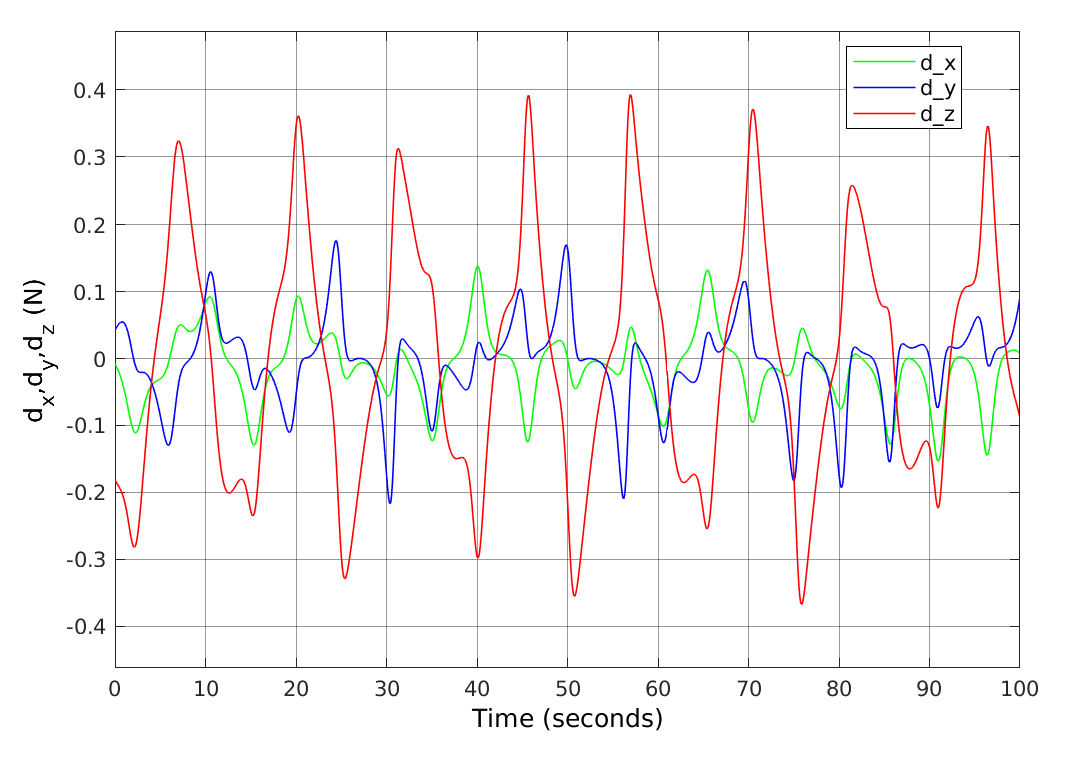
\includegraphics[width=3.5in,height=2in]{Figures/results/chaotic_disturbances/dis_m1_pos.eps}}
\\ \parbox{0.75\textwidth}{\caption{Chaotic Disturbances 1 in Position Subsystem}\label{dis_m1_pos}}
\end{figure}

\begin{figure}[H]
\centering
\fbox{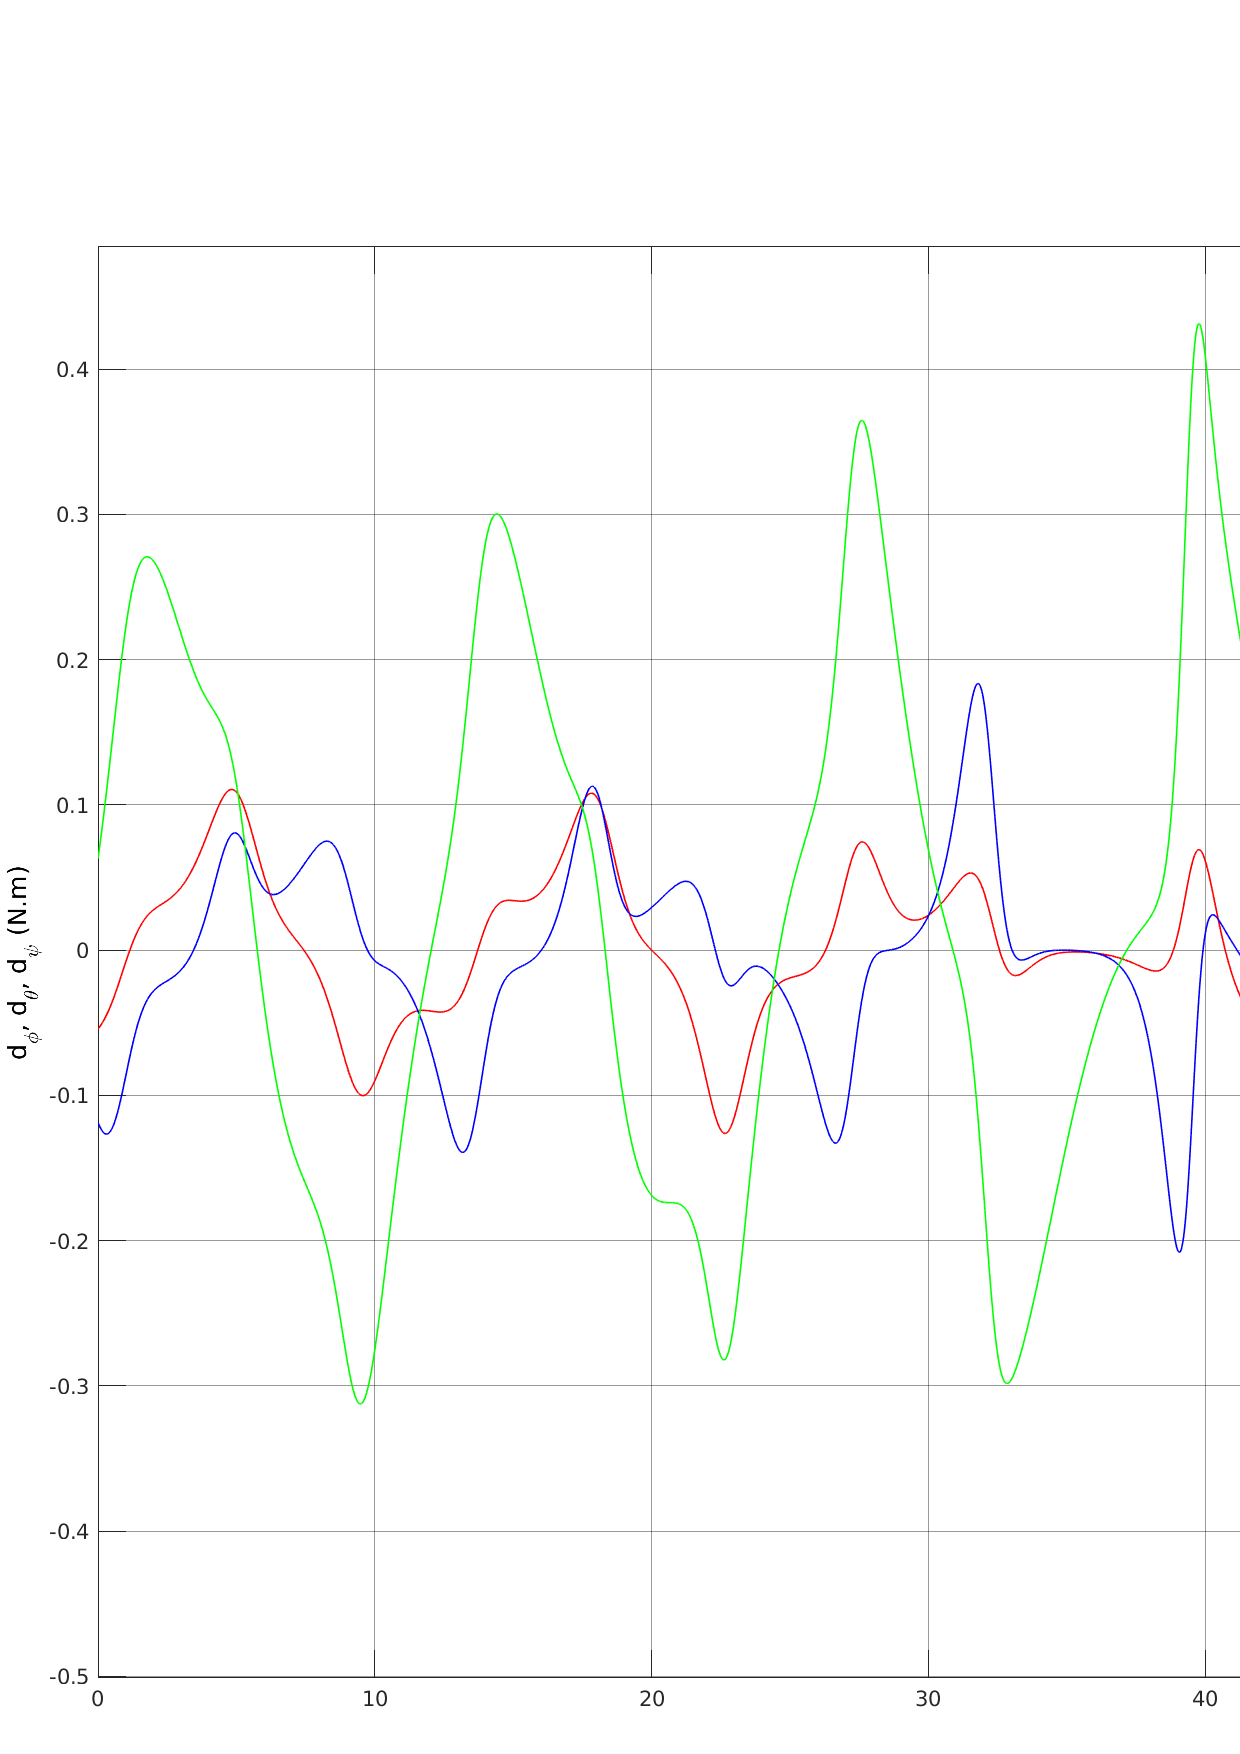
\includegraphics[width=3.5in,height=2in]{Figures/results/chaotic_disturbances/dis_m1_att.png}}
\\ \parbox{0.75\textwidth}{\caption{Chaotic Disturbances 1 in Attitude Subsystem}\label{dis_m1_att}}
\end{figure}


For this set of chaotic disturbances, the estimation results are summarized in Table \ref{Table:SimChaoticRes1}. The convergence time is the time taken by NDO and STO to have an estimation error within the range of $\pm0.1$ when the observers are initialized with the initial observer state of 0.45 for each component. 

\begin{table}[!htbp]
\centering
\caption{Chaotic System 1 \label{Table:SimChaoticRes1}}
\begin{tabular}{|c|c|c|c|c|c|c|}
\hline
{}  &  \multicolumn{2}{c|}{\textbf{NDO}} & \multicolumn{2}{c|}{\textbf{STO}} & \multicolumn{2}{c|}{\textbf{KDO}}\\
\hline
{}        &  \textbf{time}  & \textbf{max err}  & \textbf{time}  & \textbf{max err}& \textbf{time}  & \textbf{max err}\\
$d_z$     &  7.266 & 0.112   & 1.721  & 0.096 & NA     & $8.906*10^{-5}$\\
$d_x$     &  8.201 & 0.147   & 1.659  & 0.090 & NA     & $1.487*10^{-4}$\\
$d_y$     &  4.306 & 0.361   & 3.611  & 0.141 & NA     & $2.401*10^{-4}$\\
$d_\phi$  &  34.08 & 0.110   & 1.902  & 0.041 & NA     & $9.453*10^{-5}$\\
$d_\theta$&  24.52 & 0.183   & 0.650  & 0.089 & NA     & $2.073*10^{-4}$\\
$d_\psi$  &  20.47 & 0.260   & 0.951  & 0.091 & NA     & $1.955*10^{-4}$\\

\hline
\end{tabular}
\end{table}

The cases where the observers estimate the disturbances with the worst performance, is given in Figures \ref{dis_m1_est_yaw_ndo} - \ref{dis_m1_est_yaw_kdo}.

\begin{figure}[H]
\centering
\fbox{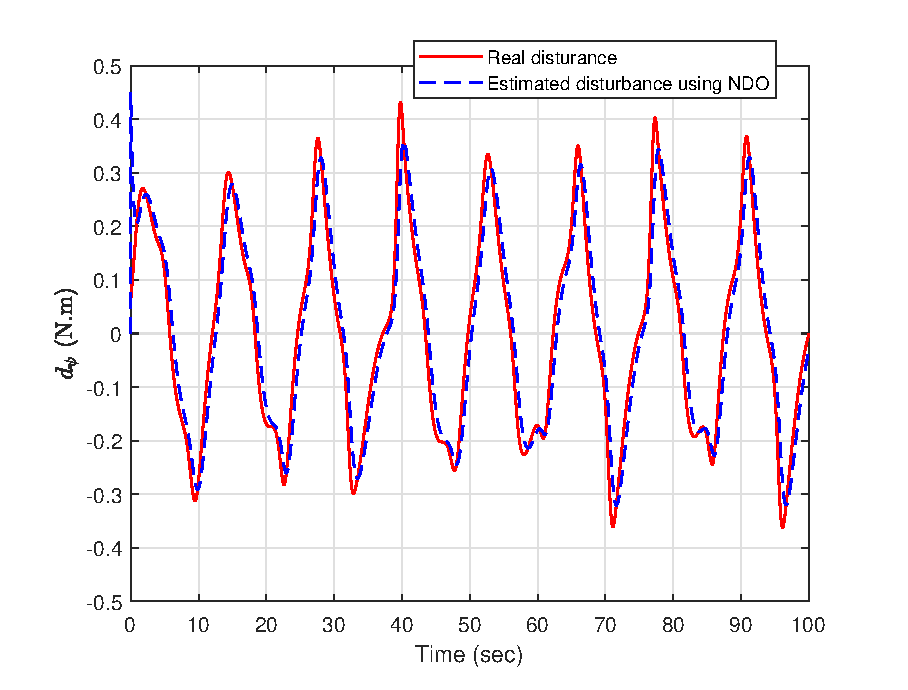
\includegraphics[width=3.5in,height=2in]{Figures/results/chaotic_1_estimates/dis_m1_est_yaw_ndo.eps}}
\\ \parbox{0.75\textwidth}{\caption{Chaotic Disturbances estimation of yaw component using NDO}\label{dis_m1_est_yaw_ndo}}
\end{figure}

\begin{figure}[H]
\centering
\fbox{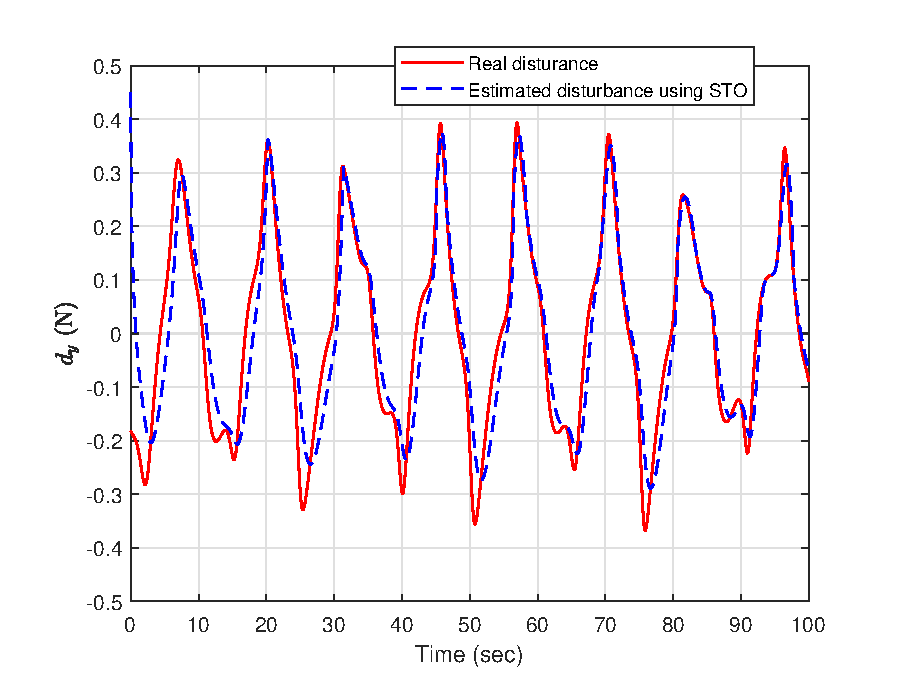
\includegraphics[width=3.5in,height=2in]{Figures/results/chaotic_1_estimates/dis_m1_est_y_sto.eps}}
\\ \parbox{0.75\textwidth}{\caption{Chaotic Disturbances estimation of $y$ component using STO}\label{dis_m1_est_y_sto}}
\end{figure}

\begin{figure}[H]
\centering
\fbox{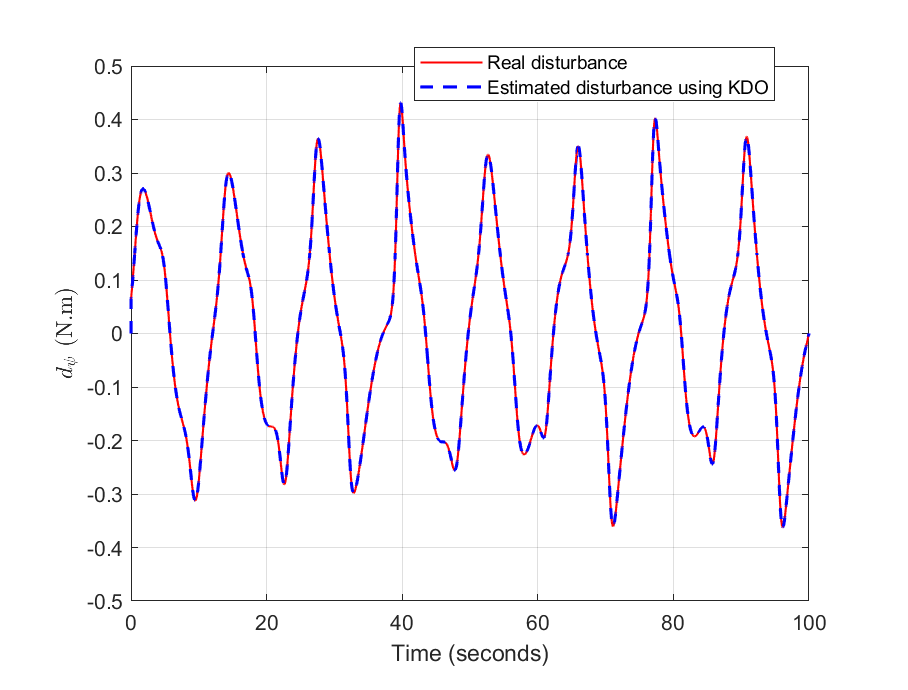
\includegraphics[width=3.5in,height=2in]{Figures/results/chaotic_1_estimates/dis_m1_est_yaw_kdo.eps}}
\\ \parbox{0.75\textwidth}{\caption{Chaotic Disturbances estimation of yaw component using KDO}\label{dis_m1_est_yaw_kdo}}
\end{figure}

It is also observed that among the two chaotic disturbances, the attitude and position tracking performance is worse in this case. The tracking performance is presented in Figures \ref{x_trac_dis_m1_ndo} - \ref{yaw_trac_dis_m1_kdo}: 

\begin{figure}[H]
\centering
\fbox{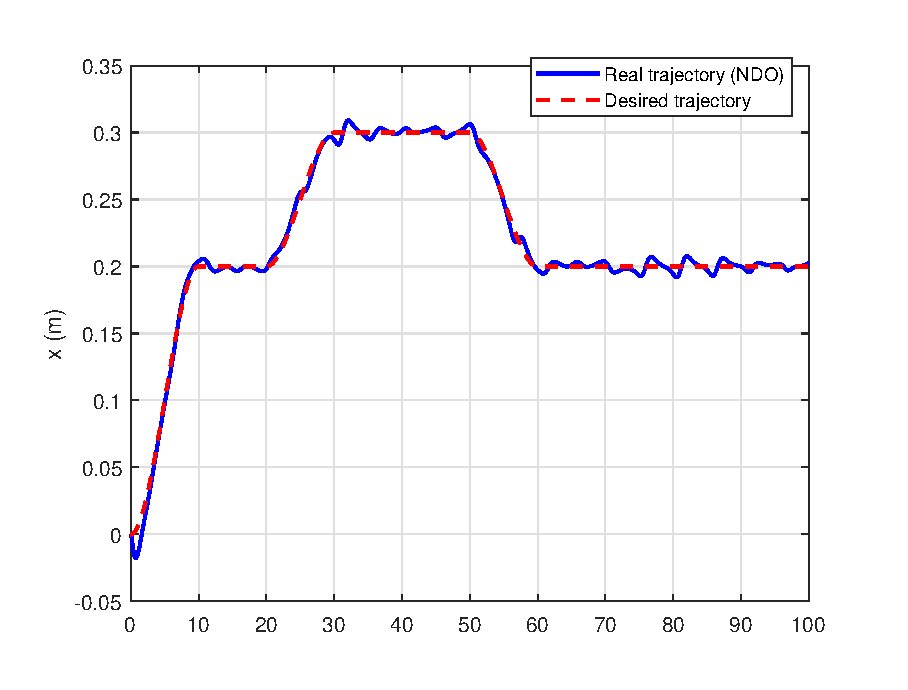
\includegraphics[width=3.5in,height=2in]{Figures/results/tracking/x_trac_dis_m1_ndo.eps}}
\\ \parbox{0.75\textwidth}{\caption{Tracking of $x$ coordinate using NDO}\label{x_trac_dis_m1_ndo}}
\end{figure}

\begin{figure}[H]
\centering
\fbox{\includegraphics[width=3.5in,height=2in]{Figures/results/tracking/x_trac_dis_m1_sto.eps}}
\\ \parbox{0.75\textwidth}{\caption{Tracking of $x$ coordinate using STO}\label{x_trac_dis_m1_sto}}
\end{figure}

\begin{figure}[H]
\centering
\fbox{\includegraphics[width=3.5in,height=2in]{Figures/results/tracking/x_trac_dis_m1_kdo.eps}}
\\ \parbox{0.75\textwidth}{\caption{Tracking of $x$ coordinate using KDO}\label{x_trac_dis_m1_kdo}}
\end{figure}

\begin{figure}[H]
\centering
\fbox{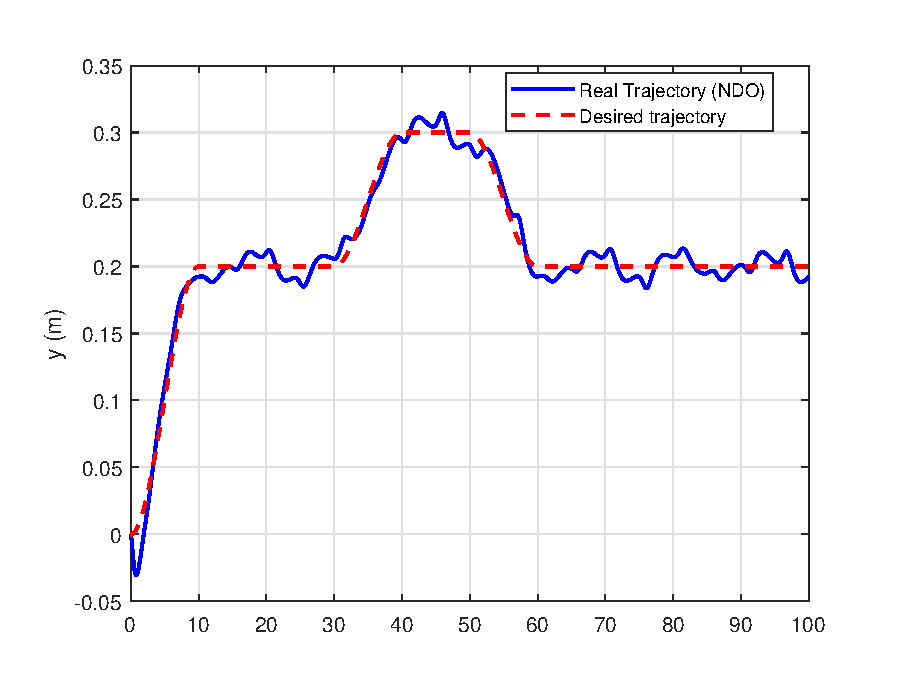
\includegraphics[width=3.5in,height=2in]{Figures/results/tracking/y_trac_dis_m1_ndo.eps}}
\\ \parbox{0.75\textwidth}{\caption{Tracking of $y$ coordinate using NDO}\label{y_trac_dis_m1_ndo}}
\end{figure}

\begin{figure}[H]
\centering
\fbox{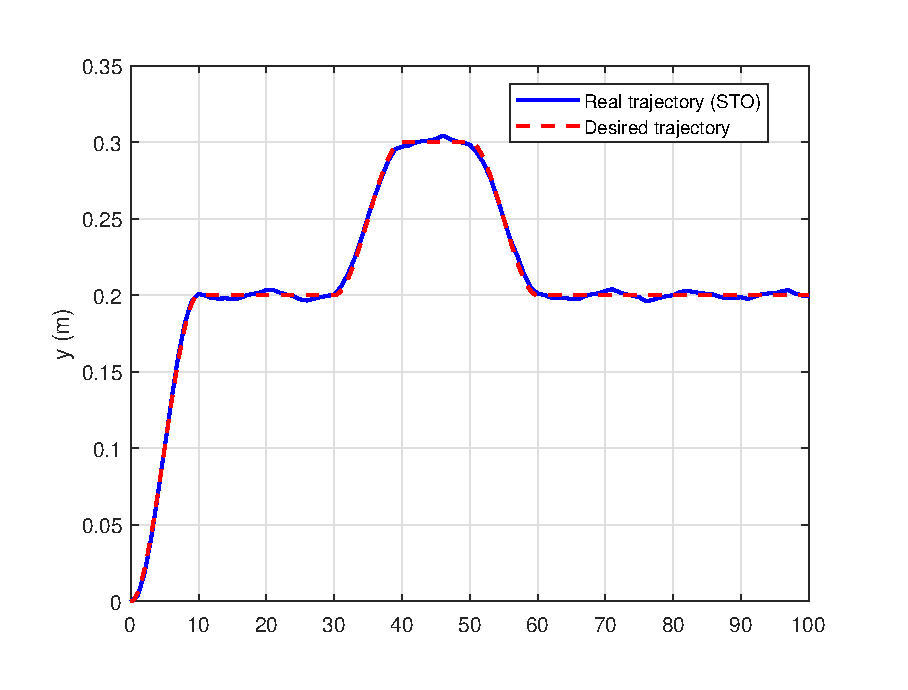
\includegraphics[width=3.5in,height=2in]{Figures/results/tracking/y_trac_dis_m1_sto.eps}}
\\ \parbox{0.75\textwidth}{\caption{Tracking of $y$ coordinate using STO}\label{y_trac_dis_m1_sto}}
\end{figure}

\begin{figure}[H]
\centering
\fbox{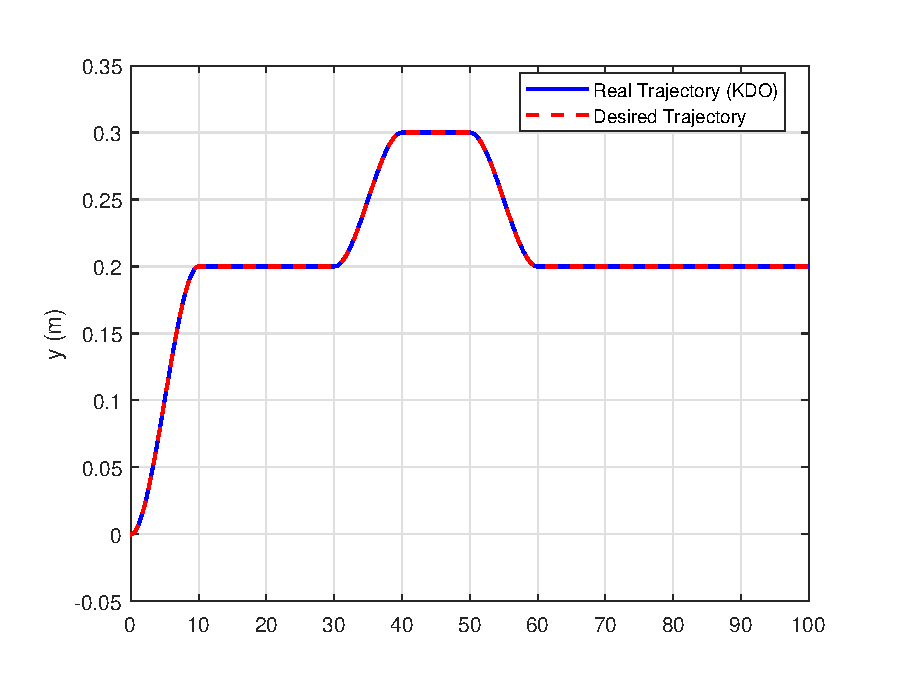
\includegraphics[width=3.5in,height=2in]{Figures/results/tracking/y_trac_dis_m1_kdo.eps}}
\\ \parbox{0.75\textwidth}{\caption{Tracking of $y$ coordinate using KDO}\label{y_trac_dis_m1_kdo}}
\end{figure}

\begin{figure}[H]
\centering
\fbox{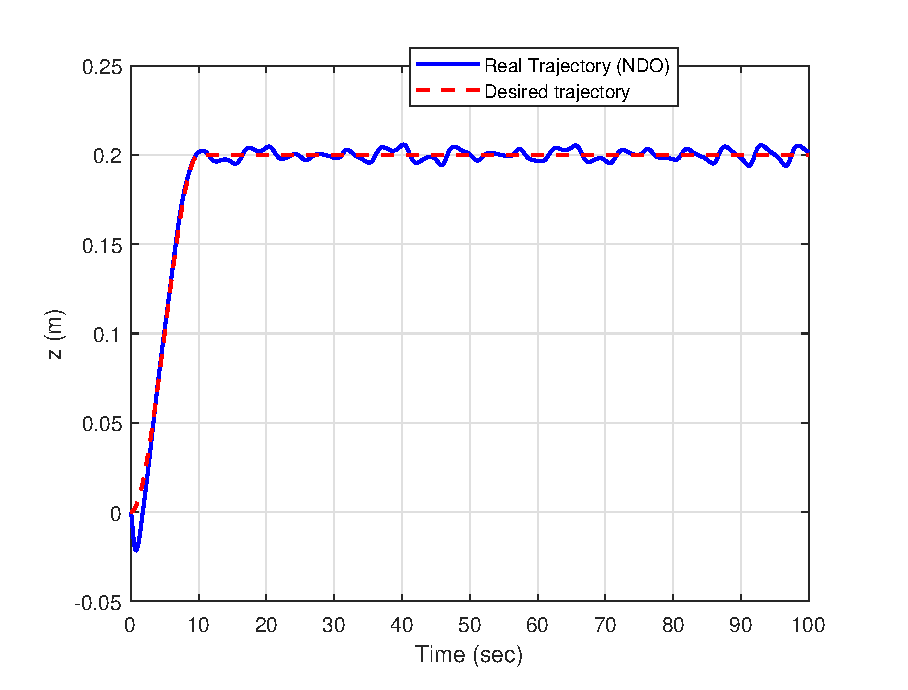
\includegraphics[width=3.5in,height=2in]{Figures/results/tracking/z_trac_dis_m1_ndo.eps}}
\\ \parbox{0.75\textwidth}{\caption{Tracking of $z$ coordinate using NDO}
\label{z_trac_dis_m1_ndo}}
\end{figure}

\begin{figure}[H]
\centering
\fbox{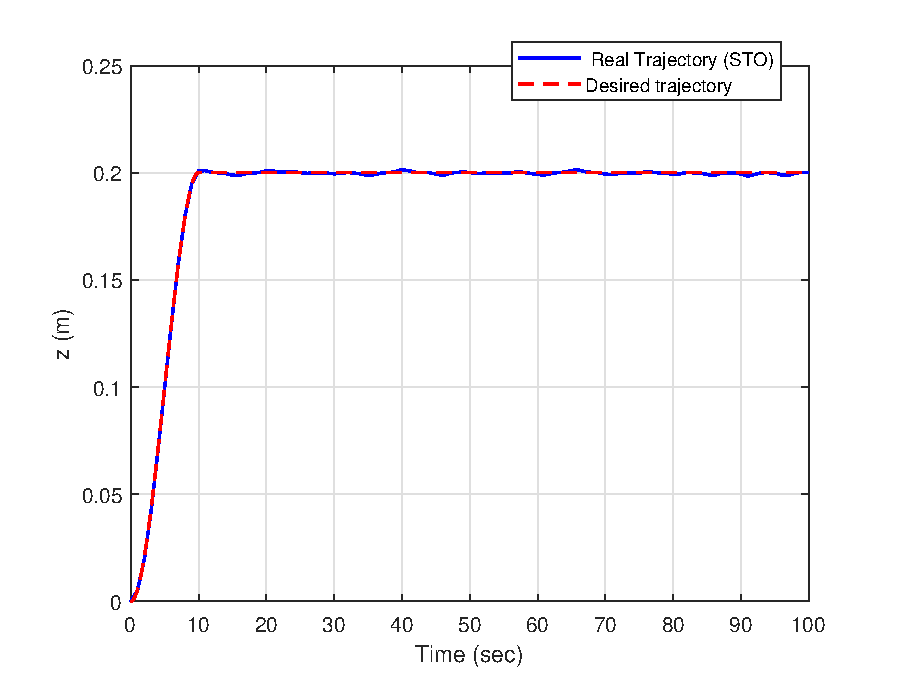
\includegraphics[width=3.5in,height=2in]{Figures/results/tracking/z_trac_dis_m1_sto.eps}}
\\ \parbox{0.75\textwidth}{\caption{Tracking of $z$ coordinate using STO}
\label{z_trac_dis_m1_sto}}
\end{figure}

\begin{figure}[H]
\centering
\fbox{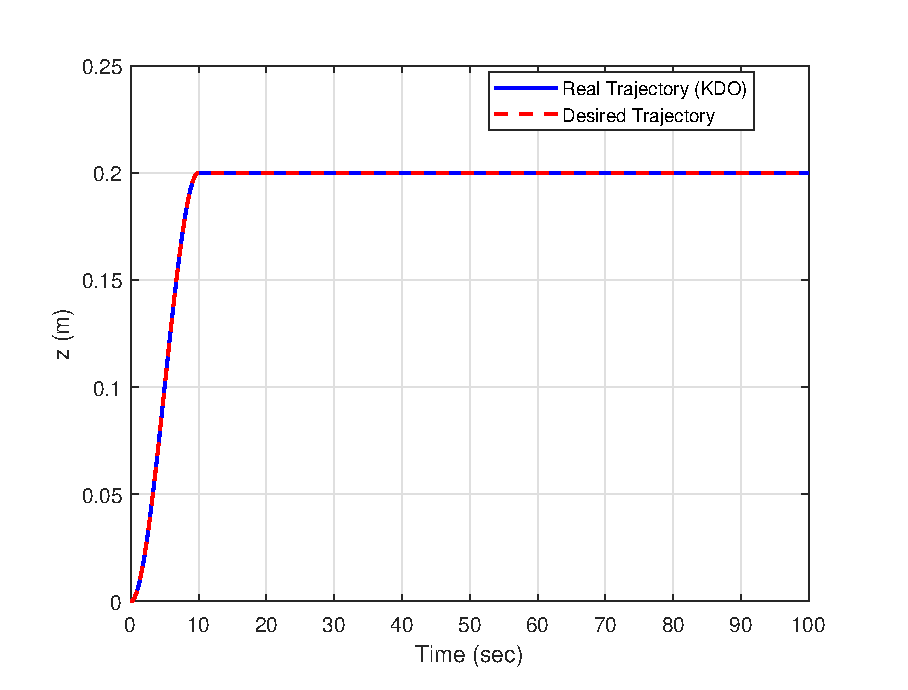
\includegraphics[width=3.5in,height=2in]{Figures/results/tracking/z_trac_dis_m1_kdo.eps}}
\\ \parbox{0.75\textwidth}{\caption{Tracking of $z$ coordinate using KDO}
\label{z_trac_dis_m1_kdo}}
\end{figure}

\begin{figure}[H]
\centering
\fbox{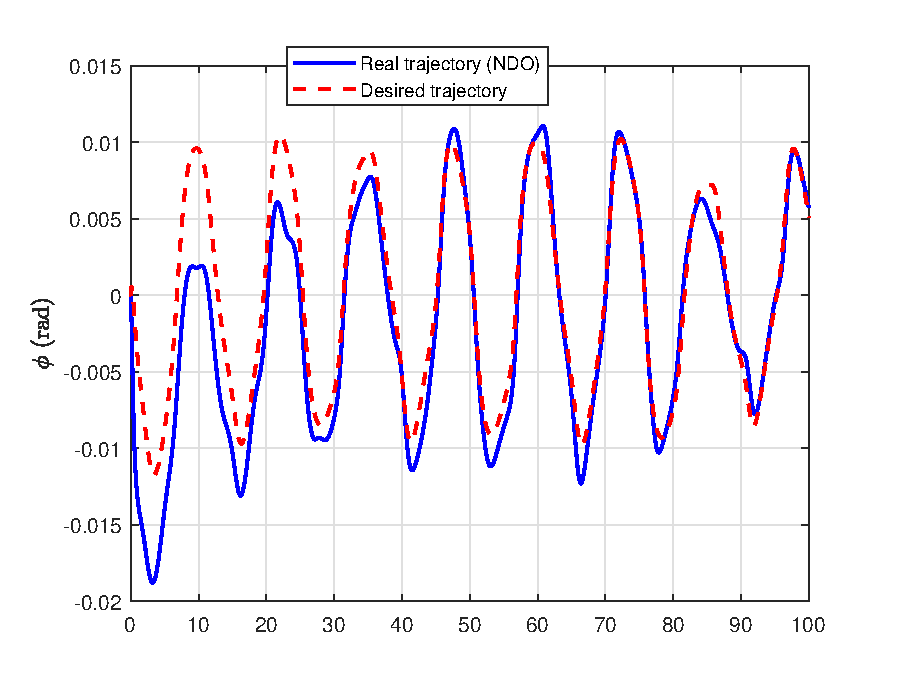
\includegraphics[width=3.5in,height=2in]{Figures/results/tracking/roll_trac_dis_m1_ndo.eps}}
\\ \parbox{0.75\textwidth}{\caption{Tracking of roll angle using NDO}
\label{roll_trac_dis_m1_ndo}}
\end{figure}

\begin{figure}[H]
\centering
\fbox{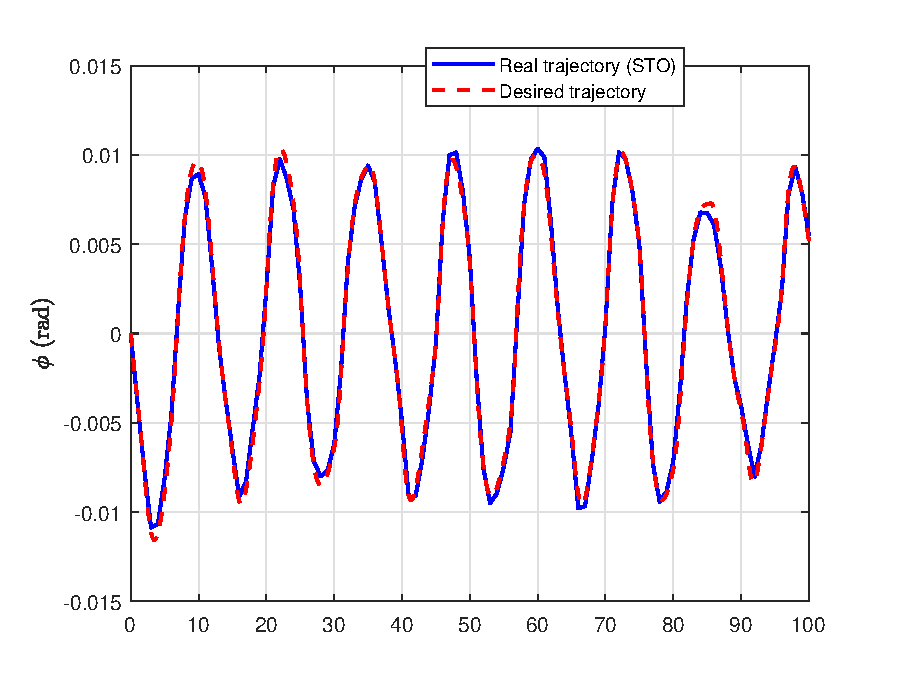
\includegraphics[width=3.5in,height=2in]{Figures/results/tracking/roll_trac_dis_m1_sto.eps}}
\\ \parbox{0.75\textwidth}{\caption{Tracking of roll angle using STO}
\label{roll_trac_dis_m1_sto}}
\end{figure}

\begin{figure}[H]
\centering
\fbox{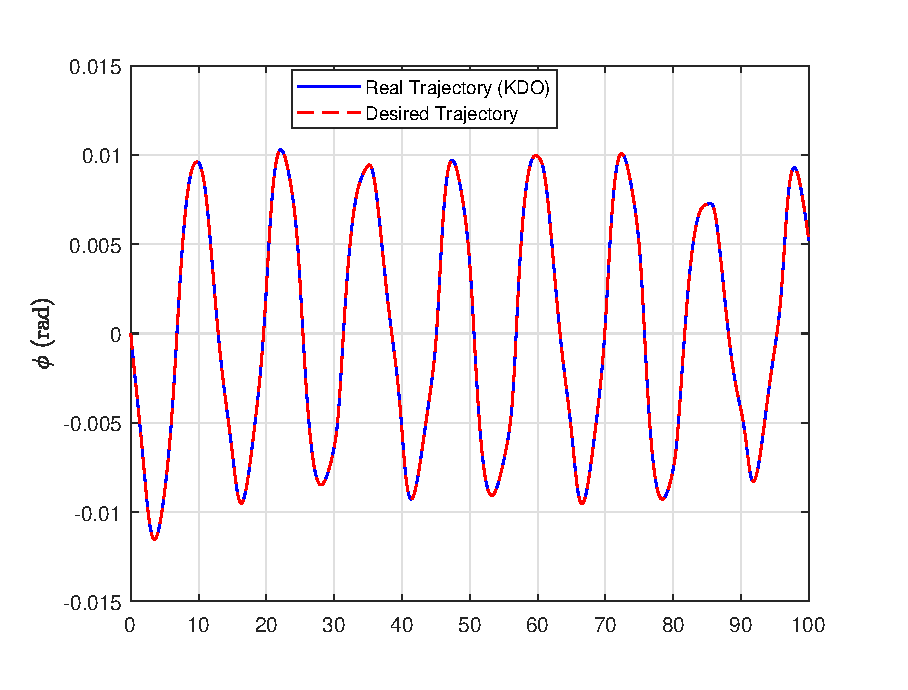
\includegraphics[width=3.5in,height=2in]{Figures/results/tracking/roll_trac_dis_m1_kdo.eps}}
\\ \parbox{0.75\textwidth}{\caption{Tracking of roll angle using KDO}
\label{roll_trac_dis_m1_kdo}}
\end{figure}

\begin{figure}[H]
\centering
\fbox{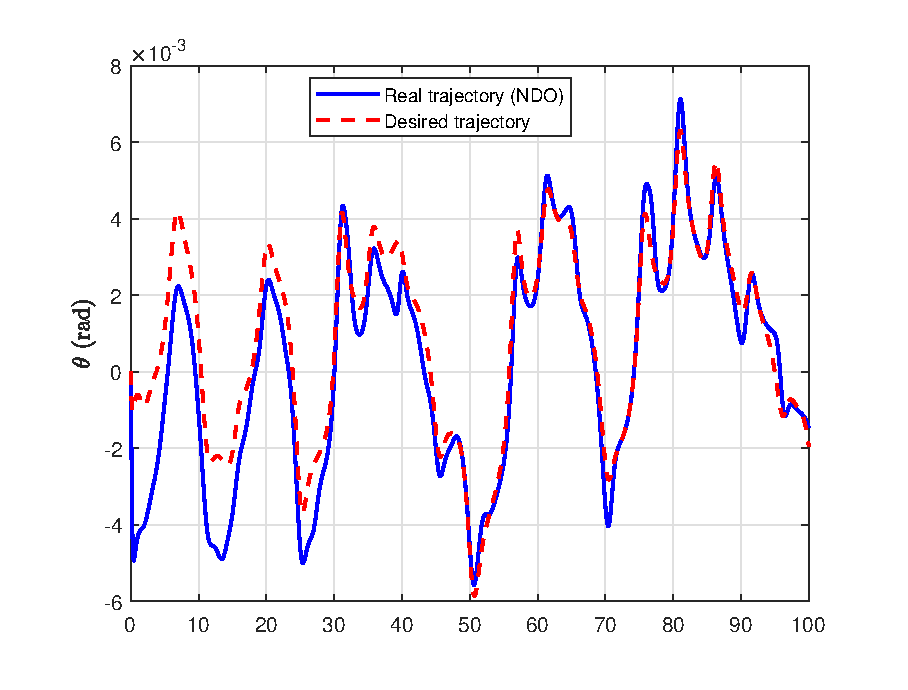
\includegraphics[width=3.5in,height=2in]{Figures/results/tracking/pitch_trac_dis_m1_ndo.eps}}
\\ \parbox{0.75\textwidth}{\caption{Tracking of pitch angle using NDO}
\label{pitch_trac_dis_m1_ndo}}
\end{figure}

\begin{figure}[H]
\centering
\fbox{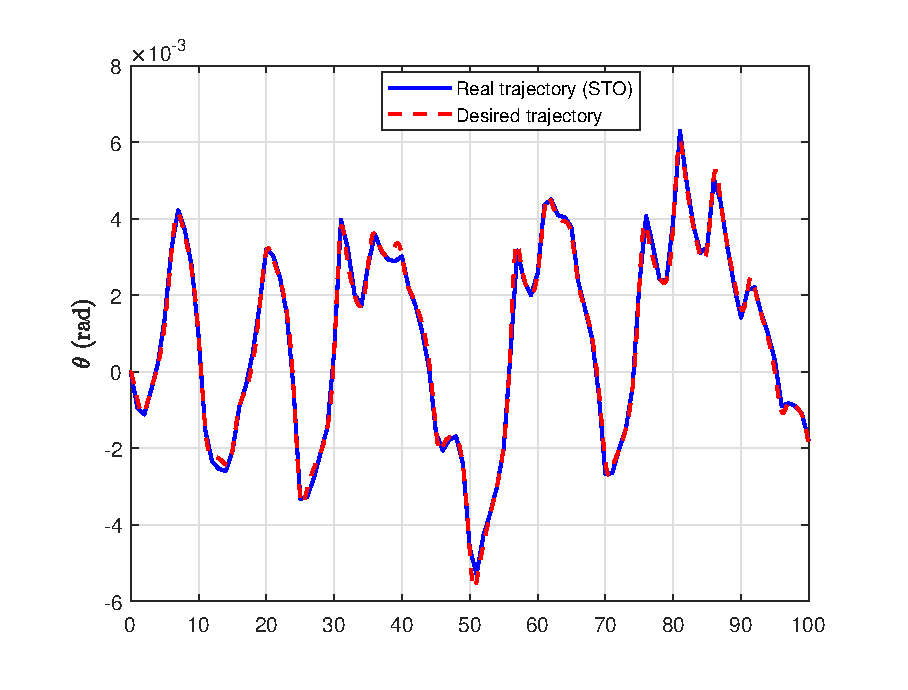
\includegraphics[width=3.5in,height=2in]{Figures/results/tracking/pitch_trac_dis_m1_sto.eps}}
\\ \parbox{0.75\textwidth}{\caption{Tracking of pitch angle using STO}
\label{pitch_trac_dis_m1_sto}}
\end{figure}

\begin{figure}[H]
\centering
\fbox{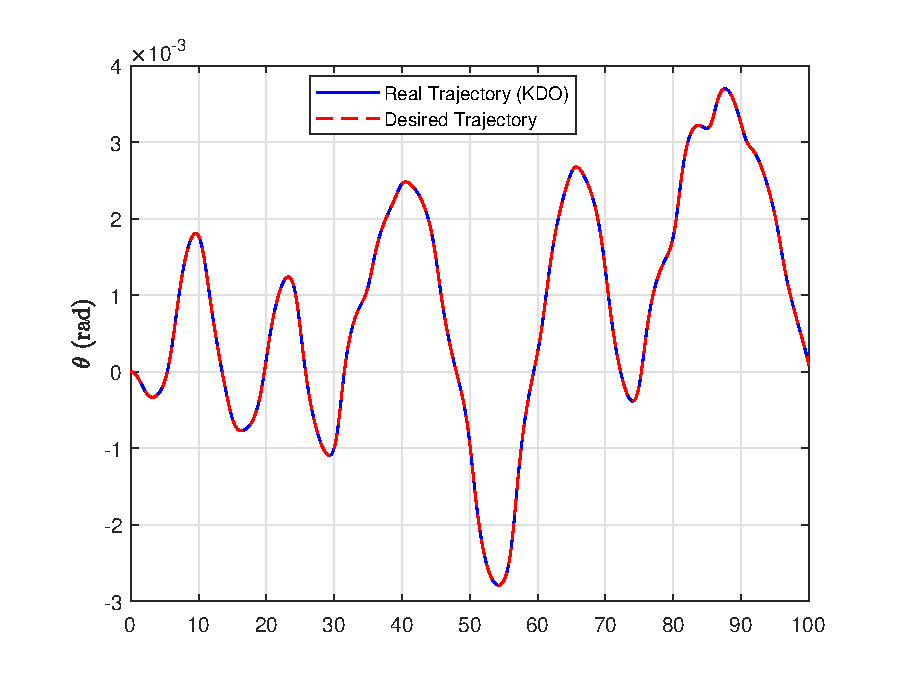
\includegraphics[width=3.5in,height=2in]{Figures/results/tracking/pitch_trac_dis_m1_kdo.eps}}
\\ \parbox{0.75\textwidth}{\caption{Tracking of pitch angle using KDO}
\label{pitch_trac_dis_m1_kdo}}
\end{figure}

\begin{figure}[H]
\centering
\fbox{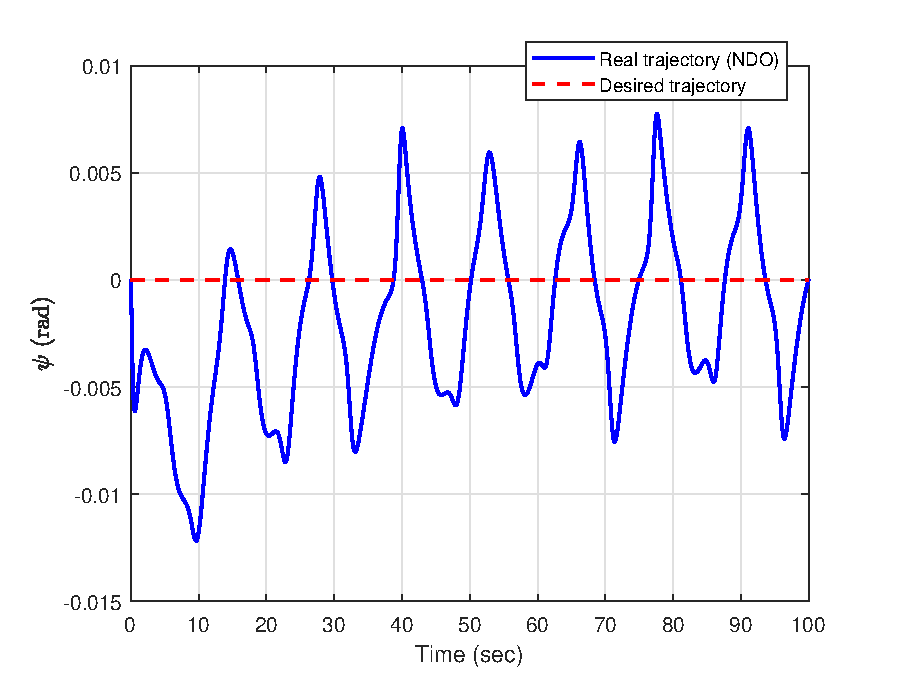
\includegraphics[width=3.5in,height=2in]{Figures/results/tracking/yaw_trac_dis_m1_ndo.eps}}
\\ \parbox{0.75\textwidth}{\caption{Tracking of yaw angle using NDO}
\label{yaw_trac_dis_m1_ndo}}
\end{figure}

\begin{figure}[H]
\centering
\fbox{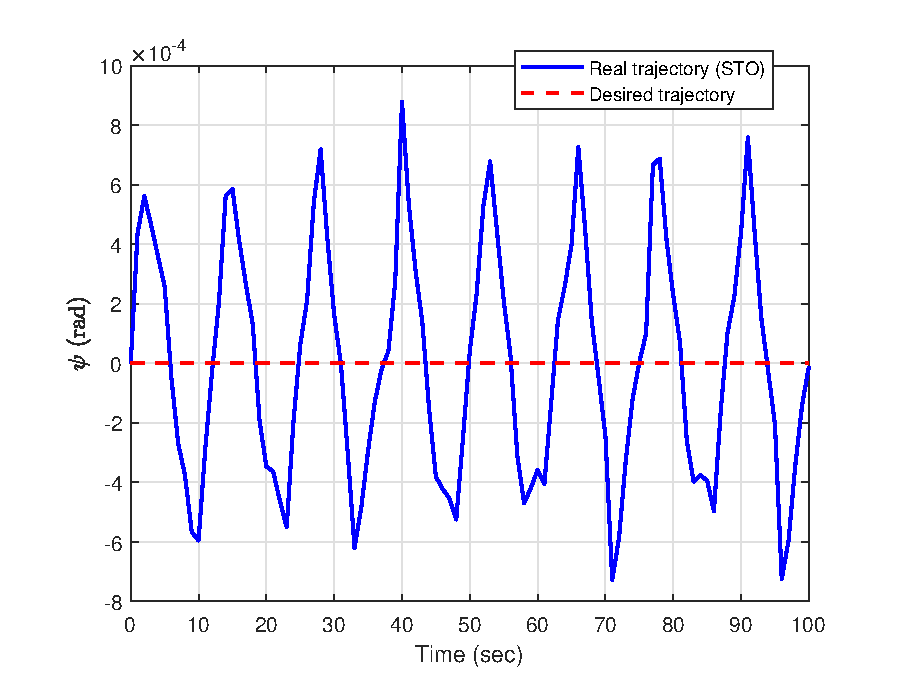
\includegraphics[width=3.5in,height=2in]{Figures/results/tracking/yaw_trac_dis_m1_sto.eps}}
\\ \parbox{0.75\textwidth}{\caption{Tracking of yaw angle using STO}
\label{yaw_trac_dis_m1_sto}}
\end{figure}

\begin{figure}[H]
\centering
\fbox{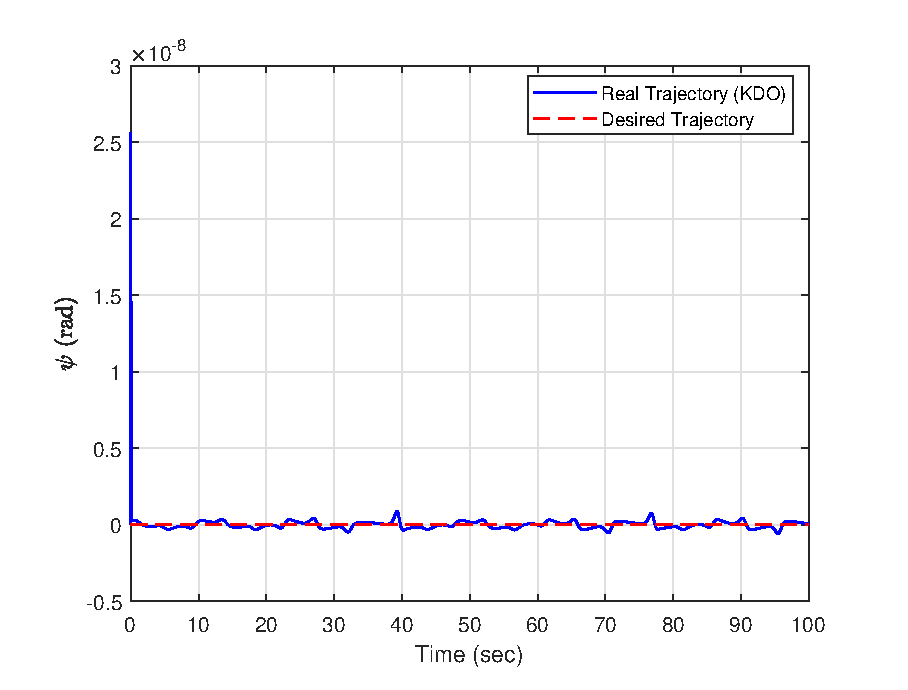
\includegraphics[width=3.5in,height=2in]{Figures/results/tracking/yaw_trac_dis_m1_kdo.eps}}
\\ \parbox{0.75\textwidth}{\caption{Tracking of yaw angle using KDO}
\label{yaw_trac_dis_m1_kdo}}
\end{figure}

\FloatBarrier
\section{Disturbance Model: Chaotic 2}
This section presents results of simulations carried under a chaotic system. The disturbances are again of the form,
\begin{equation}
d_i = k.a_i(t)sin(\omega t-\phi_i)
\label{eq:dist_2}
\end{equation}
where $a_i$ for $i=1...6$, are modeled based on two independent Lorenz chaotic systems $a_i$ for $i=1,2,3$ and the second system for $i=4,5,6$. The system in this case is defined by the set of ordinary equations, 
\begin{subequations}
\begin{align}
a'_1(t) &= 0.1\big(\sigma(a_2-a_1)\big)\\ \nonumber\\
a'_2(t) &= 0.1\big(\rho a_1 - a_1 a_3 - a_2\big)\\ \nonumber \\
a'_3(t) &= 0.1\big(a_1 a_2 - \beta a_3\big)
\end{align}
\end{subequations}
where the constants $\sigma=10$, $\rho=28$, $\beta=\sfrac{8}{3}$, $k=0.0.1$, $\omega=0.5$ with initial values of $a_i$ for $i=1...6$ are given by the vector $[-2,-8,15,-4,-15,20]$, the phase shift values, $\phi_i$ for $i=1...6$ is given by the vector, $[-20,-40-60,-15,-35,-55]$. With this the applied disturbances are non-periodic and chaotic, as seen in Figures \ref{dis_m2_pos} and \ref{dis_m2_att}.

\begin{figure}[H]
\centering
\fbox{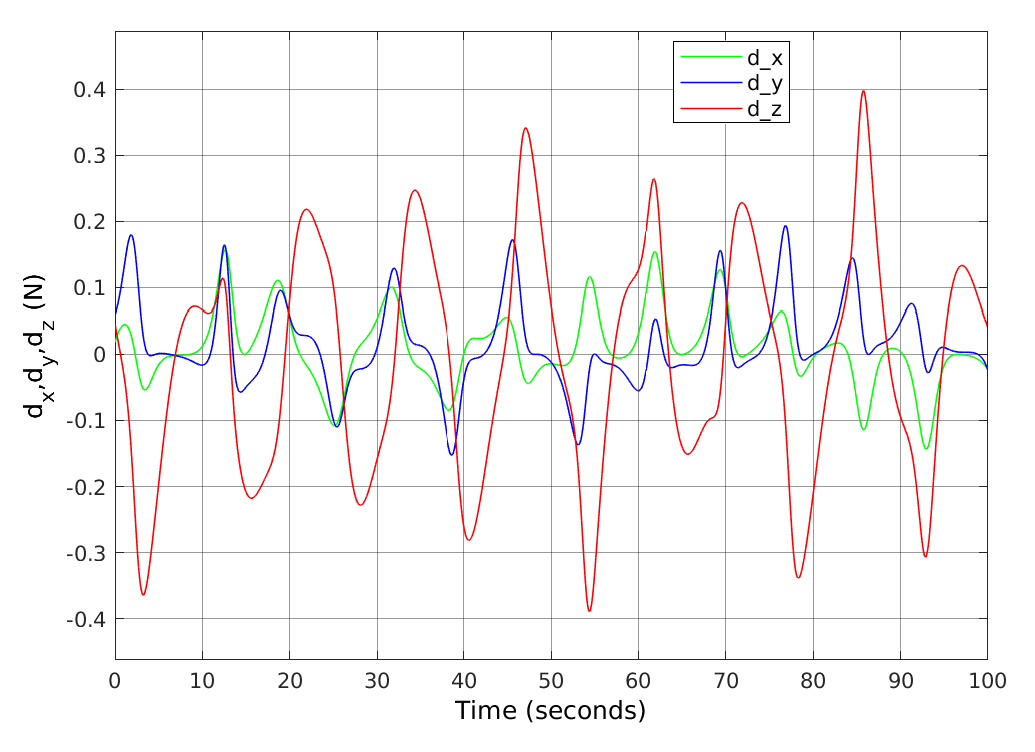
\includegraphics[width=3.5in,height=2in]{Figures/results/chaotic_disturbances/dis_m2_pos.eps}}
\\ \parbox{0.75\textwidth}{\caption{Chaotic Disturbances 2 in Position Subsystem} \label{dis_m2_pos}}
\end{figure}

\begin{figure}[H]
\centering
\fbox{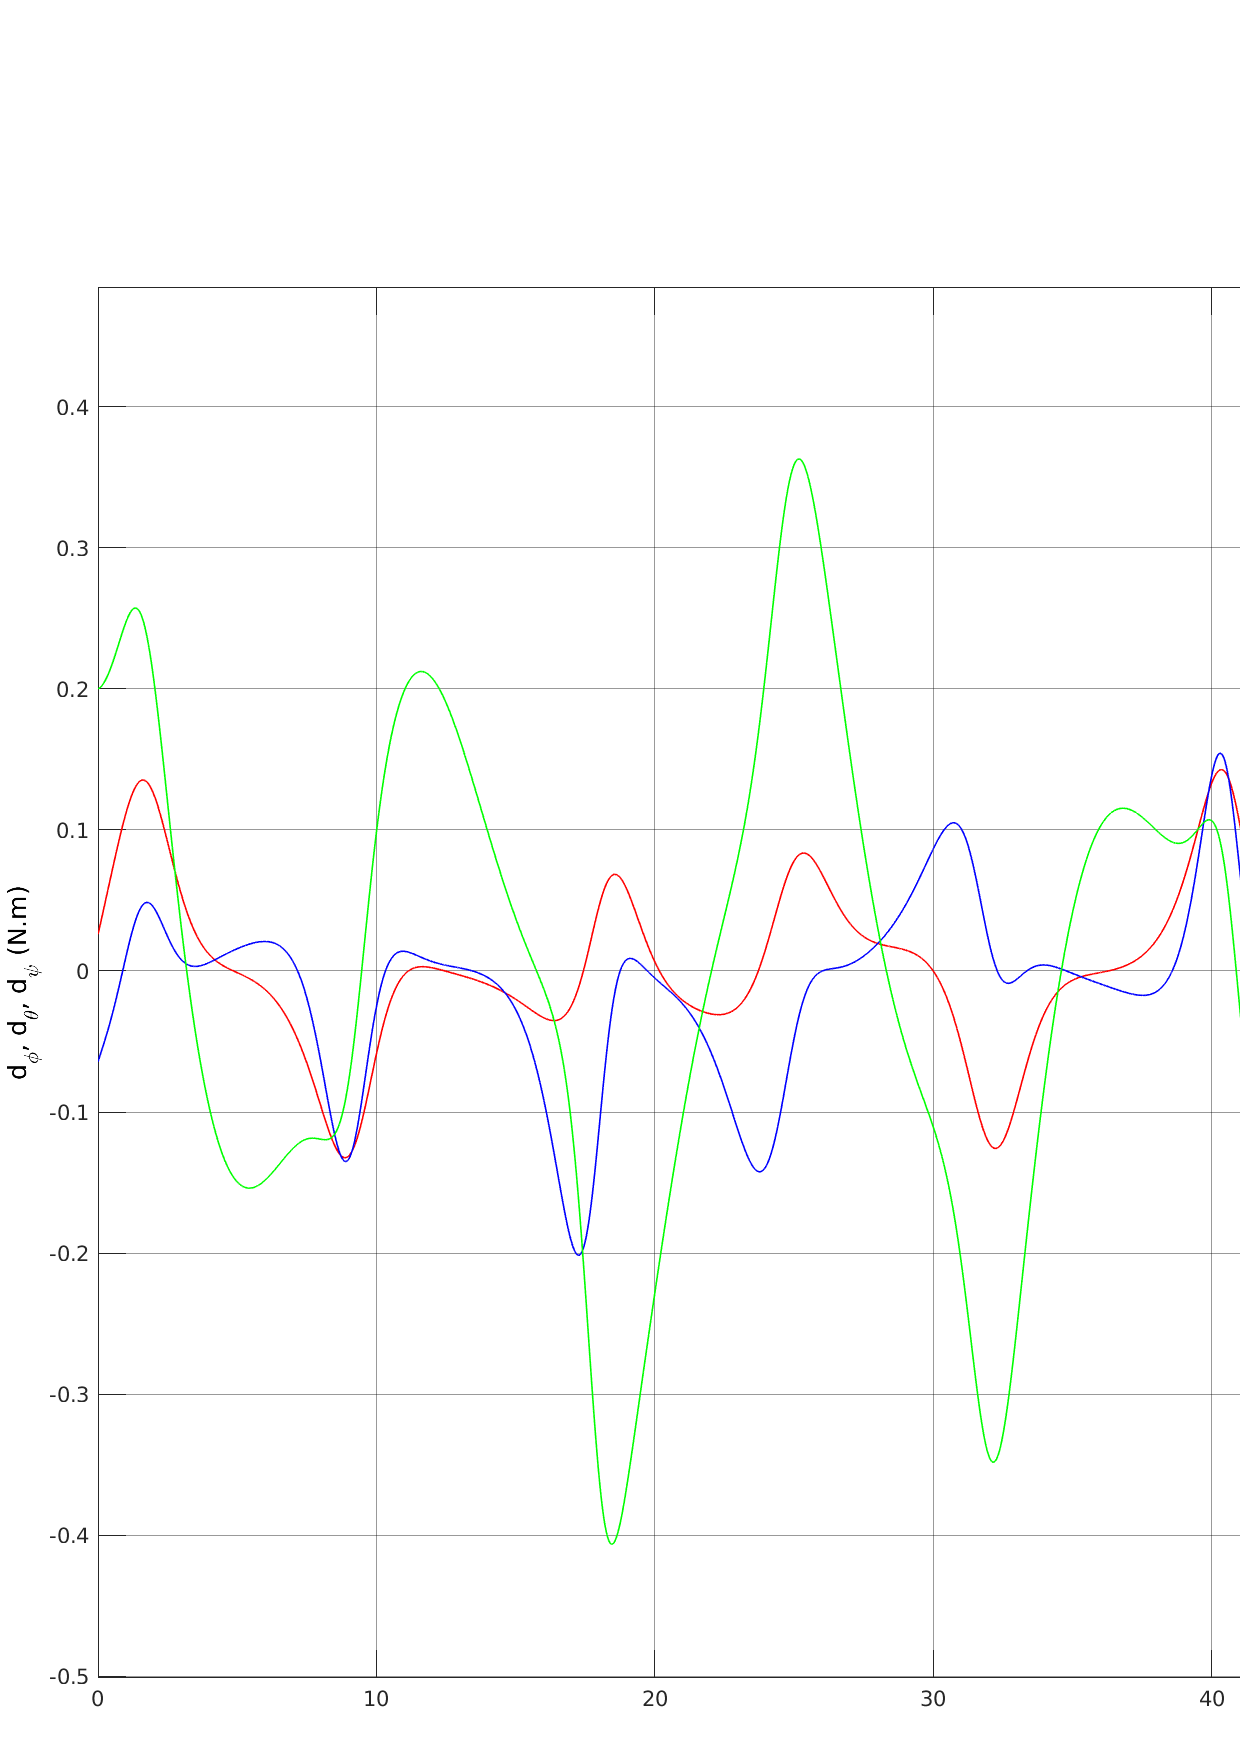
\includegraphics[width=3.5in,height=2in]{Figures/results/chaotic_disturbances/dis_m2_att.png}}
\\ \parbox{0.75\textwidth}{\caption{Chaotic Disturbances 2 in Attitude Subsystem} \label{dis_m2_att}}
\end{figure}

For this set of chaotic disturbances, the estimation results are summarized in Table \ref{Table:SimChaoticRes2}. The convergence time is the time taken by NDO and STO to have an estimation error within the range $\pm0.1$ when the observers are initialized with the initial observer state of 0.45. 

\begin{table}[!htbp]
\centering
\caption{Chaotic System 2 \label{Table:SimChaoticRes2}}
\begin{tabular}{|c|c|c|c|c|c|c|}
\hline
{}  &  \multicolumn{2}{c|}{\textbf{NDO}} & \multicolumn{2}{c|}{\textbf{STO}} & \multicolumn{2}{c|}{\textbf{KDO}}\\
\hline
{}        &  \textbf{time}  & \textbf{max err}  & \textbf{time}  & \textbf{max err}& \textbf{time}  & \textbf{max err}\\
$d_z$     &  6.03 & 0.136   & 3.075  & 0.551 & NA     & $1.422*10^{-4}$\\
$d_x$     &  6.55 & 0.180   & 3.642  & 0.116 & NA     & $3.446*10^{-4}$\\
$d_y$     &  3.12 & 0.388   & 2.289  & 0.136 & NA     & $4.137*10^{-4}$\\
$d_\phi$  &  26.58& 0.155   & 1.204  & 0.025 & NA     & $1.034*10^{-4}$\\
$d_\theta$&  15.82& 0.194   & 1.328  & 0.072 & NA     & $3.575*10^{-4}$\\
$d_\psi$  &  12.34& 0.396   & 2.157  & 0.086 & NA     & $4.893*10^{-4}$\\

\hline
\end{tabular}
\end{table}

The cases where the observers estimate the disturbances with the worst performance, is presented in Figures \ref{dis_m2_est_y_ndo} - \ref{dis_m2_est_y_kdo}.

\begin{figure}[H]
\centering
\fbox{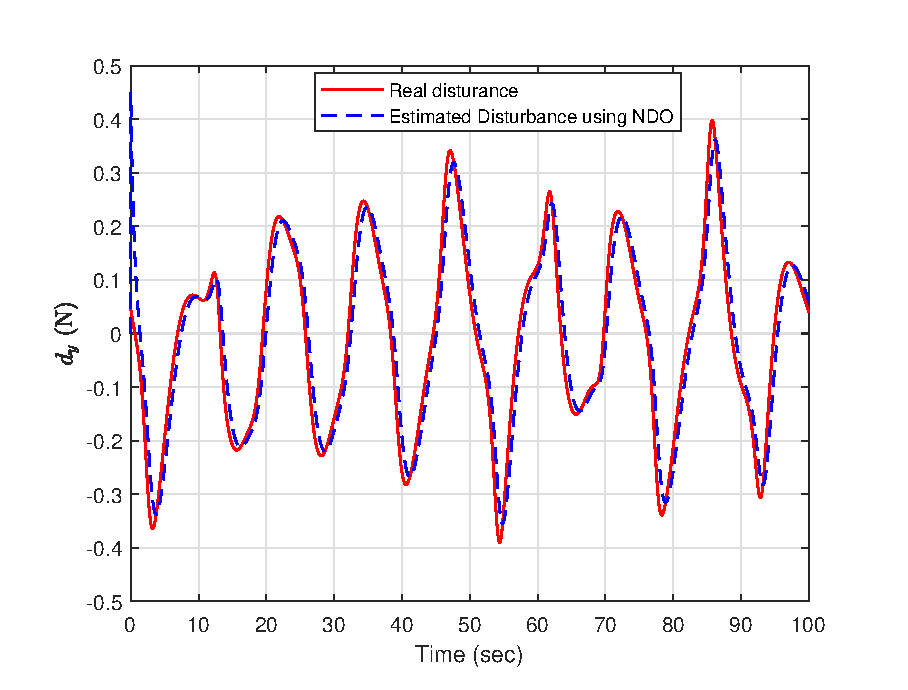
\includegraphics[width=3.5in,height=2in]{Figures/results/chaotic_2_estimates/dis_m2_est_y_ndo.eps}}
\\ \parbox{0.75\textwidth}{\caption{Chaotic Disturbances estimation of $y$ component using NDO} \label{dis_m2_est_y_ndo}}
\end{figure}

\begin{figure}[H]
\centering
\fbox{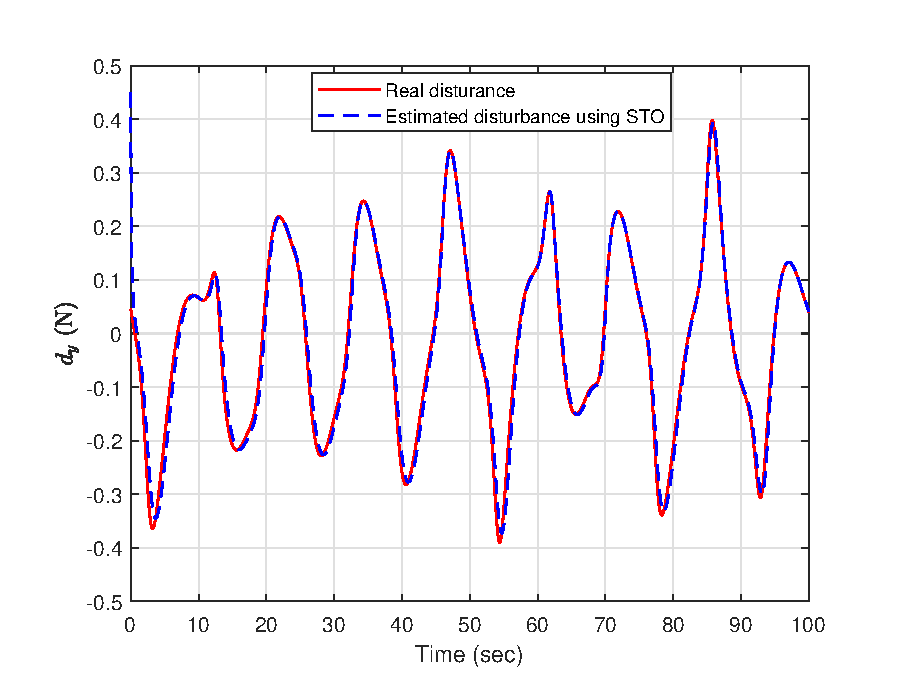
\includegraphics[width=3.5in,height=2in]{Figures/results/chaotic_2_estimates/dis_m2_est_y_sto.eps}}
\\ \parbox{0.75\textwidth}{\caption{Chaotic Disturbances estimation of $y$ component using STO} \label{dis_m2_est_y_sto}}
\end{figure}

\begin{figure}[H]
\centering
\fbox{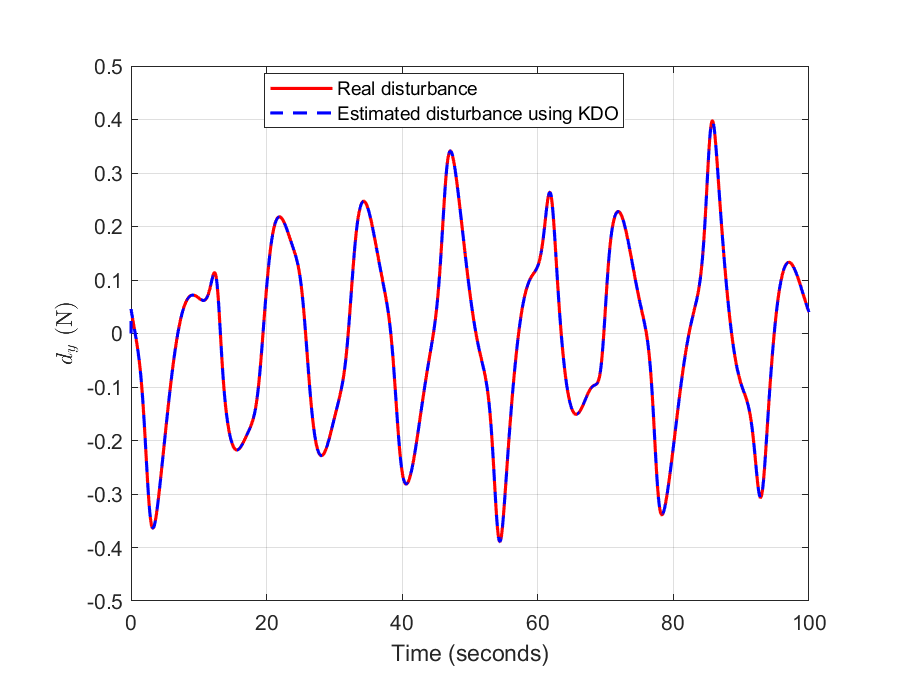
\includegraphics[width=3.5in,height=2in]{Figures/results/chaotic_2_estimates/dis_m2_est_y_kdo.eps}}
\\ \parbox{0.75\textwidth}{\caption{Chaotic Disturbances estimation of $y$ component using KDO} \label{dis_m2_est_y_kdo}}
\end{figure}
%%%%%Blank image inserted
\begin{figure}[H]
	\includegraphics[width=3.5in,height=2in]{Figures/blank.png}
\end{figure}

\FloatBarrier
\section{Disturbance Model: Linear}
The same quadcopter system was also simulated with disturbances that increased or decreased with time. The disturbances were of the form, 
\begin{equation}
d_i = k_i.t
\label{eq:dist_3}
\end{equation}
where the vector $k=[1,-3,2,1.5,2.5,-2.5]*10^{-3}$. 
For the set of linear disturbances the estimation results are summarized in Table \ref{Table:SimLinRes}. The convergence time is the time taken by NDO and STO to have an estimation error within the range $\pm0.1$ when the observers are initialized with the initial observer state of 0.45 for each component. The KDO does not have a convergence time since it is a deadbeat observer unlike NDO and STO which are asymptotic.
\begin{table}[!htbp]
\centering
\caption{Linear Disturbances \label{Table:SimLinRes}}
\begin{tabular}{|c|c|c|c|c|c|c|}
\hline
{}  &  \multicolumn{2}{c|}{\textbf{NDO}} & \multicolumn{2}{c|}{\textbf{STO}} & \multicolumn{2}{c|}{\textbf{KDO}}\\
\hline
{}        &  \textbf{time}  & \textbf{max err}  & \textbf{time}  & \textbf{max err}& \textbf{time}  & \textbf{max err}\\
$d_z$     &  22.757 & 0.005   & 3.549  & 0.0005 & NA     & $1.002*10^{-6}$\\
$d_x$     &  20.254 & 0.015   & 5.204  & 0.0013 & NA     & $3.142*10^{-6}$\\
$d_y$     &  19.584 & 0.001   & 3.420  & 0.0002 & NA     & $2.435*10^{-6}$\\
$d_\phi$  &  55.234 & 0.019   & 2.845  & 0.0006 & NA     & $1.534*10^{-6}$\\
$d_\theta$&  46.565 & 0.045   & 2.594  & 0.0006 & NA     & $2.532*10^{-6}$\\
$d_\psi$  &  41.543 & 0.052   & 2.487  & 0.0005 & NA     & $2.504*10^{-6}$\\
\hline
\end{tabular}
\end{table}

\FloatBarrier
\section{Disturbance Model: Constant}
Similar to the case of applying linear disturbances, linear disturbances were applied to the same quadcopter system where the disturbances remained constant with time. The disturbances were of the form, 
\begin{equation}
d_i = c_i
\label{eq:dist_4}
\end{equation}
where the vector $c=[0.1,0.3,-0.2,-0.05,-0.25,0.15]$. 
For the set of constant disturbances the estimation results are summarized in Table \ref{Table:SimConsRes}. The convergence time is the time taken by NDO and STO to have an estimation error within the range $\pm0.1$ when the observers are initialized with the initial observer state of 0.45 for each component.
\begin{table}[!htbp]
\centering
\caption{Constant Disturbances \label{Table:SimConsRes}}
\begin{tabular}{|c|c|c|c|c|c|c|}
\hline
{}  &  \multicolumn{2}{c|}{\textbf{NDO}} & \multicolumn{2}{c|}{\textbf{STO}} & \multicolumn{2}{c|}{\textbf{KDO}}\\
\hline
{}        &  \textbf{time}  & \textbf{max err}  & \textbf{time}  & \textbf{max err}& \textbf{time}  & \textbf{max err}\\
$d_z$     &  10.354 & 0.359   & 3.259  & 0.359 & NA     & $3.553*10^{-7}$\\
$d_x$     &  10.353 & 0.153   & 2.663  & 0.148 & NA     & $1.735*10^{-7}$\\
$d_y$     &  15.945 & 0.642   & 5.293  & 0.669 & NA     & $2.460*10^{-7}$\\
$d_\phi$  &  25.394 & 0.549   & 3.499  & 0.530 & NA     & $4.163*10^{-7}$\\
$d_\theta$&  26.903 & 0.749   & 5.995  & 0.719 & NA     & $9.702*10^{-7}$\\
$d_\psi$  &  24.959 & 0.392   & 1.639  & 0.344 & NA     & $2.345*10^{-7}$\\
\hline
\end{tabular}
\end{table}


\chapter{Experimental Validation of Observer Based Tracking Control} \label{Chap:ResultsPrac}
The previous section gave insight into how the observers will perform when implemented on an actual quadcopter. The main issue with validating the observer-based tracking control algorithms experimentally is that the actual values of the states being tracked are not innately known, so error in a tracking algorithm can be challenging to measure. In order to validate a tracking algorithm experimentally, a method to accurately measure the state of the quadcopter needed, or methods must be devised to use another measure to compare algorithms. In line with accurately measuring the quadcopter state, the GREPCI Robotics Lab is equipped with a Kinect motion capture system, that provides a very accurate estimate of the position and orientation of the quadcopter during flight. Thus we compare the observers based on the root mean square error in the tracking of the reference trajectory components, i.e. position and yaw. The method of validation has a source of error but provides a reasonable evaluation of the tracking algorithm's performance.The aerodynamic disturbances are induces using the CONAIR 1600 air blower.

\section{Custom Quadcopter setup with Kinect based localization}
In this part we go through the different components of the quadcopter that were chosen to put the system together to meet the computation requirements. \\
\textbf{MAVROS and MAVLink}
ROS (Robot Operating System) is a software framework that provides libraries and visualization and communication tools to streamline the software development of robotic applications. Device drivers, message passing and visualization tools expedite the prototyping process. 
A brief explanation of the different components in the ROS Computation Graph level gives a better understanding of the modifications made to the ROS to expand the message passing between different ROS structures. 

\begin{itemize}
	\item \textbf{Nodes:} Nodes are the computational building blocks of the ROS structure that usually performs computation. Nodes can be written in either C++ or Python. 
	\item \textbf{Messages:} Nodes communicate data packets with each other using messages. ROS provides tools to define custom messages with which are of the form of a C++ data structure. Each ROS package has a \texttt{msg/} subdirectory where custom message descriptions are stored in a \texttt{.msg} file. These message files are simple text files that describe the different fields in the particular ROS message. These help in generating uniform messages through different languages that the ROS framework supports. 
	\item \textbf{Topics:} Topics are strongly typed message bus where messages are routed to nodes that are subscribed to the topic. The messages being published to a topic should be of the appropriate message that is a type defined. This type of publisher/subscriber approach decouples the nodes that produce the information and the one that uses it. 
\end{itemize}
\textbf{MAVLink:} MAVLink is a lightweight messaging protocol for resource-constrained systems. It is used for the ground station computer to communicate with the PIXHAWK drone using the locally setup WiFi. The MAVLink protocol communicates the messages received in the topic \texttt{mavlink/} and then serializes it into an over-the-wire format.\\
\textbf{MAVROS:} MAVROS is a MAVLink extendable communication package that provides the necessary nodes and software for a computer running ROS (or MAVLink enabled ground station computer) to communicate with MAVLink enabled quadcopters. This is especially useful in making distributed computing systems in conjugation with the drone such that the computationally intensive software can run on computers that can execute the computations within the time constraints imposed by a real-time system.\\
\textbf{Custom Message Transmission:} Upon simulation, it was determined that the Kernel computations require much faster hardware to keep up with the time constraints of a real-time system that is susceptible to instability under delayed computations of appropriate control signals. As a result, off-board computation of disturbance estimates from the Kernel Differential Observer was carried out. The computations were done on the same ground station computer that is used to run the computer vision algorithms on the video obtained from the Kinect. The disturbance estimates are then transmitted to the Quadcopter with the MAVLink suite through WiFi.

%\begin{figure}[H]
%\centering
%\fbox{\includegraphics[width=0.85\textwidth]{Figures/theory/rosgraph.eps}}\\
%\parbox{0.75\textwidth}{\caption{ROS computation graph of MAVROS nodes and topics on the ground %station computer\label{rosgraph}}}
%\end{figure}


\textbf{Kinect Setup:} Kinect is a Microsoft product primarily used to give motion sensing capabilities for their gaming consoles range of Xbox. It connects to computing hardware through a USB 3.0 adapter. The Kinect as of date has two versions, V1 and V2, while the project uses the V2 version. The Kinect is an ensemble of two sensors, each serving a different purpose. One is a colour sensor that gives an RGB image of the field of view, whereas the second one is a depth sensor that gives a depth map, which gives a pixel-wise sense of distance of the object from the sensor. OpenNI provides an API to connect to the Kinect and additional capabilities for image manipulation and processing. It gives routines to connect to the Kinect, acquire images and implement matrix manipulation techniques. The quadcopter is fitted with two red balls of different sizes, which help in processing the Kinect data to give the global estimates of the quadcopter position and yaw angle. The red colour of the balls provides a stark contrast to the background and aid in improving the accuracy of estimation.

The estimation algorithm was developed and implemented by a former Graduate student of the lab as a part of his Master's thesis presented in \citep{brice2017thesis}. The estimation algorithm runs on the ground station computer and transmits the global position to the quadcopter via MAVLink, which uses WiFi. The estimate uses a predefined ROS message provided by the MAVROS-MAVLink interface. The nodes \texttt{/kinect2/sd/image\_color\_rect} and \texttt{/kinect2/sd/image\_depth\_rect} estimate the pose and send this estimate to the topic \texttt{/pose\_calculator}. The node \texttt{/mavros/serpoint\_position/local} calculates the local setpoint for the quadcopter for the subsequent iteration and \texttt{/mavros/vision\_pose/pose} calculates the position and the yaw angle of the quadcopter. The estimated pose from Kinect data is taken as the ground truth of the quadcopter state and is used in evaluating the effectiveness and performance of observer-controller tracking algorithms.

\begin{figure}
	\centering
	\fbox{\includegraphics[width=0.75\textwidth]{Figures/practical/quad_red_balls.png}}
	\parbox{0.75\textwidth}{\caption{Quadcopter with the red balls for localization using image processing\label{Fig:quad_red_balls}}}
\end{figure}

\begin{figure}
	\centering
	\fbox{\includegraphics[width=0.75\textwidth]{Figures/practical/quad_flying.png}}
	\parbox{0.75\textwidth}{\caption{Quadcopter during a test flight while using Kinect for attitude estimation\label{Fig:quad_flying}}}
\end{figure}

\underline{The quadcopter hardware primarily contains the following components:}\\
\textbf{Companion Computer:} This is an onboard Linux computer with ROS that connects to a WiFi network that is shared with the ground station computer, which enables the ground station to establish a UDP communication protocol via SSH. For this project, the companion computer used is Odroid XU4. The low weight Odroid XU4 (38g) has Samsung Exynos5422 Cortex-A15 2Ghz and Cortex-A7 Octa core CPUs with 2Gbyte LPDDR3 RAM which can run different versions of Linux and Android. This companion computer also communicates with a flight control board which has integrated motion sensors like accelerometer, gyroscope, magnetometer and barometer. The companion computer requires a companion link to communicate with the flight controller. In this case, the MAVLink suite of communication protocols is used to transmit and receive the data between the companion computer and the flight controller. The flight controller used for this project is Pixhawk 3DR. The two components communicate with FTDI USB breakout and level shifters. 


\begin{figure}[H]
	\centering
	\resizebox{0.75\textwidth}{!}{\fbox{\documentclass{standalone}

\usepackage{tikz}
\usetikzlibrary{shapes,arrows, decorations.markings}

\begin{document}

\tikzstyle{block} = [draw, fill=blue!20, rectangle, 
    minimum height=3em, , align=center]
\tikzstyle{big_arrow} = [decoration={markings,mark=at position 1 with {\arrow[scale=2,>=stealth]{>}}},postaction={decorate}]
\tikzstyle{system} = [draw, fill=green!10, rectangle, rounded corners]
\begin{tikzpicture}
    % Ground Computer Rectangle
    \node [system, minimum width=26em] at (,11) (ground_station) {
    	\begin{minipage}[t][4.3cm]{8cm}\textbf{Ground Station}
    	\end{minipage}
    };
    
    
    % Quadcopter Rectangle
    \node [system, minimum width=15em] at (1,3) (quad) {
    	\begin{minipage}[b][5.5cm]{2cm}\textbf{Quadcopter}
    	\end{minipage}
    };
    	
	% Place all the blocks 
	\node [block] at (,15) (kin) {Windows Xbox Kinect};
    \node [block] at (,12) (ros) {ROS Enabled Computer};
    \node [block] at (4,10) (gc) {qGroundControl};
    \node [block] at (, 7.5) (wifi) {WiFi};
    \node [block] at (, 1.5) (px4) {Flight Control Board\\ (PX4 3DR)};
    \node [block] at (, 3.25) (uart) {UART Adapter};
    \node [block] at (, 5) (odroid) {Companion Computer\\Odroid XU4};
	
	% Draw lines     
    \draw [-] (ros) -- (4,12);
    \draw [-] (4,12) -- (gc);
    
    \draw [-] (gc) -- node [midway] {MAVLink} (4,7.5);
    
    
    \draw [-] (ros) -- (-2,12);
    \draw [-] (-2,12) -- node [midway,] {MAVLink/UDP} (-2,7.5);
	
	% Draw arrows    
    \draw [big_arrow] (4,7.5) --  (wifi);
    \draw [big_arrow] (-2,7.5) -- (wifi);
    \draw [big_arrow] (kin) -- node [above right,] {USB 3.0} (ros);
    
    % Draw arrows in Quadcopter subsystem
	\draw [big_arrow] (wifi) -- (odroid);
    \draw [big_arrow] (odroid) -- (uart);
    \draw [big_arrow] (uart) -- (px4);
    \draw [big_arrow] (kin) -- (ros);
   
   \end{tikzpicture}

\end{document}}}
	\parbox{0.75\textwidth}{\caption{Block diagram of components the distributed computing framework using MAVROS, MAVLink and Windows Xbox Kinect \label{Fig:distributed}}}
\end{figure}

\textbf{Battery:} Quadcopters typically use Lithium Polymer(LiPo), Lithium Polymer High Voltage (LiHV) and Nickel Metal Hydride(NiMH) batteries. This quadcopter uses LiPo batteries. The nominal battery voltage is dependent on the number of cells in the battery. The number of cells and its arrangement is denoted by its 'cell count'. A cell count is a number followed by a letter, where the number indicates the number of cells and the letter indicates the type of arrangement. For example, 3S means there are three cells in series with each other; hence the effective voltage adds up by 3.7V per cell to have an effective voltage of 11.1V. The capacity of the battery is the amount of charge it can hold when fully charged up to its capacity. This usually decreases as the battery is being used. The capacity is indicated in the unit of milliamp-hour (mAh). The capacity of the battery being used is 2250 mAh. Discharge rating is another important rating when choosing the battery. The discharge rating is the rate at which the battery can supply charge safely without adversely affecting the battery. The safe limit current is the product of the discharge rating with the capacity in amperes. For example, the battery used for the quadcopter in testing has the discharge rating 25C and capacity 2250 mAh. The discharge rate is then 25x2.25 = 56.25 A. The battery used for this project is Rhino 2250 3S 25C. 

\begin{figure}[H]
	\centering
	\fbox{\includegraphics[width=0.75\textwidth]{Figures/practical/battery.png}}
	\parbox{0.75\textwidth}{\caption{{Rhino 2250 3S 25C battery with its charger \label{Fig:battery}}}}
\end{figure}
\textbf{Motor Drivers:}Motor drivers act as current and voltage amplifiers. The computer operates in the range of 0-3.3V and voltage of 0-20 mA, where as the motors run on a voltage range of 11.1V and current of 0-60 A. The motor driver used in this project is, Turnigy Multistar 20A V2 ESC With BLHeli and 4A LBEC 2-6S. The motors used are, Multistar Elite 2216 920KV Multirotor Motor (CW).

\FloatBarrier
\section{Computational Implementation}
{\bf Vectorization:} Vectorization refers to Single Instruction Multiple Data operations on several operands in parallel. Most hardware is capable of performing multiple ALU operations simultaneously on data, and instead of running the same operation iteratively using for loops, we can vectorize the operations in terms of matrix computations. Several libraries have optimized code for performing matrix computations and thus, vectorizing code is not only shorter but runs much faster than corresponding loops. In this thesis, we use the GNU Scientific Library (GSL), which provides a stable API for scientific computing which is used for vectorization.
\begin{table}
\parbox{0.65\textwidth}{\caption{Time reductions using vectorization in different programming environments}\label{Tab:vect}}
\begin{tabular}{|c|c|c|c|}
\hline
         & \multicolumn{3}{c|}{\textbf{Programming Language}}\\\cline{2-4} 
\textbf{Time in milliseconds} &   \textbf{MATLAB}   &  \textbf{Python} &   \textbf{C++} \\ \hline
\textbf{Conventional Method}  & 4.082 & 63.3709 & 0.02469    \\
\textbf{Vectorization Method} & 0.553 & 0.0601  & 0.00174    \\
\textbf{Order of Reduction}   & 7.381 & 1054.42 & 14.189     \\
\hline
\end{tabular}
\end{table}
The purpose of representing kernel equations in the form \eqref{eqn:kernVec1} and \eqref{eqn:kernVec2} is to represent the expressions in terms of constant matrices such that vectorized computations would lead to substantial reductions in processing times and thereby satisfy the time constraints posed by real-time systems. The numpy documentation \citep{oliphant2006guide} defines vectorization as, Vectorization describes the absence of any explicit looping, indexing, etc., in the code - these things are taking place, of course, just “behind the scenes” in optimized, pre-compiled C code. Vectorized code has many advantages, among which are:
\begin{itemize}
\item Vectorized code is more concise and easier to read.
\item Fewer lines of code generally means fewer bugs.
\item The code more closely resembles standard mathematical notation (making it easier, typically, to correctly code mathematical constructs).
\item Without vectorization, our code would be littered with inefficient and difficult to read for loops.
\end{itemize}

The double sided kernel method was introduced in \citep{RN76} where the expression for estimate value at a particular instant $t_k$, denoted by $\hat{\zeta}(t_k)$ from the measured value $\zeta_M(t)$ is given by the Equation (\ref{y_E}). 

\begin{equation}\label{y_E}
\hat{\zeta}(t_k) = \int\limits_{a}^{b}K_{DS}(t_k,\tau) \zeta_M(\tau)\, \mathrm{d}\tau
\end{equation}
\begin{equation}
K_{DS}(t_k,\tau) \triangleq \left\{
\begin{array}{lr}
K_{F,\zeta}(t_k,\tau) & for \quad \tau \le t_k\\
K_{B,\zeta}(t_k,\tau) & for \quad \tau > t_k
\end{array}
\right.
\label{K}
\end{equation}
where $K_{F,\zeta}$ and $K_{B,\zeta}$ are given by \eqref{eqn:forward} and \eqref{eqn:backward} respectively. 

At the moment we focus on the Forward Kernel given by \eqref{eqn:forward} This expression is now modified to reduce computational complexities by working under the following assumptions:
\begin{enumerate}
\item A sliding window approach is used
\item Length of the sliding window is fixed i.e. $(b-a)=\textrm{constant}$
\item The relative position of the instant, $(t_k)$,  at which the estimate is to be obtained is fixed with respect to $a\textrm{ and }b \textrm{ i.e. }$ $$ (t_k-a)= a' \textrm{ constant, and } (b-t_k)=b'\textrm{ constant}$$  
\end{enumerate}
Equation \eqref{eqn:forward} is broken down as:
\begin{align} \label{eqn:kernVec1}
K_{F,\zeta}(t,\tau) &\triangleq \quad \frac{1}{[(t_k-a)^4+(b-t_k)^4]} \quad .\nonumber\\
&\begin{bmatrix}
0  &  0  &   0   &  16    &   a_3   \\
0  &  0  &   72   & 12a_3  &   a_2  \\
0  &  96 & 36a_3 &  8a_2  &   a_1   \\
24 &  6  & 12a_2 &  4a_1   &   a_0  
\end{bmatrix}
\begin{bmatrix}
     - 1       \\
 (\tau - a)    \\
-(\tau - a)^2  \\
 (\tau - a)^3  \\
-(\tau - a)^4  \\
\end{bmatrix}
\begin{bmatrix}
1  & (t_k-\tau) & \frac{(t_k-\tau)^2}{2} & \frac{(t_k-\tau)^6}{6}
\end{bmatrix}
\end{align}
\begin{equation} \label{eqn:kernVec2}
= [A][a][t] 
\end{equation}

The matrix $[A]$ depends on the parameters $a_0$, $a_1$, $a_2$, $a_3$. The matrices $[a] \textrm{ and } [t]$ are functions of $(\tau-a) \textrm{ and } (t-\tau)$. These values are then dependent on the relative position in the window. This allows us to calculate the value of the Forward Kernel at each relative point in the window. Once this is computed it need not be computed again. 

\begin{figure}[H]
	\centering
	\resizebox{0.85\textwidth}{!}{\fbox{\documentclass{standalone}

\usepackage{tikz, calc}
\usetikzlibrary{shapes,arrows, decorations.markings}

\begin{document}
\begin{tikzpicture}
	\draw[|-|,semithick] (0,0) -- (10,0);
	\draw[|-,semithick] (5.3,0) -- (3.4,0);
	\draw[|-,semithick] (8.7,0) -- (8.8,0);
	\draw (0,-0.5) node {$a$};
	\draw (10,-0.5) node {$b$};
	\draw (5.3,-0.5) node {$\tau$};
	\draw (8.7,-0.5) node {$t$};
		
	\draw (-2, 0) node {Values};
	\draw[-,dashed] (-1,0.5) -- (-1,-4);
	
	\draw (-2,-1.5) node {$(\tau-a)|^{a}_{t}$};	
	\draw (0,-1.5) node {$0$};	
	\draw (1,-1.5) node {$T$};
	\draw (2,-1.5) node {$2T$};
	\draw (3,-1.5) node {$3T$};
	\draw (8.7,-1.5) node {$(t-a)$};
	
	\draw (-2,-2.5) node {$(t-\tau)|^{a}_{t}$};	
	\draw (0,-2.5) node {$(t-a)$};	
	\draw (3,-2.5) node {$(t-a)-3T$};
	\draw (8.7,-3) node {$0$};
\end{tikzpicture}
\end{document}}}
	\parbox{0.8\textwidth}{\caption{Diagram showing $\tau -a$ and $t-\tau$ remain constant with respect to the position in the sliding window as time progresses \label{sliding_array}}}
\end{figure}

The Forward Kernel as a function of position in sliding window array can be written as:
\begin{align}
K_{F}(i)  &\triangleq \quad \frac{1}{[(t_k-a)^4+(b-t_k)^4]} \quad .\nonumber\\
&\begin{bmatrix}
0  &  0  &   0   &  16    &   a_3   \\
0  &  0  &   72   & 12a_3  &   a_2  \\
0  &  96 & 36a_3 &  8a_2  &   a_1   \\
24 &  6  & 12a_2 &  4a_1   &   a_0  
\end{bmatrix}
\begin{bmatrix}
  -1     \\
 (iT)    \\
-(iT)^2  \\
 (iT)^3  \\
-(iT)^4  \\
\end{bmatrix}
\begin{bmatrix}
1  & \big((n-i)T\big) & \frac{\Big(\big((n-i)T\big)\Big)^2}{2} & \frac{\Big(\big((n-i)T\big)\Big)^3}{6}
\end{bmatrix}
\label{Kfi}
\end{align}
where,
\begin{subequations}
\begin{align}
a+ (\texttt{ number of samples in window * } T)&= b \\ 
a+ (\texttt{t position in window * } T) &= t \\
a+ (\texttt{i}*T) &= \tau
\end{align}
\end{subequations}

The integrand in the forward estimate of $y$ which was previously represented as
$K_F(t,\tau) y_M(\tau)$, 
(in the expression $y_{FE}(t) =\int\limits_{a}^{b}K_F(t,\tau) y_M(\tau)\, \mathrm{d}\tau $ ), 
can be written as 
$$ \vec{y}_{KFM} = [K_F] \textrm{ } \vec{y}_M(i)$$
where 
\begin{equation*}
[K_F] =
\begin{bmatrix}
    K_F(1) &    0   &   0    & \dots  &    0    & \dots  &   0 \\
      0    & K_F(2) &   0    & \dots  &    0    & \dots  &   0 \\
    \vdots & \vdots & \vdots & \ddots & \vdots  & \dots  &   0 \\
      0    &   0    &   0    & \dots  &  K_F(i) & \dots  &   0 \\ 
    \vdots & \vdots & \vdots & \vdots & \vdots  & \ddots &   0 \\
      0    &   0    &   0    & \dots  &    0    & \dots  &   K_F(n) \\
\end{bmatrix}
\end{equation*}
and $K_F(i)$ is given by Equation (\ref{Kfi})

It can be seen that, compared to the previous scheme where the complete Kernel was calculated and derived in each iteration, we just have to compute the Forward Kernel matrix once and then linearly multiply with the incoming measurement vector $\vec{y}_M$ to give the vector $\vec{y}_{KFM}$.
It is hoped that this significant reduction in computation should enable the algorithm to be implemented in real-time. 

The above method can be applied to the Backward Kernel and result in a Double-Sided Kernel Matrix, which is a constant matrix. For the quadcopter, the latency is set to zero to estimate the attitude and orientation of the quadcopter in real-time. While this is not the optimal $t_k$ to minimize estimation variance, setting the latency to a minimum is needed for effective control rather than minimizing the variance. 

\section{Experimental Validation without Disturbances}
The three algorithms were first tested on the quadcopter without any external disturbances. The results for each algorithm are presented in different subsections. The controller gains were tuned by trial and error. The controller gains presented in \citep{RN117} were used as a starting point for tuning. The gains were adjusted in either increments or decrements of 0.1. The gains obtained are presented in individual subsections. 
\subsection{Non-Linear Disturbance Observer Results}
The Non-Linear Disturbance Observer described in Section \ref{Sec:NDO} is implemented on the quadcopter in conjugation with the backstepping and sliding mode controller to track the reference trajectory $[x,y,z,\psi]$ described in \eqref{eqn:x_traj} - \eqref{eqn:z_traj}. Similar to the finding in simulations, the performance of NDO was found to be susceptible to improper tuning of the observer gains. After several iterations the values of gains that gave the best tracking in terms of error and overshoot is presented in Tables \ref{Tab:realNDOGains} and \ref{Tab:realControllerGains}. The figures \ref{Fig:xyztracNDO} - \ref{Fig:3dNDO} show the real flight tracking of the reference trajectory variables, which are the position ($x$, $y$, $z$) and yaw ($\psi$). 
\begin{table}
\parbox{0.65\textwidth}{\caption{Observer gains for NDO}\label{Tab:realNDOGains}}
\begin{tabular}{|c|c|c|c|}
\hline
{\bf Gain}&{\bf Value}&{\bf Gain}&{\bf Value}\\ \hline
$l_x$ & 10 & $l_\theta$  & 10  \\ \hline
$l_y$ & 50 & $l_\phi$    & 10  \\ \hline
$l_z$ & 50 & $l_\psi$    & 10  \\ \hline 
\end{tabular}
\end{table}

\begin{table}
\parbox{0.65\textwidth}{\caption{Controller gains for NDO}\label{Tab:realControllerGains}} 
\begin{tabular}{|c|c|c|c|}
\hline
{\bf Gain} & {\bf Value} & {\bf Gain}         & {\bf Value}  \\ \hline
$k_x$      & 2.2313      & $k_\theta$         & 15           \\ \hline
$k_y$      & 2.2313      & $k_\phi$           & 15           \\ \hline
$k_z$      & 2.116       & $k_\psi$           & 12.961       \\ \hline 
$k_{xx}$   & 0.1313      & $k_{\theta\theta}$ & 12.961       \\ \hline
$k_{yy}$   & 0.1313      & $k_{\phi\phi}$     & 12.961       \\ \hline
$k_{zz}$   & 0.116       & $k_{\psi\psi}$     & 10.961       \\ \hline 
\end{tabular}
\end{table}

\begin{figure}[H]
	\centering
	\fbox{\includegraphics[width=0.85\textwidth]{Figures/results/practical/res1/xyztrac.png}}
	\parbox{0.75\textwidth}{\caption{Real flight tracking of position coordinates using NDO based controller\label{Fig:xyztracNDO}}}
\end{figure}
%%%%%Blank image inserted
\begin{figure}[H]
	\includegraphics[width=0.4\textwidth]{Figures/blank.png}
\end{figure}
\begin{figure}[H]
	\centering
	\fbox{\includegraphics[width=0.75\textwidth]{Figures/results/practical/res1/xyzerr.png}}
	\parbox{0.75\textwidth}{\caption{Position tracking errors using NDO based controller\label{Fig:xyzerrNDO}}}
\end{figure}

\begin{figure}[H]
	\centering
	\fbox{\includegraphics[width=0.75\textwidth]{Figures/results/practical/res1/yaw.png}}
	\parbox{0.85\textwidth}{\caption{Real flight yaw tracking using NDO based controller\label{Fig:yawtracNDO}}}
\end{figure}
The roll and pitch angles are not considered since those values are dynamically dependent on the desired reference trajectory and are not tracked. Due to problems with the battery life, the complete trajectory could not be tracked. Although it should be noted that the part of the trajectory that could not be tracked does not change values and similar results can be expected for the subsequent duration of the flight. \\
The observer was initialized with the initial state of the observer as, $z_p(0)=[2,2,2]$ and $z_\Theta(0)=[4,4,4]$. This incorrect state of the observer was set similar to the simulations to test the real asymptotic nature of the observer. The root-mean-square of the error in tracking is mentioned along with the RMSE of other observers in Section \ref{Sec:PracSumm}.
\begin{figure}[H]
	\centering
	\fbox{\includegraphics[width=0.75\textwidth]{Figures/results/practical/res1/view.png}}
	\parbox{0.85\textwidth}{\caption{Real flight 3D tracking of position using NDO based controller\label{Fig:3dNDO}}}
\end{figure}
%%%%%Blank image inserted
\begin{figure}[H]
	\includegraphics[width=1\textwidth]{Figures/blank.png}
\end{figure}
\FloatBarrier

\subsection{Super-Twisting Observer}
The Super-Twisting Observer described in Section \ref{Sec:STO} is implemented on the quadcopter in conjugation with the backstepping and sliding mode controller to track the reference trajectory $[x,y,z,\psi]$ described in \eqref{eqn:x_traj} - \eqref{eqn:z_traj}. Unlike the NDO, the STO gave similar performance results to reference trajectory tracking for a range of observer gains. The tuning parameters or observer gains that gave the most satisfactory results in terms of overshoot is given in Table \ref{Tab:realSTOGains}. The controller gains used to obtain the results presented here are compiled in Table \ref{Tab:realControllerGainsSTO}. 

\begin{table}
\parbox{0.65\textwidth}{\caption{Observer gains for STO} \label{Tab:realSTOGains}} 
\begin{tabular}{|c|c|c|c|c|c|c|c|}
\hline
{\bf Gain}&{\bf Value}&{\bf Gain}&{\bf Value}&{\bf Gain}&{\bf Value}&{\bf Gain}&{\bf Value}\\ \hline
$\lambda_x$ & 50 & $\lambda_\theta$  & 12  & $\alpha_x$ & 30 & $\alpha_\theta$  & 12  \\ \hline
$\lambda_y$ & 50 & $\lambda_\phi$    & 12  & $\alpha_y$ & 30 & $\alpha_\phi$    & 12  \\ \hline
$\lambda_z$ & 50 & $\lambda_\psi$    & 12  & $\alpha_z$ & 30 & $\alpha_\psi$    & 12  \\ \hline 
\end{tabular}
\end{table}

\begin{table}
\parbox{0.65\textwidth}{\caption{Controller gains for STO}\label{Tab:realControllerGainsSTO}} 
\begin{tabular}{|c|c|c|c|}
\hline
{\bf Gain} & {\bf Value} & {\bf Gain}         & {\bf Value}  \\ \hline
$k_x$      & 2.2313      & $k_\theta$         & 15           \\ \hline
$k_y$      & 2.2313      & $k_\phi$           & 15           \\ \hline
$k_z$      & 2.116       & $k_\psi$           & 12.961       \\ \hline 
$k_{xx}$   & 0.1313      & $k_{\theta\theta}$ & 12.961       \\ \hline
$k_{yy}$   & 0.1313      & $k_{\phi\phi}$     & 12.961       \\ \hline
$k_{zz}$   & 0.116       & $k_{\psi\psi}$     & 10.961       \\ \hline 
\end{tabular}
\end{table}

\begin{figure}[H]
	\centering
	\fbox{\includegraphics[width=0.85\textwidth]{Figures/results/practical/res2/xyztrac.png}}
	\parbox{0.75\textwidth}{\caption{Real flight tracking of position coordinates using STO based controller\label{Fig:xyztracSTO}}}
\end{figure}
%%%%%Blank image inserted
\begin{figure}[H]
	\includegraphics[width=0.35\textwidth]{Figures/blank.png}
\end{figure}
\begin{figure}[H]
	\centering
	\fbox{\includegraphics[width=0.75\textwidth]{Figures/results/practical/res2/xyzerr.png}}
	\parbox{0.75\textwidth}{\caption{Position tracking errors using STO based controller\label{Fig:xyzerrSTO}}}
\end{figure}

\begin{figure}[H]
	\centering
	\fbox{\includegraphics[width=0.65\textwidth]{Figures/results/practical/res2/yaw.png}}
	\parbox{0.65\textwidth}{\caption{Real flight tracking of yaw using STO based controller\label{Fig:yawtracSTO}}}
\end{figure}
\begin{figure}[H]
	\centering
	\fbox{\includegraphics[width=0.75\textwidth]{Figures/results/practical/res2/view.png}}
	\parbox{0.65\textwidth}{\caption{Real flight 3D tracking of position using STO based controller\label{Fig:3dSTO}}}
\end{figure}
%%%% Blank Figure inserted
\begin{figure}[H]
	\includegraphics[width=0.5\textwidth]{Figures/blank.png}
\end{figure}
The roll and pitch angles are not considered since those values are dynamically dependent on the desired reference trajectory and are not tracked. In this experiment, we are able to run the quadcopter for the entire duration of the intended flight time. The observer was initialized with the initial state of the observer as, $\hat{p}(0)=[2,2,2]$ and $\hat{\Theta}(0)=[4,4,4]$. This incorrect state of the observer was set similar to the simulations to test the real asymptotic nature of the observer. The root-mean-square of the error in tracking is mentioned along with the RMSE of other observers in Section \ref{Sec:PracSumm}.

\FloatBarrier
\subsection{Kernel Disturbance Observer}
The Kernel Disturbance Observer described in Chapter \ref{Chap:KDO} is implemented on the quadcopter in conjugation with the backstepping and sliding mode controller to track the reference trajectory $[x,y,z,\psi]$ described in \eqref{eqn:x_traj} - \eqref{eqn:z_traj}. The KDO controller combination gives similar performance results for a variety of controller gains. The controller gains used to obtain the results presented here are compiled in Table \ref{Tab:realControllerGainsKDO}.

\begin{table}
\parbox{0.65\textwidth}{\caption{Controller gains for KDO}\label{Tab:realControllerGainsKDO}} 
\begin{tabular}{|c|c|c|c|}
\hline
{\bf Gain} & {\bf Value} & {\bf Gain}         & {\bf Value}  \\ \hline
$k_x$      & 2.2313      & $k_\theta$         & 15           \\ \hline
$k_y$      & 2.2313      & $k_\phi$           & 15           \\ \hline
$k_z$      & 2.116       & $k_\psi$           & 12.961       \\ \hline 
$k_{xx}$   & 0.1313      & $k_{\theta\theta}$ & 12.961       \\ \hline
$k_{yy}$   & 0.1313      & $k_{\phi\phi}$     & 12.961       \\ \hline
$k_{zz}$   & 0.116       & $k_{\psi\psi}$     & 10.961       \\ \hline 
\end{tabular}
\end{table}

Unlike NDO and STO, the KDO does not have observer gains or tuning parameters. However, the KDO has certain parameters that were kept constant such as the window length and latency in estimation. The window length was of 51 samples, and the latency in estimation was 0s, i.e. the full state was estimated at the time of the latest sample of position and angles. The practical implementation used real-time parameter estimation from kernel expressions by optimizing the least square errors, as shown in Section \ref{Sec:pseudo}. The KDO does not need initial conditions since it is a dead-beat observer. The root-mean-square of the error in tracking is mentioned along with the RMSE of other observers in Section \ref{Sec:PracSumm}.

\begin{figure}[H]
	\centering
	\fbox{\includegraphics[width=0.85\textwidth]{Figures/results/practical/res3/xyztrac.png}}
	\parbox{0.75\textwidth}{\caption{Real flight tracking of position coordinates using KDO based controller\label{Fig:xyztracKDO}}}
\end{figure}
%%%%%Blank image inserted
\begin{figure}[H]
	\includegraphics[width=0.35\textwidth]{Figures/blank.png}
\end{figure}
\begin{figure}[H]
	\centering
	\fbox{\includegraphics[width=0.75\textwidth]{Figures/results/practical/res3/xyzerr.png}}
	\parbox{0.75\textwidth}{\caption{Position tracking errors using KDO based controller\label{Fig:xyzerrKDO}}}
\end{figure}

\begin{figure}[H]
	\centering
	\fbox{\includegraphics[width=0.75\textwidth]{Figures/results/practical/res3/yaw.png}}
	\parbox{0.85\textwidth}{\caption{Real flight tracking of yaw using KDO based controller\label{Fig:yawtracKDO}}}
\end{figure}
\begin{figure}[H]
	\centering
	\fbox{\includegraphics[width=0.75\textwidth]{Figures/results/practical/res3/view.png}}
	\parbox{0.65\textwidth}{\caption{Real flight 3D tracking of position using KDO based controller\label{Fig:3dKDO}}}
\end{figure}
%%%%%Blank image inserted
%\begin{figure}[H]
%	\includegraphics[width=0.3\textwidth]{Figures/blank.png}
%\end{figure}
\FloatBarrier

\section{Experimental Validation with External Disturbances}
The three algorithms were tested on the quadcopter under external disturbances from an air blow dryer. The external disturbances are generated using a CONAIR 1600 air blower. The results for each algorithm are presented in different subsections. The observer and controller gains were kept the same as the gains used under the absence of external disturbances.
\begin{figure}[H]
	\centering
	\fbox{\includegraphics[width=0.75\textwidth]{Figures/dist_pract/dryer.png}}
	\parbox{0.75\textwidth}{\caption{{Quadcopter with the applied disturbances \label{Fig:dryer}}}}
\end{figure}
\subsection{Non-Linear Disturbance Observer Results}
The Non-Linear Disturbance Observer described in Section \ref{Sec:NDO} is implemented on the quadcopter in conjugation with the backstepping and sliding mode controller to track the reference trajectory $[x,y,z,\psi]$ described in \eqref{eqn:x_traj} - \eqref{eqn:z_traj}. The control gains were same ones that were used without external disturbances  presented in Tables \ref{Tab:realNDOGains} and \ref{Tab:realControllerGains}. Figures \ref{Fig:xyztracNDODist} - \ref{Fig:3dNDODist} show the real flight tracking of the reference trajectory variables, which are the position ($x$, $y$, $z$) and yaw ($\psi$). 
\begin{figure}[H]
	\centering
	\fbox{\includegraphics[width=0.75\textwidth]{Figures/dist_pract/res1/xyztrac.png}}
	\parbox{0.75\textwidth}{\caption{Real flight tracking of position coordinates using NDO based controller under external disturbances\label{Fig:xyztracNDODist}}}
\end{figure}

\begin{figure}[H]
	\centering
	\fbox{\includegraphics[width=0.75\textwidth]{Figures/dist_pract/res1/xyzerr.png}}
	\parbox{0.75\textwidth}{\caption{Position tracking errors using NDO based controller under external disturbances\label{Fig:xyzerrNDODist}}}
\end{figure}

\begin{figure}[H]
	\centering
	\fbox{\includegraphics[width=0.7\textwidth]{Figures/dist_pract/res1/yaw.png}}
	\parbox{0.7\textwidth}{\caption{Real flight tracking of yaw using NDO based controller under external disturbances\label{Fig:yawtracNDODist}}}
\end{figure}
\begin{figure}[H]
	\centering
	\fbox{\includegraphics[width=0.7\textwidth]{Figures/dist_pract/res1/view.png}}
	\parbox{0.7\textwidth}{\caption{Real flight 3D tracking of position using NDO based controller under external disturbances\label{Fig:3dNDODist}}}
\end{figure}
%%%%%Blank image inserted
\begin{figure}[H]
	\includegraphics[width=0.9\textwidth]{Figures/blank.png}
\end{figure}
The roll and pitch angles are not considered since those values are dynamically dependent on the desired reference trajectory and are not tracked. Due to problems with the battery life, the complete trajectory could not be tracked. \\
The observer was initialized with the initial state of the observer as, $z_p(0)=[2,2,2]$ and $z_\Theta(0)=[4,4,4]$. This incorrect state of the observer was set similar to the simulations to test the real asymptotic nature of the observer. The root-mean-square of the error in tracking is mentioned along with the RMSE of other observers in a later subsection.
\FloatBarrier

\subsection{Super-Twisting Observer}
The Super-Twisting Observer described in Section \ref{Sec:STO} is implemented on the quadcopter in conjugation with the backstepping and sliding mode controller to track the reference trajectory $[x,y,z,\psi]$ described in \eqref{eqn:x_traj} - \eqref{eqn:z_traj}. The observer and controller gains were the same ones that were used in the case of testing without external disturbances presented in Tables \ref{Tab:realSTOGains} and \ref{Tab:realControllerGainsSTO}. 

\begin{figure}[H]
	\centering
	\fbox{\includegraphics[width=0.85\textwidth]{Figures/dist_pract/res2/xyztrac.png}}
	\parbox{0.75\textwidth}{\caption{Real flight tracking of position coordinates using STO based controller under external disturbances\label{Fig:xyztracSTODist}}}
\end{figure}
%%%%%Blank image inserted
\begin{figure}[H]
	\includegraphics[width=0.1\textwidth]{Figures/blank.png}
\end{figure}
\begin{figure}[H]
	\centering
	\fbox{\includegraphics[width=0.75\textwidth]{Figures/dist_pract/res2/xyzerr.png}}
	\parbox{0.75\textwidth}{\caption{Position tracking errors using STO based controller under external disturbances\label{Fig:xyzerrSTODist}}}
\end{figure}

\begin{figure}[H]
	\centering
	\fbox{\includegraphics[width=0.75\textwidth]{Figures/dist_pract/res2/yaw.png}}
	\parbox{0.75\textwidth}{\caption{Real flight tracking of yaw using STO based controller under external disturbances\label{Fig:yawtracSTODist}}}
\end{figure}
The roll and pitch angles are not considered since those values are dynamically dependent on the desired reference trajectory and are not tracked. In this experiment, we are able to run the quadcopter for the entire duration of the intended flight time. The observer was initialized with the initial state of the observer as, $\hat{p}(0)=[2,2,2]$ and $\hat{\Theta}(0)=[4,4,4]$. This incorrect state of the observer was set similar to the simulations to test the real asymptotic nature of the observer. The root-mean-square of the error in tracking is mentioned along with the RMSE of other observers in Section \ref{Sec:PracSumm}.
\begin{figure}[H]
	\centering
	\fbox{\includegraphics[width=0.75\textwidth]{Figures/dist_pract/res2/view.png}}
	\parbox{0.75\textwidth}{\caption{Real flight 3D tracking of position using STO based controller under external disturbances\label{Fig:3dSTODist}}}
\end{figure}
%%%%%Blank image inserted
\begin{figure}[H]
	\includegraphics[width=0.9\textwidth]{Figures/blank.png}
\end{figure}
\FloatBarrier
\subsection{Kernel Disturbance Observer}
The Kernel Disturbance Observer described in Chapter \ref{Chap:KDO} is implemented on the quadcopter in conjugation with the backstepping and sliding mode controller to track the reference trajectory $[x,y,z,\psi]$ described in \eqref{eqn:x_traj} - \eqref{eqn:z_traj}. The KDO controller combination gives similar performance results for a variety of controller gains. The controller gains were the same ones that were used in the case of testing without external disturbances presented in Table  \ref{Tab:realControllerGainsKDO}.

Unlike NDO and STO, the KDO does not have observer gains or tuning parameters. However, the KDO has certain parameters that were kept constant such as the window length and latency in estimation. The window length was of 51 samples, and the latency in estimation was 0s, i.e. the full state was estimated at the time of the latest sample of position and angles. The practical implementation used real-time parameter estimation from kernel expressions by optimizing the least square errors, as shown in Section \ref{Sec:pseudo}. The KDO does not need initial conditions since it is a dead-beat observer. The root-mean-square of the error in tracking is mentioned along with the RMSE of other observers in Section \ref{Sec:PracSumm}.

\begin{figure}[H]
	\centering
	\fbox{\includegraphics[width=0.75\textwidth]{Figures/dist_pract/res3/xyztrac.png}}
	\parbox{0.85\textwidth}{\caption{Real flight tracking of position coordinates using KDO based controller under external disturbances\label{Fig:xyztracKDODist}}}
\end{figure}
%%%%%Blank image inserted
\begin{figure}[H]
	\includegraphics[width=0.2\textwidth]{Figures/blank.png}
\end{figure}
\begin{figure}[H]
	\centering
	\fbox{\includegraphics[width=0.75\textwidth]{Figures/dist_pract/res3/xyzerr.png}}
	\parbox{0.75\textwidth}{\caption{Position tracking errors using KDO based controller under external disturbances\label{Fig:xyzerrKDODist}}}
\end{figure}

\begin{figure}[H]
	\centering
	\fbox{\includegraphics[width=0.75\textwidth]{Figures/dist_pract/res3/yaw.png}}
	\parbox{0.75\textwidth}{\caption{Real flight tracking of yaw using KDO based controller under external disturbances\label{Fig:yawtracKDODist}}}
\end{figure}
\begin{figure}[H]
	\centering
	\fbox{\includegraphics[width=0.75\textwidth]{Figures/dist_pract/res3/view.png}}
	\parbox{0.75\textwidth}{\caption{Real flight 3D tracking of position using KDO based controller under external disturbances\label{Fig:3dKDODist}}}
\end{figure}
%%%%%Blank image inserted
\begin{figure}[H]
	\includegraphics[width=0.8\textwidth]{Figures/blank.png}
\end{figure}
\FloatBarrier


\section{Summary} \label{Sec:PracSumm}
From the experimental results shown above, it can be seen that the quadcopter is able to track the reference trajectory provided , even in the case of  "external disturbances" experienced in the form of "gusts of wind". The root-mean-square error given by \eqref{eqn:rmse} for the three observers in each of the components of the reference trajectory is tabulated in Table \ref{Tab:rmse} for the case without external disturbances and in Table \ref{Tab:rmseDist} with external disturbances. 

\begin{align}\label{eqn:rmse}
 RMSE = \sqrt{\frac{\Sigma_{i=1}^{n}{\big({d_i -f_i}\big)^2}}{n}}
\end{align}

\begin{table}
\parbox{0.65\textwidth}{\caption{Root Mean Square (RMS) error in each component of reference trajectory tracking by the three observers without external disturbances}\label{Tab:rmse}}
\begin{tabular}{|c|c|c|c|c|}
\hline
         & \multicolumn{4}{c|}{\textbf{Component Reference Trajectory}}\\\cline{2-5} 
\textbf{Observer} &   $x$   &  $y$     &   $z$    & $\psi$  \\ \hline
NDO      & 0.01204 & 0.013824 & 0.02074  & 0.00349 \\
STO      & 0.00471 & 0.00769  & 0.01139   & 0.00324 \\
KDO      & 0.00400 & 0.00574  & 0.011312 & 0.02469 \\
\hline
\end{tabular}
\end{table}

It can be seen that the KDO performs better than NDO and STO in tracking the position and is comparable in tracking the yaw of the quadcopter. However, the KDO does not perform as well as it did in the simulations, and this can be attributed to the measurement noise induced by the sensor. 

\begin{table}
\parbox{0.65\textwidth}{\caption{Root Mean Square (RMS) error in each component of reference trajectory tracking by the three observers under external disturbances}\label{Tab:rmseDist}}
\begin{tabular}{|c|c|c|c|c|}
\hline
         & \multicolumn{4}{c|}{\textbf{Component Reference Trajectory}}\\\cline{2-5} 
\textbf{Observer} &   $x$   &  $y$     &   $z$    & $\psi$  \\ \hline
NDO      & 0.02395 & 0.02045  & 0.04274  & 0.16843 \\
STO      & 0.01048 & 0.01039  & 0.03196  & 0.08538 \\
KDO      & 0.00969 & 0.01096  & 0.02846  & 0.11934 \\
\hline
\end{tabular}
\end{table}

Although implementing KDO over the distributed computing framework is time consuming, it is compensated by the fact that the observer does not have parameters that need to be tuned, unlike NDO and STO. In this light, it can be said that the KDO offers a better practical solution to implementing observer-based tracking controllers in quadcopters as it can be user-friendly to eliminate the need for tuning parameters. Also, this is a first step towards employing kernel methods in real-time systems. 

Since the convergence rates of the asymptotic observers cannot be tested in the practical testing as there is no way to know the external dynamic forces and torques acting, the convergence of the observers was only tested in simulation. It can be seen that improper information of the initial state adversely affects the observer performance but the STO has a faster convergence rate than the NDO. The KDO being a deadbeat observer, gives consistent results over with the estimation error in the similar range throughout the simulation time.

%%- Conclusion -%%
\begin{conclusion}
Controlling systems still remains an important area of research for engineers in the context of modern technology. Control systems rely heavily on the information of the state of the system to compute the control input to have the desired system response. An integral part of this is estimating the external disturbances to a system that usually involves full state estimation, including higher derivatives of the system outputs. Classical methods are still prevalent tools, but there is an increasing interest in the development of dead-beat methods. This thesis explores the properties of these methods in an attempt towards the adaptation of a double-sided kernel-based estimation method in a practical setting of a quadcopter. The introduction chapter gave a brief overview of various approaches in controlling the quadcopter and the recent work done in using observer-based tracking of the quadcopter. There have been advances in the algebraic estimation of differentially flat systems recent publications show that the quadcopter demonstrates these properties. \citep{RN118} uses dynamic ridge regression in a kernel-based approach to trajectory tracking. Although the method is computationally expensive, it does not require any statistical knowledge about the disturbance signals or model uncertainty. 
Chapter 1 introduces the quadcopter model, its flight principle and the dynamics which are useful in simulating the system in SIMULINK. The differential flatness property is discussed in detail with the mathematical definition and an example to provide clarity on the concept. The expressions that exhibit the differential flatness property are also presented.

Chapter 2 discusses the observers between which the trajectory tracking performance is compared. The NDO and STO are presented, and the KDO is developed based on the kernel-based estimation method. Practical Identifiability for a system is described in detail and expressions for fourth-order parameter estimation using minimum least square method are derived. This exact expression is a useful alternative to using dynamic ridge regression to find parameters to the local surrogate models when using kernel methods in systems operating in real-time. 
Chapter 3 uses the presented observers in conjugation with sliding mode control and backstepping control to track the desired trajectory. The comparison in simulation is made under the presence of external aerodynamic disturbances. The NDO and STO were initialized without having the true knowledge of the initial conditions, and convergence rates were measured which wasn't done previously in the literature. The disturbances considered were chaotic, a big change from the smooth sinusoidal disturbances used in simulations previously. The simulations clearly indicate the KDO to have the most accurate estimates of external disturbances that enable better trajectory tracking. It was also noticed that the STO and KDO give similar results to a variety of initial controller gains, while the NDO is sensitive to controller gains and has to be tuned precisely to obtain the desired tracking. The three observers were tested on a quadcopter in real-time and obtained similar results. The KDO was modified to use the exact expressions developed in this thesis to adhere to the computation and time restraints, while the NDO and STO had similar implementations as they did in the simulations and literature. Similar to the simulation results, KDO performed with better tracking of the reference trajectory while STO had comparable performance. However, the NDO fared much worse and was susceptible to the improper tuning of the controller gains. 

The KDO, even after modifications done in this thesis, remains a computationally expensive method. It is recommended that one work towards making the KDO a recursive estimator without having to continuously integrate the whole window but just incorporate the new information and update the state estimate accordingly. This would need the identification of deeper auto-regressive dependencies in the underlying trend of the tracked signal. Such an approach would unavoidably lead to using Bellman's Principle of Optimality in some well-devised Dynamic Programming setting, much resembling the Minimum Energy Estimation as done in \citep{fleming1997deterministic},  \citep{krener2015minimum}. 

Although the MATLAB and Simulink is used for simulations, it is recommended that future simulations using kernel expressions be carried out in C++. Conducting simulations in C++ improves the computation time and makes it possible for rapid continuous development due to speed improvements. GSL provides alternative mathematical routines to the ones found in MATLAB which are used for kernel expression evaluation. ROS Gazebo provides visualization environments for simulations. Physical properties of airflow and dynamics can be imported in the Gazebo environment. This setup would make it efficient integration of algorithms to the firmware for hardware deployment. 

\end{conclusion}



%%%%%%%%%%%%%%%%%%%%%%%%%%%%%%%%%%%%%%%%%%%%%%%%%%%
%  Appendix example:
%%%%%%%%%%%%%%%%%%%%%%%%%%%%%%%%%%%%%%%%%%%%%%%%%%%
\appendix

%% To use more than one appendix
\multiannexe

%% Appendix from an external file
% \include{extApp}

\chapter{Appendix example}


\section{Higher Order Derivatives Expressions} \label{Sec:App1}
Here we present the closed form expressions for the higher derivatives that are too long to me mentioned in the main text. The derivation of these expressions can be found in \citep{RN120}.\\
The closed form expression for $y^{(1)}(t)$ is obtained by adding equations \eqref{eqn:A1} and \eqref{eqn:A2} and dividing by $[(t-a)^{4}+(b-t)^{4}]$.
\begin{equation}\label{eqn:A1}
\begin{split}
	&(t-a)^{(4)}y^{(1)}(t)\\
	&=\bigg[ 12(t-a)^{3}-a_3(t-a)^{4}\bigg]y(t)\\
	&+\int\limits_{a}^{t}\bigg[-72(\tau-a)^{2}+12a_3(\tau-a)^{3}-a_2(\tau-a)^4\bigg]y(\tau)\mathrm{d}\tau\\
	&+\int\limits_{a}^{t}(t-\tau)\bigg[96(\tau-a)-36a_3(\tau-a)^{2}+8a_2(\tau-a)^{3}-a_1(\tau-a)^{4}\bigg]y(\tau)\mathrm{d}\tau\\
	&+\int\limits_{a}^{t}\frac{(t-\tau)^{2}}{2}\bigg[-24+24a_3(\tau-a)-12a_2(\tau-a)^{2}
	\\&\qquad\qquad\qquad{}+4a_1(\tau-a)^{3}-a_0(\tau-a)^{4}\bigg]y(\tau)\mathrm{d}\tau\\
	&+\int\limits_{a}^{t}\frac{(t-\tau)^{2}}{2}(\tau-a)^{4}u(\tau)\mathrm{d}\tau	
\end{split}
\end{equation}
\begin{equation}\label{eqn:A2}
\begin{split}
	&(b-t)^{(4)}y^{(1)}(t)\\
	&=\bigg[-12(b-t)^{3}-a_3(b-t)^{4} \bigg]y(t)\\
	&+\int\limits_{t}^{b}\bigg[72(b-\tau)^{2}+12a_3(b-\tau)^{3}+a_2(b-\tau)^4\bigg]y(\tau)\mathrm{d}\tau\\
	&+\int\limits_{t}^{b}(t-\tau)\bigg[96(b-\tau)+36a_3(b-\tau)^{2}+8a_2(b-\tau)^{3}+a_1(b-\tau)^{4}\bigg]y(\tau)\mathrm{d}\tau\\
	&+\int\limits_{t}^{b}\frac{(t-\tau)^{2}}{2}\bigg[24+24a_3(b-\tau)+12a_2(b-\tau)^{2}
	\\&\qquad\qquad\qquad{}+4a_1(b-\tau)^{3}+a_0(b-\tau)^{4}\bigg]y(\tau)\mathrm{d}\tau\\
	&-\int\limits_{t}^{b}\frac{(t-\tau)^{2}}{2}(b-\tau)^{4}u(\tau)\mathrm{d}\tau	
\end{split}
\end{equation}
The closed form expression for $y^{(2)}(t)$ is obtained by adding equations \eqref{eqn:A3} and \eqref{eqn:A4} and dividing by $[(t-a)^{4}+(b-t)^{4}]$.
\begin{equation}\label{eqn:A3}
\begin{split}
	&(t-a)^{(4)}y^{(2)}(t)\\
	&=\bigg[8(t-a)^{3}-a_3(t-a)^{4}\bigg]y^{(1)}(t)\\&+\bigg[36(t-a)^{2}+8a_3(t-a)^{3}-a_2(t-a)^{4}\bigg]y(t)\\
	&+\int\limits_{a}^{t}\bigg[96(\tau-a)-36a_3(\tau-a)^{2}+8a_2(\tau-a)^{3}-a_1(\tau-a)^{4}\bigg]y(\tau)\mathrm{d}\tau\\
	&+\int\limits_{a}^{t}(t-\tau)\bigg[-24+24a_3(\tau-a)-12a_2(\tau-a)^{2}
	\\&\qquad\qquad\qquad{}+4a_1(\tau-a)^{3}-a_0(\tau-a)^{4}\bigg]y(\tau)\mathrm{d}\tau\\
	&+(t-\tau)(\tau-a)^{4}u(\tau)\mathrm{d}\tau
\end{split}
\end{equation}
\begin{equation}\label{eqn:A4}
\begin{split}
	&(b-t)^{(4)}y^{(2)}(t)\\
	&=\bigg[-8(b-t)^{3}-a_3(b-t)^{4}\bigg]y^{(1)}(t)\\&+\bigg[-36(b-t)^{2}-8a_3(b-t)^{3}-a_2(b-t)^{4}\bigg]y(t)\\
	&+\int\limits_{t}^{b}\bigg[96(b-\tau)+36a_3(b-\tau)^{2}+8a_2(b-\tau)^{3}+a_1(b-\tau)^{4}\bigg]y(\tau)\mathrm{d}\tau\\
	&+\int\limits_{t}^{b}(t-\tau)\bigg[24+24a_3(b-\tau)+12a_2(b-\tau)^{2}
	\\&\qquad\qquad\qquad{}+4a_1(b-\tau)^{3}+a_0(b-\tau)^{4}\bigg]y(\tau)\mathrm{d}\tau\\
	&-(t-\tau)(b-\tau)^{4}u(\tau)\mathrm{d}\tau
\end{split}
\end{equation}
The closed form expression for $y^{(3)}(t)$ is obtained by adding equations \eqref{eqn:A5} and \eqref{eqn:A6} and dividing by the term $[(t-a)^{4}+(b-t)^{4}]$.
\begin{equation}\label{eqn:A5}
\begin{split}
	&(t-a)^{(4)}y^{(3)}(t)\\
	&=\bigg[4(t-a)^{3} - a_3(t-a)^{4}\bigg]y^{(2)}(t)\\
	&+\bigg[-12(t-a)^{2}+4a_3(t-a)^{3}-a_2(t-a)^{4}\bigg]y^{(1)}(t)\\
	&+\bigg[24(t-a)-12a_3(t-a)^{2}+4a_2(t-a)^{3}-a_1(t-a)^{4}\bigg]y(t)\\
	&+\int\limits_{a}^{t}\bigg[-24+24a_3(\tau-a)-12a_2(\tau-a)^{2}+4a_1(\tau-a)^{3}-a_0(\tau-a)^{4}\bigg]y(\tau)\mathrm{d}\tau\\
	&+\int\limits_{a}^{t}(\tau-a)^{4}u(\tau)\mathrm{d}\tau
\end{split}
\end{equation}
\begin{equation}\label{eqn:A6}
\begin{split}
	&(b-t)^{(4)}y^{(3)}(t)\\
	&=\bigg[-4(b-t)^{3} - a_3(b-t)^{4}\bigg]y^{(2)}(t)\\
	&+\bigg[-12(b-t)^{2}-4a_3(b-t)^{3}-a_2(b-t)^{4}\bigg]y^{(1)}(t)\\
	&+\bigg[-24(b-t)-12a_3(b-t)^{2}-4a_2(b-t)^{3}-a_1(b-t)^{4}\bigg]y(t)\\
	&+\int\limits_{t}^{b}\bigg[24+24a_3(b-\tau)+12a_2(b-\tau)^{2}+4a_1(b-\tau)^{3}+a_0(b-\tau)^{4}\bigg]y(\tau)\mathrm{d}\tau\\
	&-\int\limits_{t}^{b}(b-\tau)^{4}u(\tau)\mathrm{d}\tau
\end{split}
\end{equation}

%\section{Vectorization Sample Codes} \label{Sec:App2}
%\begin{lstlisting}[language=Python]
%# Python 3.6
%# Vectorization Comparison
%import time
%import numpy as np
%
%a = np.linspace(0, 100000, 100000)
%b = np.linspace(0, 100000, 100000)
%res = np.linspace(0, 0, 100000)
%
%# Conventional Method
%tic = time.time()
%for i in range(len(a)):
%    res[i] = a[i] * b[i]
%print("Conventional Method: ", (time.time()-tic)*1000, "ms")
%
%# Vectorization Method
%tic = time.time()
%%for _ in range(1000):
%%    res = np.multiply(a, b)
%%print("Vectorization Method: ", (time.time()-tic), "ms")
%\end{lstlisting}
%
%\begin{lstlisting}
%% MATLAB testing
%a = [1:100000];
%b = [1:100000];
%res = [1:100000];
%% Conventional Method
%tic
%for i = 1:100000
%    res(i) = a(i)*b(i);
%end
%t1 = toc;
%% Vectorization Method
%res = a.*b;
%t2= toc;
%
%fprintf(" Conventional Method: %f\n", t1);
%fprintf("Vectorization Method: %f\n", t2-t1);
%%%%%%%%%%%%%%%%%%%%%%
%>> Output
% Conventional Method: 0.004082
%Vectorization Method: 0.000553
%\end{lstlisting}

%\section{Parameter Estimation by Repeated Integration \citep{fliess2003algebraic}} \label{Sec:App3}
%In this sub section we discuss algebraic parameter estimation through repeated integration of the system output. This was shown in \citep{fliess2003algebraic} for a second order system. We derive the expressions for a fourth order system. Let us consider the following 4th order LTI system with input shown below:
%\begin{equation}\label{eqn.29}
%\begin{split}
%y^{(4)}(t)+a_{3}y^{(3)}(t)+a_{2}y^{(2)}(t)+a_{1}y^{(1)}(t)+a_{0}y(t) = b u(t) +A_{0}
%\end{split}
%\end{equation}
%Here $a_{3}$, $a_{2}, a_{1}$, $a_{0}$ are the parameters of the $A$ matrix, $b$ is the parameter of the input and $A_{0}$ is a constant load perturbation of an unknown magnitude where $A_{0}$ $\in$ $\mathrm{R}$.
%\par Transforming the above equation \eqref{eqn.29} into the Laplace domain we get \eqref{eqn.30},
%\begin{equation}\label{eqn.30}
%\begin{split}
%s^4Y(s) - s^3y(0) - s^2y^{(1)}(0) - sy^{(2)}(0) - y^{(3)}(0) + & \\
%a_{3}(s^3Y(s) - s^2y(0) - sy^{(1)}(0) - y^{(2)}(0)) + & \\
%a_{2}(s^2Y(s) - sy(0) - y^{(1)}(0)) + a_{1}(sY(s)-y(0)) + & \\
%a_{0}Y(s) &= b U(s) + \frac{A_{0}}{s}
%\end{split}
%\end{equation}
%multiplying the above equation \eqref{eqn.30} by $s$ we get,
%\begin{equation}\label{eqn.31}
%\begin{split}
%s^5Y(s) - s^4y(0) - s^3y^{(1)}(0) - s^2y^{(2)}(0) - sy^{(3)}(0) + & \\
%a_{3}(s^4Y(s) - s^3y(0) - s^2y^{(1)}(0) - sy^{(2)}(0)) + & \\
%a_{2}(s^3Y(s) - s^2y(0) - ay^{(1)}(0)) + a_{1}(s^2Y(s)-sy(0)) + &\\
%sa_{0}Y(s) &= bs U(s) + A_{0}
%\end{split}
%\end{equation}
%We now differentiate the above equation \eqref{eqn.31} five times to eliminate the unknown parameter $A_{0}$ and the initial conditions $y(0)$, $y^{(1)}(0), y^{(2)}(0)$, $y^{(3)}(0)$. We get,
%\begin{equation}\label{eqn.32}
%\begin{split}
%5b&\frac{\mathrm{d}^4U(s)}{\mathrm{d}s^4} + bs\frac{\mathrm{d}^5U(s)}{\mathrm{d}s^5} = \\ 
%&\qquad{}120Y(s) + 600s\frac{\mathrm{d}Y(s)}{\mathrm{d}s} + 600s^2\frac{\mathrm{d}^2Y(s)}{\mathrm{d}s^2} + 200s^3\frac{\mathrm{d}^3Y(s)}{\mathrm{d}s^3} + 25s^4\frac{\mathrm{d}^4Y(s)}{\mathrm{d}s^4} + s^5 \frac{\mathrm{d}^5Y(s)}{\mathrm{d}s^5} \, \\
%&\qquad{}+ a_3\bigg(120\frac{\mathrm{d}Y(s)}{\mathrm{d}s} + 240s\frac{\mathrm{d}^2Y(s)}{\mathrm{d}s^2} + 120s^2\frac{\mathrm{d}^3Y(s)}{\mathrm{d}s^3} + 20s^3\frac{\mathrm{d}^4Y(s)}{\mathrm{d}s^4} + s^4 \frac{\mathrm{d}^5Y(s)}{\mathrm{d}s^5}\bigg) \, \\
%&\qquad{}+ a_2\bigg(60\frac{\mathrm{d}^2Y(s)}{\mathrm{d}s^2} + 60s\frac{\mathrm{d}^3Y(s)}{\mathrm{d}s^3} + 15s^2\frac{\mathrm{d}^4Y(s)}{\mathrm{d}s^4} + s^3\frac{\mathrm{d}^5Y(s)}{\mathrm{d}s^5} \bigg) \, \\  
%&\qquad{}+ a_1\bigg(20\frac{\mathrm{d}^3Y(s)}{\mathrm{d}s^3} + 10s\frac{\mathrm{d}^4Y(s)}{\mathrm{d}s^4} + s^2\frac{\mathrm{d}^5Y(s)}{\mathrm{d}s^5} \bigg) \, \\
%&\qquad{}+ a_0\bigg(5\frac{\mathrm{d}^4Y(s)}{\mathrm{d}s^4} + s\frac{\mathrm{d}^5Y(s)}{\mathrm{d}s^5} \bigg)
%\end{split}
%\end{equation}
%Multiplying both sides of the resulting expression by $s^{-5}$ we have,
%\begin{equation}\label{eqn.33}
%\begin{split}
%5s^{-5}b&\frac{\mathrm{d}^4U(s)}{\mathrm{d}s^4} + bs^{-4}\frac{\mathrm{d}^5U(s)}{\mathrm{d}s^5} = \\
%&\qquad{}120s^{-5}Y(s) + 600s^{-4}\frac{\mathrm{d}Y(s)}{\mathrm{d}s} + 600s^{-3}\frac{\mathrm{d}^2Y(s)}{\mathrm{d}s^2} + 200s^{-2}\frac{\mathrm{d}^3Y(s)}{\mathrm{d}s^3} + 25s^{-1}\frac{\mathrm{d}^4Y(s)}{\mathrm{d}s^4} + \frac{\mathrm{d}^5Y(s)}{\mathrm{d}s^5} \, \\
%&\qquad{}+ a_3\bigg(120s^{-5}\frac{\mathrm{d}Y(s)}{\mathrm{d}s} + 240s^{-4}\frac{\mathrm{d}^2Y(s)}{\mathrm{d}s^2} + 120s^{-3}\frac{\mathrm{d}^3Y(s)}{\mathrm{d}s^3} + 20s^{-2}\frac{\mathrm{d}^4Y(s)}{\mathrm{d}s^4} + s^{-1} \frac{\mathrm{d}^5Y(s)}{\mathrm{d}s^5}\bigg) \, \\
%&\qquad{}+ a_2\bigg(60s^{-5}\frac{\mathrm{d}^2Y(s)}{\mathrm{d}s^2} + 60s^{-4}\frac{\mathrm{d}^3Y(s)}{\mathrm{d}s^3} + 15s^{-3}\frac{\mathrm{d}^4Y(s)}{\mathrm{d}s^4} + s^{2}\frac{\mathrm{d}^5Y(s)}{\mathrm{d}s^5} \bigg) \, \\  
%&\qquad{}+ a_1\bigg(20s^{-5}\frac{\mathrm{d}^3Y(s)}{\mathrm{d}s^3} + 10s^{-4}\frac{\mathrm{d}^4Y(s)}{\mathrm{d}s^4} + s^{-3}\frac{\mathrm{d}^5Y(s)}{\mathrm{d}s^5} \bigg) \, \\
%&\qquad{}+ a_0\bigg(5s^{-5}\frac{\mathrm{d}^4Y(s)}{\mathrm{d}s^4} + s^{-4}\frac{\mathrm{d}^5Y(s)}{\mathrm{d}s^5} \bigg)
%\end{split}
%\end{equation}
%Transforming the above expression back to the time domain we get the following expression:
%\begin{equation}\label{eqn.34}
%\begin{split}
%b\big(5 &\int\limits^{(5)} t^4 u(t) \mathrm{d}t - \int\limits^{(4)} t^5 u(t) \mathrm{d}t\big) =\\
%&\qquad{}120\int\limits^{(5)}y(t) \mathrm{d}t - 600\int\limits^{(4)}ty(t)\mathrm{d}t + 600\int\limits^{(3)}t^2y(t)\mathrm{d}t - 200\int\limits^{(2)}t^3y(t)\mathrm{d}t + 25\int t^4y(t)\mathrm{d}t- t^5y(t)  \, \\
%&\qquad{}+ a_{3}\bigg(-120\int\limits^{(5)}ty(t) \mathrm{d}t + 240\int\limits^{(4)}t^2y(t)\mathrm{d}t - 120\int\limits^{(3)}t^3y(t)\mathrm{d}t + 20\int\limits^{(2)}t^4y(t)\mathrm{d}t - \int t^5y(t)\mathrm{d}t\bigg)  \, \\ 
%&\qquad{}+ a_{2}\bigg(60\int\limits^{(5)}t^2y(t) \mathrm{d}t - 60\int\limits^{(4)}t^3y(t)\mathrm{d}t + 15\int\limits^{(3)}t^4y(t)\mathrm{d}t - \int\limits^{(2)} t^5y(t)\mathrm{d}t \bigg)  \, \\
%&\qquad{} a_{1}\bigg(-20\int\limits^{(5)}t^3y(t) \mathrm{d}t + 10\int\limits^{(4)}t^4y(t)\mathrm{d}t - \int\limits^{(3)}t^5y(t)\mathrm{d}t \bigg)  \, \\
%&\qquad{}+ a_{0}\bigg(5\int\limits^{(5)}t^4y(t) \mathrm{d}t - \int\limits^{(4)}t^5y(t)\mathrm{d}t \bigg)
%\end{split}
%\end{equation}
%this can be expressed as relation of the form
%\begin{equation}\label{eqn.35}
%a_{0}\pi_{0}(t) + a_{1}\pi_{1}(t) + a_{2}\pi_{2}(t) + a_{3}\pi_{3}(t) + b\pi_{4}(t) = q(t)
%\end{equation}
%with
%\begin{equation*}
%\pi_{0}(t) = \bigg[5\int\limits^{(5)}t^4y(t) \mathrm{d}t - \int\limits^{(4)}t^5y(t)\mathrm{d}t\bigg]
%\end{equation*}
%\begin{equation*}
%\pi_{1}(t) = \bigg[-20\int\limits^{(5)}t^3y(t) \mathrm{d}t + 10\int\limits^{(4)}t^4y(t)\mathrm{d}t - \int\limits^{(3)}t^5y(t)\mathrm{d}t\bigg]
%\end{equation*}
%\begin{equation*}
%\pi_{2} (t) = \bigg[60\int\limits^{(5)}t^2y(t) \mathrm{d}t - 60\int\limits^{(4)}t^3y(t)\mathrm{d}t + 15\int\limits^{(3)}t^4y(t)\mathrm{d}t - \int\limits^{(2)} t^5y(t)\mathrm{d}t \bigg]
%\end{equation*}
%\begin{equation*}
%\pi_{3}(t) = \bigg[-120\int\limits^{(5)}ty(t) \mathrm{d}t + 240\int\limits^{(4)}t^2y(t)\mathrm{d}t - 120\int\limits^{(3)}t^3y(t)\mathrm{d}t + 20\int\limits^{(2)}t^4y(t)\mathrm{d}t - \int t^5y(t)\mathrm{d}t \bigg]
%\end{equation*}
%\begin{equation*}
%\pi_{4}(t) = \bigg[5 \int\limits^{(5)} t^4 u(t) \mathrm{d}t - \int\limits^{(4)} t^5 u(t) \mathrm{d}t \bigg]
%\end{equation*}
%\begin{equation*}
%q(t) = \bigg[120\int\limits^{(5)}y(t) \mathrm{d}t - 600\int\limits^{(4)}ty(t)\mathrm{d}t + 600\int\limits^{(3)}t^2y(t)\mathrm{d}t - 200\int\limits^{(2)}t^3y(t)\mathrm{d}t + 25\int t^4y(t)\mathrm{d}t- t^5y(t) \bigg]
%\end{equation*}
%
%\par Now, in order to identify the parameters $a_{0}$, $a_{1}$, $a_{2}$, $a_{3}$ and $b$, we need to ensure that the above system is \textit{linearly identifiable}. We need a system of linear equations to make them \textit{linearly identifiable}. And thus, we integrate the \eqref{eqn.35} one time and two times with respect to $t$. This gives us the following system of linear equation for the estimation of the unknown parameters $a_{0}$, $a_{1}$, $a_{2}$, $a_{3}$ and $b$.
%\begin{equation}\label{eqn:98}
%\begin{bmatrix}
%P_{11}(t) & P_{12}(t) & P_{13}(t) & P_{14}(t) & P_{15}(t) \\
%P_{21}(t) & P_{22}(t) & P_{23}(t) & P_{24}(t) & P_{25}(t)) \\
%P_{31}(t) & P_{32}(t) & P_{33}(t) & P_{34}(t) & P_{35}(t) \\
%P_{41}(t) & P_{42}(t) & P_{43}(t) & P_{44}(t) & P_{45}(t) \\
%P_{51}(t) & P_{52}(t) & P_{53}(t) & P_{54}(t) & P_{55}(t) \\
%\end{bmatrix}
%\begin{bmatrix}
%a_{0e} \\
%a_{1e} \\
%a_{2e} \\
%a_{3e} \\
%b_{e} \\
%\end{bmatrix}
%= 
%\begin{bmatrix}
%Q_{1}(t) \\
%Q_{2}(t) \\
%Q_{3}(t) \\
%Q_{4}(t) \\
%Q_{5}(t) \\
%\end{bmatrix}
%\end{equation}
%with 
%\begin{align*}
%P_{11}(t) = \pi_{0}(t), \; P_{12}(t) = \pi_{1}(t), \; P_{13} = \pi_{2}(t), \; P_{14}(t) = \pi_{3}(t), \; P_{15} = \pi_{4}(t)
%\end{align*}
%\begin{align*}
%P_{11}(t) = \pi_{0}(t), \; P_{12}(t) = \pi_{1}(t), \; P_{13} = \pi_{2}(t), \; P_{14}(t) = \pi_{3}(t), \; P_{15} = \pi_{4}(t)
%\end{align*}
%\begin{align*}
%P_{21}(t) = \int \pi_{0}(t) \mathrm{d}t, \; P_{22}(t) = \int \pi_{1}(t) \mathrm{d}t, \; P_{23} = \int \pi_{2}(t) \mathrm{d}t, \; P_{24}(t) = \int \pi_{3}(t) \mathrm{d}t, \; P_{25} = \int \pi_{4}(t) \mathrm{d}t
%\end{align*}
%\begin{align*}
%P_{31}(t) = \int\limits^{(2)} \pi_{0}(t) \mathrm{d}t, \; P_{32}(t) = \int\limits^{(2)} \pi_{1}(t) \mathrm{d}t, \; P_{33} = \int\limits^{(2)} \pi_{2}(t) \mathrm{d}t, \; P_{34}(t) = \int\limits^{(2)} \pi_{3}(t) \mathrm{d}t, \; P_{35} = \int\limits^{(2)} \pi_{4}(t) \mathrm{d}t
%\end{align*}
%and
%\begin{align*}
%P_{41}(t) = \int\limits^{(3)} \pi_{0}(t) \mathrm{d}t, \; P_{42}(t) = \int\limits^{(3)} \pi_{1}(t) \mathrm{d}t, \; P_{43} = \int\limits^{(3)} \pi_{2}(t) \mathrm{d}t, \; P_{44}(t) = \int\limits^{(3)} \pi_{3}(t) \mathrm{d}t, \; P_{45} = \int\limits^{(3)} \pi_{4}(t) \mathrm{d}t
%\end{align*}
%\begin{align*}
%P_{51}(t) = \int\limits^{(4)} \pi_{0}(t) \mathrm{d}t, \; P_{52}(t) = \int\limits^{(4)} \pi_{1}(t) \mathrm{d}t, \; P_{53} = \int\limits^{(4)} \pi_{2}(t) \mathrm{d}t, \; P_{54}(t) = \int\limits^{(4)} \pi_{3}(t) \mathrm{d}t, \; P_{55} = \int\limits^{(4)} \pi_{4}(t) \mathrm{d}t
%\end{align*}
%and
%\begin{align*}
%Q_{1}(t) = q(t), \; Q_{2}(t) = \int q(t) \mathrm{d}t, \; Q_{3} = \int\limits^{(2)} q(t) \mathrm{d}t, \; Q_{4}(t) = \int\limits^{(3)} q(t) \mathrm{d}t, \; Q_{5} = \int\limits^{(4)} q(t) \mathrm{d}t
%\end{align*}
%Using the above system of equations, we can estimate the unknown parameters while at the same time due to the low pass filtering property, the noise can be alleviated.

\section{Parameter Estimation through Reproducing Kernel Property \citep{RN119}} \label{Sec:App4}
An alternate approach can be used to obtain parameter estimate equations in the form of \eqref{eqn:pracliniden} from the kernel expressions. This approach was used in \citep{RN119} for a third-order system using the least square method. In this subsection, we develop similar expressions using the double-sided kernel for fourth-order systems. 

Consider a fourth order linear time invariant system whose characteristic polynomial is as given by \eqref{eqn:local} and whose \textit{forward kernel} is given by \eqref{eqn:forward}, and the \textit{backward kernel} is given by \eqref{eqn:backward}. 
%We know from subsection \cref{derivation-kernel} that,
We know from the derivation of kernel expressions \citep{RN120} that, 
\begin{equation}\label{eqn.103}
\bigg[(t-a)^4+(b-t)^4\bigg]y(t) = \int_{a}^{b} K_{DS}(t,\tau)y(\tau)\mathrm{d}\tau
\end{equation}
as well as,
\begin{equation}\label{eqn.104}
\int_{a}^{b} K_{DS}(t,\tau)\zeta(\tau)\mathrm{d}\tau = \int_{a}^{t}K_{F}(t,\tau)y(\tau)\mathrm{d}\tau + \int_{t}^{b}K_{B}(t,\tau)\zeta(\tau)\mathrm{d}\tau 
\end{equation}
where $K_F$ and $K_B$ are the forward and backward kernels. Let,
\begin{equation}\label{eqn.105}
\int_{a}^{b} K_{DS}(t,\tau)y(\tau)\mathrm{d}\tau = P
\end{equation}
From \eqref{eqn.103} and \eqref{eqn.105} we get \eqref{eqn.106}
\begin{equation}\label{eqn.106}
\sum\bigg[\big[(t-a)^4 + (b-t)^4\big]y(t)\bigg] = P
\end{equation}
Bringing $P$ from the R.H.S to the L.H.S in \eqref{eqn.106} and applying the $l_2$ norm yields,
\begin{equation}\label{eqn.107}
\sum\bigg[\bigg[\big[(t-a)^4 + (b-t)^4\big]y(t)\bigg] - P\bigg]^2 = W 
\end{equation}
Differentiating \eqref{eqn.107} with respect to $a_{0}$,$a_{1},a_{2}$ and $a_{3}$ separately we get the equations from \eqref{eqn.108} - \eqref{eqn.110.5}
\begin{equation}\label{eqn.108}
\sum 2\bigg[\big[(t-a)^4 + (b-t)^4\big]y(t) - P\bigg] \bigg[\frac{\mathrm{d}P}{\mathrm{d}a_{0}}\bigg] = \frac{\mathrm{d}W}{\mathrm{d}a_{0}}  
\end{equation}
\begin{equation}\label{eqn.109}
\sum 2\bigg[\big[(t-a)^4 + (b-t)^4\big]y(t) - P\bigg] \bigg[\frac{\mathrm{d}P}{\mathrm{d}a_{1}}\bigg] = \frac{\mathrm{d}W}{\mathrm{d}a_{1}}  
\end{equation}
\begin{equation}\label{eqn.110}
\sum 2\bigg[\big[(t-a)^4 + (b-t)^4\big]y(t) - P\bigg] \bigg[\frac{\mathrm{d}P}{\mathrm{d}a_{2}}\bigg] = \frac{\mathrm{d}W}{\mathrm{d}a_{2}} 
\end{equation}
\begin{equation}\label{eqn.110.5}
\sum 2\bigg[\big[(t-a)^4 + (b-t)^4\big]y(t) - P\bigg] \bigg[\frac{\mathrm{d}P}{\mathrm{d}a_{3}}\bigg] = \frac{\mathrm{d}W}{\mathrm{d}a_{3}} 
\end{equation}
from \eqref{eqn.104} and \eqref{eqn.105}, $P$ can also be written as,
\begin{equation}\label{eqn.111}
P = \int_{a}^{t} K_{F}(t,\tau)y(\tau)\mathrm{d}\tau + \int_{t}^{b} K_{B}(t,\tau)y(\tau)\mathrm{d}\tau
\end{equation}
We can express $K_{F}$ and $K_{B}$ as $M_{1}(\tau)$ and $M_{2}(\tau)$ which are in turn expressed as follows,
\begin{equation}\label{eqn.112}
M_{1} = M_{3} + M_{4} + M_{5} + M_{6} + M_{7}
\end{equation}
\begin{equation}\label{eqn.113}
M_{2} = M_{8} + M_{9} + M_{10} + M_{11} + M_{12}
\end{equation}
where $M_{3}$ and $M_{8}$ are the expressions containing $a_{0}$; $M_{4}$ and $M_{9}$ are the expressions containing $a_{1}$; $M_{5}$ and $M_{10}$ are the expressions containing $a_{2}$; $M_{6}$ and $M_{11}$ are the expressions containing $a_{3}$ and lastly, $M_{7}$ and $M_{12}$ are the constant terms containing none of the parameters. Now we can rewrite  \eqref{eqn.108}- \eqref{eqn.110.5} as follows, 
\begin{equation}\label{eqn.114}
\begin{aligned}[t]
	\begin{aligned}[b]
	a_{0} \sum \bigg[-\int_{a}^{t}\frac{M_{3}}{a_{0}}\mathrm{d}\tau-\int_{t}^{b}\frac{M_{8}}{a_{0}}\mathrm{d}\tau\bigg] \bigg[\frac{-\mathrm{d}P}{\mathrm{d}a_{0}}\bigg] + a_{1} \sum \bigg[-\int_{a}^{t}\frac{M_{4}}{a_{1}}\mathrm{d}\tau-\int_{t}^{b}\frac{M_{9}}{a_{1}}\mathrm{d}\tau\bigg] \bigg[\frac{-\mathrm{d}P}{\mathrm{d}a_{0}}\bigg] \\
	a_{2} \sum \bigg[-\int_{a}^{t}\frac{M_{5}}{a_{2}}\mathrm{d}\tau-\int_{a}^{t}\frac{M_{10}}{a_{2}}\mathrm{d}\tau\bigg] \bigg[\frac{-\mathrm{d}P}{\mathrm{d}a_{0}}\bigg] + a_{3} \sum \bigg[-\int_{a}^{t}\frac{M_{6}}{a_{3}}\mathrm{d}\tau-\int_{a}^{t}\frac{M_{11}}{a_{3}}\mathrm{d}\tau\bigg] \bigg[\frac{-\mathrm{d}P}{\mathrm{d}a_{0}}\bigg] \\ 
	{} +\sum\bigg[\big[(t-a)^4+(b-t)^4\big]y(t) -\int_{a}^{t}{M_{7}}\mathrm{d}\tau-\int_{t}^{b}{M_{12}}\mathrm{d}\tau \bigg]\bigg[\frac{-\mathrm{d}P}{\mathrm{d}a_{0}}\bigg]
	\end{aligned}
	& =
	\begin{aligned}[t]
	0
	\end{aligned}
\end{aligned}
\end{equation}
\begin{equation}\label{eqn.115}
\begin{aligned}[t]
	\begin{aligned}[b]
	a_{0} \sum \bigg[-\int_{a}^{t}\frac{M_{3}}{a_{0}}\mathrm{d}\tau-\int_{t}^{b}\frac{M_{8}}{a_{0}}\mathrm{d}\tau\bigg] \bigg[\frac{-\mathrm{d}P}{\mathrm{d}a_{1}}\bigg] + a_{1} \sum \bigg[-\int_{a}^{t}\frac{M_{4}}{a_{1}}\mathrm{d}\tau-\int_{t}^{b}\frac{M_{9}}{a_{1}}\mathrm{d}\tau\bigg] \bigg[\frac{-\mathrm{d}P}{\mathrm{d}a_{1}}\bigg] \\
	a_{2} \sum \bigg[-\int_{a}^{t}\frac{M_{5}}{a_{2}}\mathrm{d}\tau-\int_{a}^{t}\frac{M_{10}}{a_{2}}\mathrm{d}\tau\bigg] \bigg[\frac{-\mathrm{d}P}{\mathrm{d}a_{1}}\bigg] + a_{3} \sum \bigg[-\int_{a}^{t}\frac{M_{6}}{a_{3}}\mathrm{d}\tau-\int_{a}^{t}\frac{M_{11}}{a_{3}}\mathrm{d}\tau\bigg] \bigg[\frac{-\mathrm{d}P}{\mathrm{d}a_{1}}\bigg] \\ 
	{} +\sum\bigg[\big[(t-a)^4+(b-t)^4\big]y(t) -\int_{a}^{t}{M_{7}}\mathrm{d}\tau-\int_{t}^{b}{M_{12}}\mathrm{d}\tau \bigg]\bigg[\frac{-\mathrm{d}P}{\mathrm{d}a_{1}}\bigg]
	\end{aligned}
	& =
	\begin{aligned}[t]
	0
	\end{aligned}
\end{aligned}
\end{equation}
\begin{equation}\label{eqn.116}
\begin{aligned}[t]
	\begin{aligned}[b]
	a_{0} \sum \bigg[-\int_{a}^{t}\frac{M_{3}}{a_{0}}\mathrm{d}\tau-\int_{t}^{b}\frac{M_{8}}{a_{0}}\mathrm{d}\tau\bigg] \bigg[\frac{-\mathrm{d}P}{\mathrm{d}a_{2}}\bigg] + a_{1} \sum \bigg[-\int_{a}^{t}\frac{M_{4}}{a_{1}}\mathrm{d}\tau-\int_{t}^{b}\frac{M_{9}}{a_{1}}\mathrm{d}\tau\bigg] \bigg[\frac{-\mathrm{d}P}{\mathrm{d}a_{2}}\bigg] \\
	a_{2} \sum \bigg[-\int_{a}^{t}\frac{M_{5}}{a_{2}}\mathrm{d}\tau-\int_{a}^{t}\frac{M_{10}}{a_{2}}\mathrm{d}\tau\bigg] \bigg[\frac{-\mathrm{d}P}{\mathrm{d}a_{2}}\bigg] + a_{3} \sum \bigg[-\int_{a}^{t}\frac{M_{6}}{a_{3}}\mathrm{d}\tau-\int_{a}^{t}\frac{M_{11}}{a_{3}}\mathrm{d}\tau\bigg] \bigg[\frac{-\mathrm{d}P}{\mathrm{d}a_{2}}\bigg] \\ 
	{} +\sum\bigg[\big[(t-a)^4+(b-t)^4\big]y(t) -\int_{a}^{t}{M_{7}}\mathrm{d}\tau-\int_{t}^{b}{M_{12}}\mathrm{d}\tau \bigg]\bigg[\frac{-\mathrm{d}P}{\mathrm{d}a_{2}}\bigg]
	\end{aligned}
	& =
	\begin{aligned}[t]
	0
	\end{aligned}
\end{aligned}
\end{equation}
\begin{equation}\label{eqn.116.5}
\begin{aligned}[t]
	\begin{aligned}[b]
	a_{0} \sum \bigg[-\int_{a}^{t}\frac{M_{3}}{a_{0}}\mathrm{d}\tau-\int_{t}^{b}\frac{M_{8}}{a_{0}}\mathrm{d}\tau\bigg] \bigg[\frac{-\mathrm{d}P}{\mathrm{d}a_{3}}\bigg] + a_{1} \sum \bigg[-\int_{a}^{t}\frac{M_{4}}{a_{1}}\mathrm{d}\tau-\int_{t}^{b}\frac{M_{9}}{a_{1}}\mathrm{d}\tau\bigg] \bigg[\frac{-\mathrm{d}P}{\mathrm{d}a_{3}}\bigg] \\
	a_{2} \sum \bigg[-\int_{a}^{t}\frac{M_{5}}{a_{2}}\mathrm{d}\tau-\int_{a}^{t}\frac{M_{10}}{a_{2}}\mathrm{d}\tau\bigg] \bigg[\frac{-\mathrm{d}P}{\mathrm{d}a_{3}}\bigg] + a_{3} \sum \bigg[-\int_{a}^{t}\frac{M_{6}}{a_{3}}\mathrm{d}\tau-\int_{a}^{t}\frac{M_{11}}{a_{3}}\mathrm{d}\tau\bigg] \bigg[\frac{-\mathrm{d}P}{\mathrm{d}a_{3}}\bigg] \\ 
	{} +\sum\bigg[\big[(t-a)^4+(b-t)^4\big]y(t) -\int_{a}^{t}{M_{7}}\mathrm{d}\tau-\int_{t}^{b}{M_{12}}\mathrm{d}\tau \bigg]\bigg[\frac{-\mathrm{d}P}{\mathrm{d}a_{3}}\bigg]
	\end{aligned}
	& =
	\begin{aligned}[t]
	0
	\end{aligned}
\end{aligned}
\end{equation}
Substitute the following into the equations \eqref{eqn.114}-\eqref{eqn.116.5},
\begin{equation}\label{eqn.117}
W_{1} = \frac{\mathrm{d}P}{\mathrm{d}a_{0}}
\end{equation}
\begin{equation}\label{eqn.118}
W_{2} = \frac{\mathrm{d}P}{\mathrm{d}a_{1}}
\end{equation}
\begin{equation}\label{eqn.119}
W_{3} = \frac{\mathrm{d}P}{\mathrm{d}a_{2}}
\end{equation}
\begin{equation}\label{eqn.119.5}
W_{4} = \frac{\mathrm{d}P}{\mathrm{d}a_{3}}
\end{equation}
and
\begin{equation}\label{eqn.120}
V_{1} = \bigg[\int_{a}^{t}\frac{M_{3}}{a_{0}} \mathrm{d}\tau + \int_{t}^{b}\frac{M_{8}}{a_{0}} \mathrm{d}\tau \bigg]
\end{equation}
\begin{equation}\label{eqn.121}
V_{2} = \bigg[\int_{a}^{t}\frac{M_{4}}{a_{1}} \mathrm{d}\tau + \int_{t}^{b}\frac{M_{9}}{a_{1}} \mathrm{d}\tau \bigg]
\end{equation}
\begin{equation}\label{eqn.122}
V_{3} = \bigg[\int_{a}^{t}\frac{M_{5}}{a_{1}} \mathrm{d}\tau + \int_{t}^{b}\frac{M_{10}}{a_{1}} \mathrm{d}\tau \bigg]
\end{equation}
\begin{equation}\label{eqn.122.5}
V_{4} = \bigg[\int_{a}^{t}\frac{M_{6}}{a_{1}} \mathrm{d}\tau + \int_{t}^{b}\frac{M_{11}}{a_{1}} \mathrm{d}\tau \bigg]
\end{equation}
\begin{equation}\label{eqn.123}
V_{5} = \bigg[\int_{a}^{t} M_{7} \mathrm{d}\tau + \int_{t}^{b} M_{12} \mathrm{d}\tau \bigg]
\end{equation}

We can combine equations \eqref{eqn.117}-\eqref{eqn.123} as follows,
\begin{equation}\label{eqn.124}
V_{6} = -V_{1}\, \times \,-W_{1}\;; V_{7} = -V_{2}\, \times \,-W_{1}\;; V_{8} = -V_{3}\, \times \,-W_{1}\;;\\ V_{9} = -V_{4}\, \times \,-W_{1}\;; V_{10} = -V_{5}\, \times \,-W_{1}
\end{equation}
\begin{equation}\label{eqn.125}
V_{11} = -V_{1}\, \times \,-W_{2}\;; V_{12} = -V_{2}\, \times \,-W_{2}\;; V_{13} = -V_{3}\, \times \,-W_{2}\;; V_{14} = -V_{4}\, \times \,-W_{2}\;; V_{15} = -V_{5}\, \times \,-W_{2}
\end{equation}
\begin{equation}\label{eqn.126}
V_{16} = -V_{1}\, \times \,-W_{3}\;; V_{17} = -V_{2}\, \times \,-W_{3}\;; V_{18} = -V_{3}\, \times \,-W_{3}\;; V_{19} = -V_{4}\, \times \,-W_{3}\;; V_{20} = -V_{5}\, \times \,-W_{3}
\end{equation}
\begin{equation}\label{eqn.126.5}
V_{21} = -V_{1}\, \times \,-W_{4}\;; V_{22} = -V_{2}\, \times \,-W_{4}\;; V_{23} = -V_{3}\, \times \,-W_{4}\;; V_{24} = -V_{4}\, \times \,-W_{4}\;; V_{25} = -V_{5}\, \times \,-W_{4}
\end{equation}
\par Now, expressing the above equations as a linear combination of the unknown parameters yields,
\begin{equation}\label{eqn.127}
a_{0} V_{6} + a_{1}V_{7} + a_{2}V_{8} + a_{3}V_{9} = -V_{10}
\end{equation}
\begin{equation}\label{eqn.128}
a_{0} V_{11} + a_{1}V_{12} + a_{2}V_{13} + a_{3}V_{14} = -V_{15}
\end{equation}
\begin{equation}\label{eqn.129}
a_{0} V_{16} + a_{1}V_{17} + a_{2}V_{18} + a_{3}V_{19} = -V_{20}
\end{equation}
\begin{equation}\label{eqn.129.5}
a_{0} V_{21} + a_{1}V_{22} + a_{2}V_{23} + a_{3}V_{24} = -V_{25}
\end{equation}
\par The above set of simultaneous linear equations can be expressed in the form of \eqref{eqn:pracliniden} as a system of matrices as follows,
\begin{equation}\label{eqn.130}
\begin{bmatrix}
	V_{6}&V_{7}&V_{8}&V_{9}\\
	V_{11}&V_{12}&V_{13}&V_{14}\\
	V_{16}&V_{17}&V_{18}&V_{19}\\
	V_{21}&V_{22}&V_{23}&V_{24}\\
\end{bmatrix}
\begin{bmatrix}
	a_{0}\\
	a_{1}\\
	a_{2}\\
	a_{3}
\end{bmatrix}
=\begin{bmatrix}
	-V_{10}\\
	-V_{15}\\
	-V_{10}\\
	-V_{25}
\end{bmatrix}
\end{equation}
This allows us to compute the unknown parameters as,
\begin{equation}\label{eqn.131}
\begin{bmatrix}
	a_{0}\\
	a_{1}\\
	a_{2}\\
	a_{3}
\end{bmatrix}
={\begin{bmatrix}
	V_{6}&V_{7}&V_{8}&V_{9}\\
	V_{11}&V_{12}&V_{13}&V_{14}\\
	V_{16}&V_{17}&V_{18}&V_{19}\\
	V_{21}&V_{22}&V_{23}&V_{24}\\
\end{bmatrix}}^{-1}
\begin{bmatrix}
	-V_{10}\\
	-V_{15}\\
	-V_{10}\\
	-V_{25}
\end{bmatrix}
\end{equation}

%%%%%%%%%%%%%%%%%%%%%%%%%%%%%%%%%%%%%%%%%%%%%%%%%%%
% BIBLIOGRAPHY AND REFERENCES HERE
%%%%%%%%%%%%%%%%%%%%%%%%%%%%%%%%%%%%%%%%%%%%%%%%%%%

%%- Bibliography -%%
\newpage
% Single spacing for the bibliography
\begin{spacing}{1}
	\nocite{*} % The "nocite" command can be used to print references that haven't been used in the document. The "*" option specifies that every reference should be printed
	\bibliographystyle{bibETS} % ETS bibliography style
	\addcontentsline{toc}{chapter}{BIBLIOGRAPHY} % Addition of the bibliography in the table of contents

	\bibliography{biblio_en} % List of bibliography files, biblio.bib is an example

\end{spacing}

\newpage
% Same commands than for the bibliography, only with the "refs" suffix
\begin{spacing}{1}
	%\nociterefs{*}
	\bibliographystylerefs{bibETS}
	\addcontentsline{toc}{chapter}{LIST OF REFERENCES}

	\bibliographyrefs{refs}

\end{spacing}

\end{document}